% arara: pdflatex: { synctex: yes }
% arara: makeindex: { style: ctuthesis }
% arara: bibtex

% The class takes all the key=value arguments that \ctusetup does,
% and a couple more: draft and oneside
\documentclass[twoside]{ctuthesis}

\usepackage{graphicx}
\usepackage{multicol}
\usepackage{listings}

\usepackage{nomencl}
\makenomenclature
\renewcommand{\nomname}{Seznam zkratek}
\renewcommand{\nompreamble}{Následující seznam blíže popisuje zkratky použité v práci.}

%\usepackage{xcolor}
\usepackage[table]{xcolor}

\definecolor{codegreen}{rgb}{0,0.6,0}
\definecolor{codegray}{rgb}{0.5,0.5,0.5}
\definecolor{codepurple}{rgb}{0.58,0,0.82}
\definecolor{backcolor}{rgb}{0.95,0.95,0.92}

\definecolor{tableblue}{rgb}{0.74,0.84,0.93}
\definecolor{tablelightblue}{rgb}{0.87, 0.92, 0.97}
\definecolor{tabledarkblue}{rgb}{0.35, 0.6, 0.84}

\lstdefinestyle{myxmlstyle}{
    backgroundcolor=\color{backcolor},   
    commentstyle=\color{codegreen},
    keywordstyle=\color{magenta},
    numberstyle=\tiny\color{codegray},
    %stringstyle=\color{codepurple},
    basicstyle=\ttfamily\footnotesize,
    breakatwhitespace=false,         
    breaklines=true,                 
    captionpos=b,                    
    keepspaces=true,                 
    numbers=left,                    
    numbersep=5pt,                  
    showspaces=false,                
    showstringspaces=false,
    showtabs=false,                  
    tabsize=2
}

\lstset{style=myxmlstyle}

\setlength{\columnsep}{1cm}


\graphicspath{ {./images/} }

\ctusetup{
	%preprint = \ctuverlog,
%	mainlanguage = english,
%	titlelanguage = czech,
	mainlanguage = czech,
	otherlanguages = {english},
	title-czech = {Softwarová podpora pro vzdálenou výuku},
	title-english = {Software Support for Remote Education},
%	subtitle-czech = {Cesta do tajů kdovíčeho},
%	subtitle-english = {Journey to the who-knows-what wondeland},
	doctype = B,
	faculty = F3,
	department-czech = {Katedra počítačů},
	department-english = {Department of Computers},
	author = {Daniel Koten},
	supervisor = {Ing. Petr Aubrecht, Ph.D.},
%	supervisor-address = {Ústav X, \\ Uliční 5, \\ Praha 99},
%	supervisor-specialist = {Ing. Petr Aubrecht, Ph.D.},
	fieldofstudy-english = {Softwarové inženýrství a technologie},
	%subfieldofstudy-english = {Software engineering and technologies},
	fieldofstudy-czech = {Softwarové inženýrství a technologie},
	%subfieldofstudy-czech = {Softwarové inženýrství a technologie},
	keywords-czech = {Online výuka, Jakarta EE, JSF, PostgreSQL, Web},
	keywords-english = {Online teaching, Jakarta EE, JSF, PostgreSQL, Web},
	day = 21,
	month = 5,
	year = 2021,
	specification-file = {zadani_BP.pdf},
	front-specification = true,
%	front-list-of-figures = false,
%	front-list-of-tables = false,
%	monochrome = true,
%	layout-short = true,
}

\ctuprocess

\addto\ctucaptionsczech{%
	\def\supervisorname{Vedoucí}%
	\def\subfieldofstudyname{Studijní program}%
}

\ctutemplateset{maketitle twocolumn default}{
	\begin{twocolumnfrontmatterpage}
		\ctutemplate{twocolumn.thanks}
		\ctutemplate{twocolumn.declaration}
		\ctutemplate{twocolumn.abstract.in.titlelanguage}
		\ctutemplate{twocolumn.abstract.in.secondlanguage}
		\ctutemplate{twocolumn.tableofcontents}
		\ctutemplate{twocolumn.listoffigures}
	\end{twocolumnfrontmatterpage}
}

% Theorem declarations, this is the reasonable default, anybody can do what they wish.
% If you prefer theorems in italics rather than slanted, use \theoremstyle{plainit}
\theoremstyle{plain}
\newtheorem{theorem}{Theorem}[chapter]
\newtheorem{corollary}[theorem]{Corollary}
\newtheorem{lemma}[theorem]{Lemma}
\newtheorem{proposition}[theorem]{Proposition}

\theoremstyle{definition}
\newtheorem{definition}[theorem]{Definition}
\newtheorem{example}[theorem]{Example}
\newtheorem{conjecture}[theorem]{Conjecture}

\theoremstyle{note}
\newtheorem*{remark*}{Remark}
\newtheorem{remark}[theorem]{Remark}

\setlength{\parskip}{4ex plus 0.2ex minus 0.2ex}
\setlength{\parindent}{0em}

\hypersetup{
    pdftitle={Bakalářská práce Daniel Koten | ČVUT FEL}
}

% Abstract in Czech
\begin{abstract-czech}
V současné době roste potřeba po kvalitních nástrojích pro podporu online výuky, zejména v oblasti zadávání, odevzdávání a kontroly úkolů.

Nejhorší situace se zdá být na prvním stupni základních škol, kde je důležité dbát hlavně na jednoduchost používání, což stávající systémy často nesplňují.

Cílem této práce je tedy na základě analýzy existujících řešení a jejich nedostatků navrhnout a implementovat webovou aplikaci umožňující co nejsnazší práci s úkoly.
\end{abstract-czech}

% Abstract in English
\begin{abstract-english}
Currently, there is a growing need for high-quality tools to support online learning, especially in the field of assignment, submission and control of tasks.

The worst situation seems to be at the first stage of primary schools, where it is important to pay particular attention to the ease of use, which the current systems often do not meet.

Thus, this work aims to analyze existing solutions and their shortcomings and based on the results to design and implement a web application that allows the easiest possible work with tasks.
\end{abstract-english}

% Acknowledgements / Podekovani
\begin{thanks}
Tímto bych rád poděkoval Ing. Petru Aubrechtovi, Ph.D. za vedení práce, jeho vstřícnost a cenné rady. Stejně tak chci poděkovat všem svým blízkým za podporu při studiu a za pomoc při testování aplikace.
\end{thanks}

% Declaration / Prohlaseni
\begin{declaration}
Prohlašuji, že jsem předloženou práci vypracoval
samostatně a že jsem uvedl veškeré použité informační zdroje v souladu
s Metodickým pokynem o dodržování etických principů při přípravě vysokoškolských
závěrečných prací.

V Praze, \ctufield{day}.~\monthinlanguage{title}~\ctufield{year}
\end{declaration}

% Only for testing purposes
\listfiles
\usepackage[pagewise]{lineno}
\usepackage{lipsum,blindtext}
\usepackage{mathrsfs} % provides \mathscr used in the ridiculous examples

\begin{document}
\maketitle

\chapter{Úvod}

%Cílem této práce je navrhnout a implementovat platformu pro [domácí úkoly odevzdávané online] podporu online výuky. [Zaměřili jsme se na oblast domácích úkolů, kde ve stávajících řešeních často není jasné, v jakém stavu jsou odevzdané domácí úkoly, co se od jednotlivých účastníků očekává -- které úkoly mají být vypracovány, které jsou odevzdány, které jsou zkontrolovány. Chtěl jsem navrhnout systém, který jasně ukazuje všem účastníkům, co mají dělat -- žáci vidí, které úkoly mají ještě udělat nebo byly vráceny, učitelé, které úlohy jsou odevzdané. Zároveň chci poskytnout celkový pohled. Cílový systém má být jednoduchý na použití, každá operace má být zvládnutelná na několik kliknutí.] 


Cílem této práce je navrhnout a implementovat platformu pro snadné zadávání a kontrolu online úkolů primárně pro základní školy. Právě na oblast domácích úkolů jsem se zaměřil z důvodu, že v existujících systémech není vždy řešena příliš šťastně -- například není často na první pohled jasné, v jakém stavu úlohy jsou. Rád bych, aby pro každého uživatele bylo naprosto zřejmé, co se od něj očekává -- žáci vidí, které úkoly musí ještě vypracovat nebo které byly vráceny k přepracování. Učitelé zase vidí, které úlohy jsou odevzdané a je tedy potřeba je zkontrolovat. Hlavním cílem je, aby byl systém maximálně přehledný a jednoduchý na použití. Každá operace má být tedy zvládnutelná pouze na několik kliknutí a uživatelské rozhraní by nemělo být přehlcené rozptylujícími prvky.

V první části práce jsou nejprve vymezeny požadavky, které by měl systém splňovat. Na základě těchto požadavků jsem posléze provedl analýzu existujících řešení, kde každé z nich obsahuje podrobnější rozbor včetně silných a zejména slabých stránek. Z výsledku této analýzy nakonec vznikne souhrn, který poslouží jako podklad pro návrh a implementaci nové platformy.

Návrhu a implementaci se pak věnuje druhá část textu. Je zde ukázána například architektura systému, datový model, použité technologie včetně odůvodnění jejich použití, ukázky uživatelského rozhraní a další. Důraz je kladen zejména na pokrytí slabých stránek existujících řešení. Nakonec jsem se nad rámec zadání rozhodl implementovat i různé herní prvky, jak je podrobněji rozebráno v kapitole \ref{chap:gamifikace}.

%A nakonec stěžejním výsledkem celé práce je funkční webová aplikace reflektující aktuální potřeby jak učitelů, tak i žáků a jejich rodičů.


\part{Analýza}
%V této části, jak již z názvu vyplývá, se zabývám zejména analýzou požadavků na systém a dále pak rozborem již existujících řešení. Na základě výsledků zkoumání v této části pak dále pokračuji částí \ref{part:implementace} Implementace, kde se snažím navrhnout řešení, které by odpovídalo zjištěným požadavkům.


%
%!TEX ROOT=ctutest.tex

\chapter{Obecné požadavky na systém}

V této první kapitole jsem se zaměřil na souhrn hlavních požadavků. V první řadě se jedná o obecné požadavky zejména z uživatelského hlediska, ale v druhé polovině jsem směřoval pozornost i na technickou stránku věci.
Většina bodů vzešla z rozhovorů s učiteli. Tedy s těmi, kdo budou systém eventuálně využívat primárně.











\section{Jednoduchost a přehlednost}

Hlavním požadavkem je, aby aplikace byla co nejjednodušší, nejpřehlednější, ale aby zároveň poskytovala všechny potřebné funkce.



\section{Estetické zpracování}

Jelikož se jedná o produkt, který budou používat hlavně děti na základní škole, mělo by být přihlíženo na design. Zejména důležité jsou barvy, které by měly být pestré. Neméně významné jsou ale i obrázky. Žáky musí aplikace bavit a líbit se jim. Mimo jiné jim to dodá i tu správnou motivaci se do systému přihlašovat a aktivně plnit své úkoly.


\section{Individuální prostředí podle role uživatele}

Tento bod souvisí s tím předchozím. Není totiž samozřejmě nutné dbát tolik na estetiku, tím myslím hlavně obrázky, například u učitele. Ten by měl spíše mít podrobnější přehled o třídě a o žácích.

To samé platí pro rodiče. Mnohem důležitější je pro ně vidět přehled o svém dítěti včetně různých statistik. Na druhou stranu i pro tyto uživatele musí zůstat systém co nejvíce přehledný a jednoduchý. Ne každý musí být totiž tolik technicky zdatný, aby si poradil se složitějším prostředím.



\section{Odolnost proti nechtěným akcím}

Snaha by také měla být o to, aby systém v maximální míře chránil uživatele proti nechtěným akcím. Například by se nemělo stávat, že někdo něco smaže omylem jen proto, že mu to systém jednoduše dovolí. Všechny tyto akce by měly být potvrzovány například dialogem.



\section{Spolehlivost}

Alfou a omegou úspěchu této aplikace je ale v konečném důsledku hlavně její spolehlivost. Není přípustné, aby docházelo k chybám typu, že něco zmizí nebo nebude dostupné. 

Uživatel musí mít jistotu, že vždy najde to, co do systému vložil. Formuláře nesmí dovolit vložení nepřípustných dat a měly by na to i upozornit. 



\section{Bezpečnost}

V takovémto typu software je také bezpozmínečně nutné nějakým způsobem řešit bezpečnost.

Aby se uživatel vůbec k něčemu dostal, musí se neprve přihlásit. To znamená, že zadá jméno, heslo a pokud bude úspěšně autenzizován, tak musí být následně autorizován k přístupu na jednotlivé stránky

Jednotlivé role mají přístup pouze k určité části aplikace. Například student nemůže zadávat úkoly.



\chapter{Požadavky na systém}

Pro začátek jsem se rozhodl stanovit požadavky, které by měl systém splňovat.
V první řadě se jedná o funkční požadavky, ale v druhé polovině jsem směřoval pozornost i na nefunkční požadavky. Většina bodů vzešla z rozhovorů s učiteli, s vedoucím práce a nebo z mé vlastní zkušenosti a potřeby. Několik jich ale zpětně vyplynulo i z analýzy existujících řešení v kapitole \ref{chap:existujici-reseni},  \nameref{chap:existujici-reseni}.

\section{Funkční požadavky}

Tato sekce obsahuje číslovaný seznam všech funkčních požadavků na aplikaci. Jedná se o jeden z hlavních podkladů pro implementaci a dále jej rozvíjí kapitola \ref{chap:pripady_uziti}, \nameref{chap:pripady_uziti}, kde je vše rozebráno z více uživatelského úhlu pohledu.
\\\\\\\\
\textbf{\Large FP1 -- Přihlášení}\\
Systém umožní uživateli se přihlásit, rozpozná jakou má roli a podle toho mu umožní přístup na jemu dostupnou část webu.
\\\\\\\textbf{\Large FP2 -- CRUD operace s úkolem}\\
Systém umožní učitelům provádět CRUD operace s úkolem u konkrétního předmětu v konkrétní třídě.
\\\\\\\\
\textbf{\Large FP3 -- Zobrazení seznamu úkolů}\\
Systém umožní zobrazit seznam úkolů u konkrétní výuky s možností řazení podle jednotlivých sloupců.
\\\\\\
\textbf{\Large FP4 -- Odevzdání úkolu}\\
Systém umožní žákovi opakovaně odevzdávat řešení (pokus) úkolu, pokud je mu vždy vrácen k přepracování.
\\\\\\
\textbf{\Large FP5 -- Vrácení úkolu}\\
Systém umožní učiteli pokus úkolu vrátit k přepracování s nepovinnou poznámkou.
\\\\\\
\textbf{\Large FP6 -- Schválení úkolu}\\
Systém umožní učiteli schválit pokus úkolu s nepovinným komentářem, čímž je celý úkol u studenta považován za splněný.
\\\\\\
\textbf{\Large FP7 -- Zobrazení statistik úkolů}\\
Systém umožní učiteli u každého úkolu zobrazit počty studentů v jednotlivých stavech (nový, odevzdáno, vráceno, znovu odevzdáno, schváleno, nesplněno, omluveno).
\\\\\\
\textbf{\Large FP8 -- Zobrazení statistik žáků}\\
Systém umožní učiteli u každého žáka zobrazit počty úkolů v jednotlivých stavech (stejné jako ve FP7).
\\\\\\
\textbf{\Large FP9 -- Počty záležitostí k vyřešení}\\
Systém ukáže učiteli u každé třídy a každého předmětu počty záležitostí k vyřízení (počty studentů, kteří odevzdali řešení nějakého úkolu a je tedy potřeba provést kontrolu řešení). Žákovi systém naopak ukáže u každého předmětu počty nových nebo vrácených úkolů k přepracování.
\\\\\\
\textbf{\Large FP10 -- Seznam pokusů (žák)}\\
Systém umožní žákovi zobrazit seznam jeho pokusů u konkrétního úkolu.
\\\\\\
\textbf{\Large FP11 -- Detail pokusu}\\
Systém umožní uživateli zobrazit detail řešení (pokusu) úkolu.
\\\\\\
\textbf{\Large FP12 -- Seznam žáků s pokusy}\\
Systém umožní učiteli u každého úkolu zobrazit seznam žáků s jejich řešeními (pokusy). 
\\\\\\
\textbf{\Large FP13 -- Zobrazení spolužáků}\\
Systém umožní uživateli zobrazit seznam studentů v aktuální třídě.
\\\\\\
\textbf{\Large FP14 -- CRUD operace s žákem}\\
Systém umožní učiteli provádět CRUD operace s žákem ve třídě, kde učí.
\\\\\\
\textbf{\Large FP15 -- Poslední pokusy}\\
Systém ukáže učiteli posledních 10 odevzdaných pokusů v daném předmětu.
\\\\\\
\textbf{\Large FP16 -- CRUD operace se třídou}\\
Systém umožní administrátorovi provádět CRUD operace se třídou.
\\\\\\
\textbf{\Large FP17 -- CRUD operace s učiteli}\\
Systém umožní administrátorovi provádět CRUD operace s učitelem.
\\\\\\
\textbf{\Large FP18 -- CRUD operace s žáky}\\
Systém umožní administrátorovi provádět CRUD operace s žákem.
\\\\\\
\textbf{\Large FP19 -- CRUD operace s avatary}\\
Systém umožní administrátorovi provádět CRUD operace s avatary.
\\\\\\
\textbf{\Large FP20 -- Třídní chat}\\
Systém umožní učitelům a žákům zobrazit třídní chat pro každý předmět a psát do něj nové zprávy.
\\\\\\
\textbf{\Large FP21 -- Nákup avatara}\\
Systém umožní žákovi koupit si na určitou dobu za své body avatara z nabídky.
\\\\\\
\textbf{\Large FP22 -- Volba avatara}\\
Systém umožní žákovi přepínat aktivního avatara mezi těmi, které aktuálně vlastní. Případně si může nastavit základního, který je zdarma.






\section{Nefunkční požadavky}

Oproti předchozí sekci se zde zaměřím na požadavky, které nedefinují přímo funkčnost aplikace, ale spíše její kvalitu. Mohou také klást určitá omezení.
\\\\\\\\
\textbf{\Large NP1 -- Přehlednost}\\
Nejdůležitějším bodem je co nejvyšší přehlednost a jednoduchost celé aplikace. Uživatel musí stále vědět, kde se zrovna nachází a co se po něm na dané stránce požaduje.
\\\\\\
\textbf{\Large NP2 -- Konzistence}\\
Neméně důležitá je konzistence dat. Když uživatel vloží nějaká data, musí je opět najít tam, kde je očekává v očekávané podobě.
\\\\\\
\textbf{\Large NP3 -- Odolnost proti uživateli}\\
Systém by měl chránit uživatele před nechtěnými akcemi. Například mazání dat by mělo být umožněno pouze tam, kde je to opravdu potřeba a mělo by být vyžadováno potvrzení.
\\\\\\
\textbf{\Large NP4 -- Bezpečnost}\\
Systém by měl být odolný proti různým útokům jako například SQL injection. Hesla by měla být ukládána v bezpečné podobě. A uživatel nesmí mít možnost dostat se do části webu, kam nemá přístup.
\\\\\\
\textbf{\Large NP5 -- Výkon}\\
Je potřeba také počítat s tím, že základní školy mají stovky žáků a není přípustné, aby pod tímto větším náporem přestával systém fungovat tak, jak má. 
\\\\\\





\chapter{Případy užití}
\label{chap:pripady_uziti}

V předchozí kapitole jsem zadefinoval funkční a nefunkční požadavky. Nyní z~nich odvodím jednotlivé případy užití, které poskytnou ucelenější pohled a dobře pak poslouží jako podklad pro implementaci.

Zároveň jsem podle požadavků definoval 4 role uživatelů, ke kterým jsem jednotlivé případy užití rozdělil.

V neposlední řadě, pro některé nejdůležitější případy užití jsem rozepsal detailní scénáře v kapitole \ref{chap:prikladne-pruchody}, \nameref{chap:prikladne-pruchody}.


\begin{figure}
    \caption{Diagram případů užití -- žák a rodič}
    \centering
    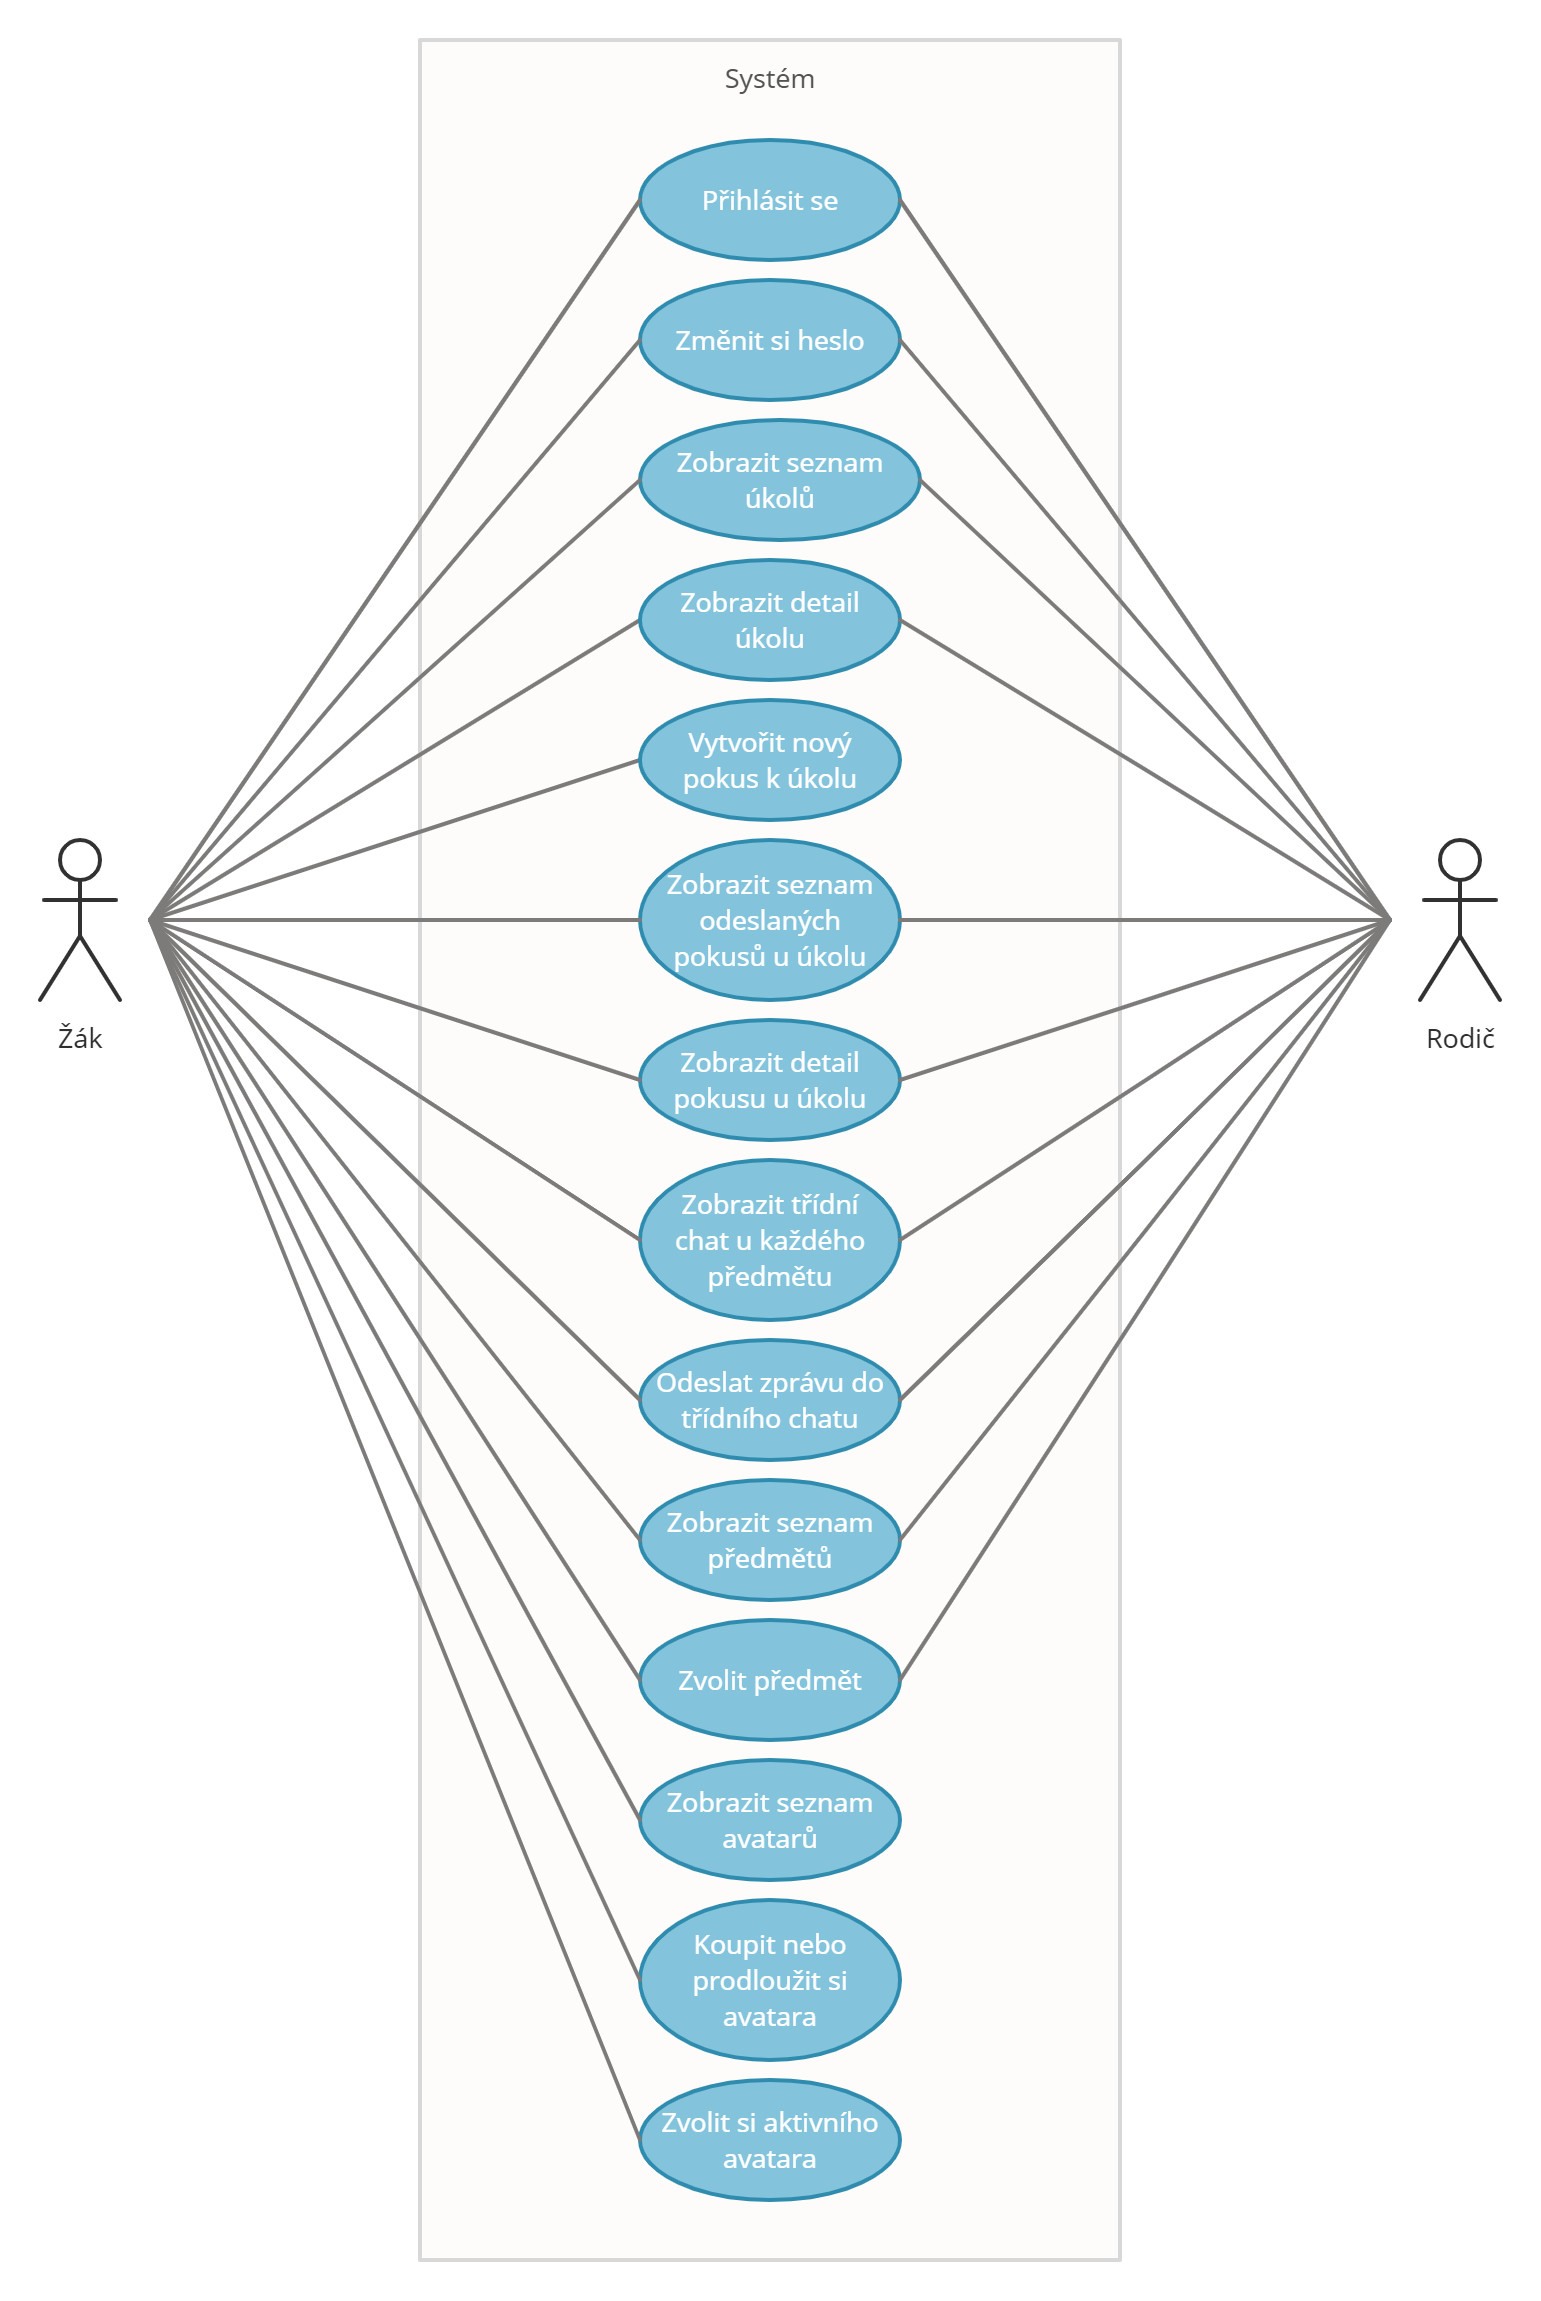
\includegraphics[width=\textwidth]{images/zak_a_rodic}
    \label{img:usecase_zak_a_rodic}
\end{figure}

\begin{figure}
    \caption{Diagram případů užití -- učitel a administrátor}
    \centering
    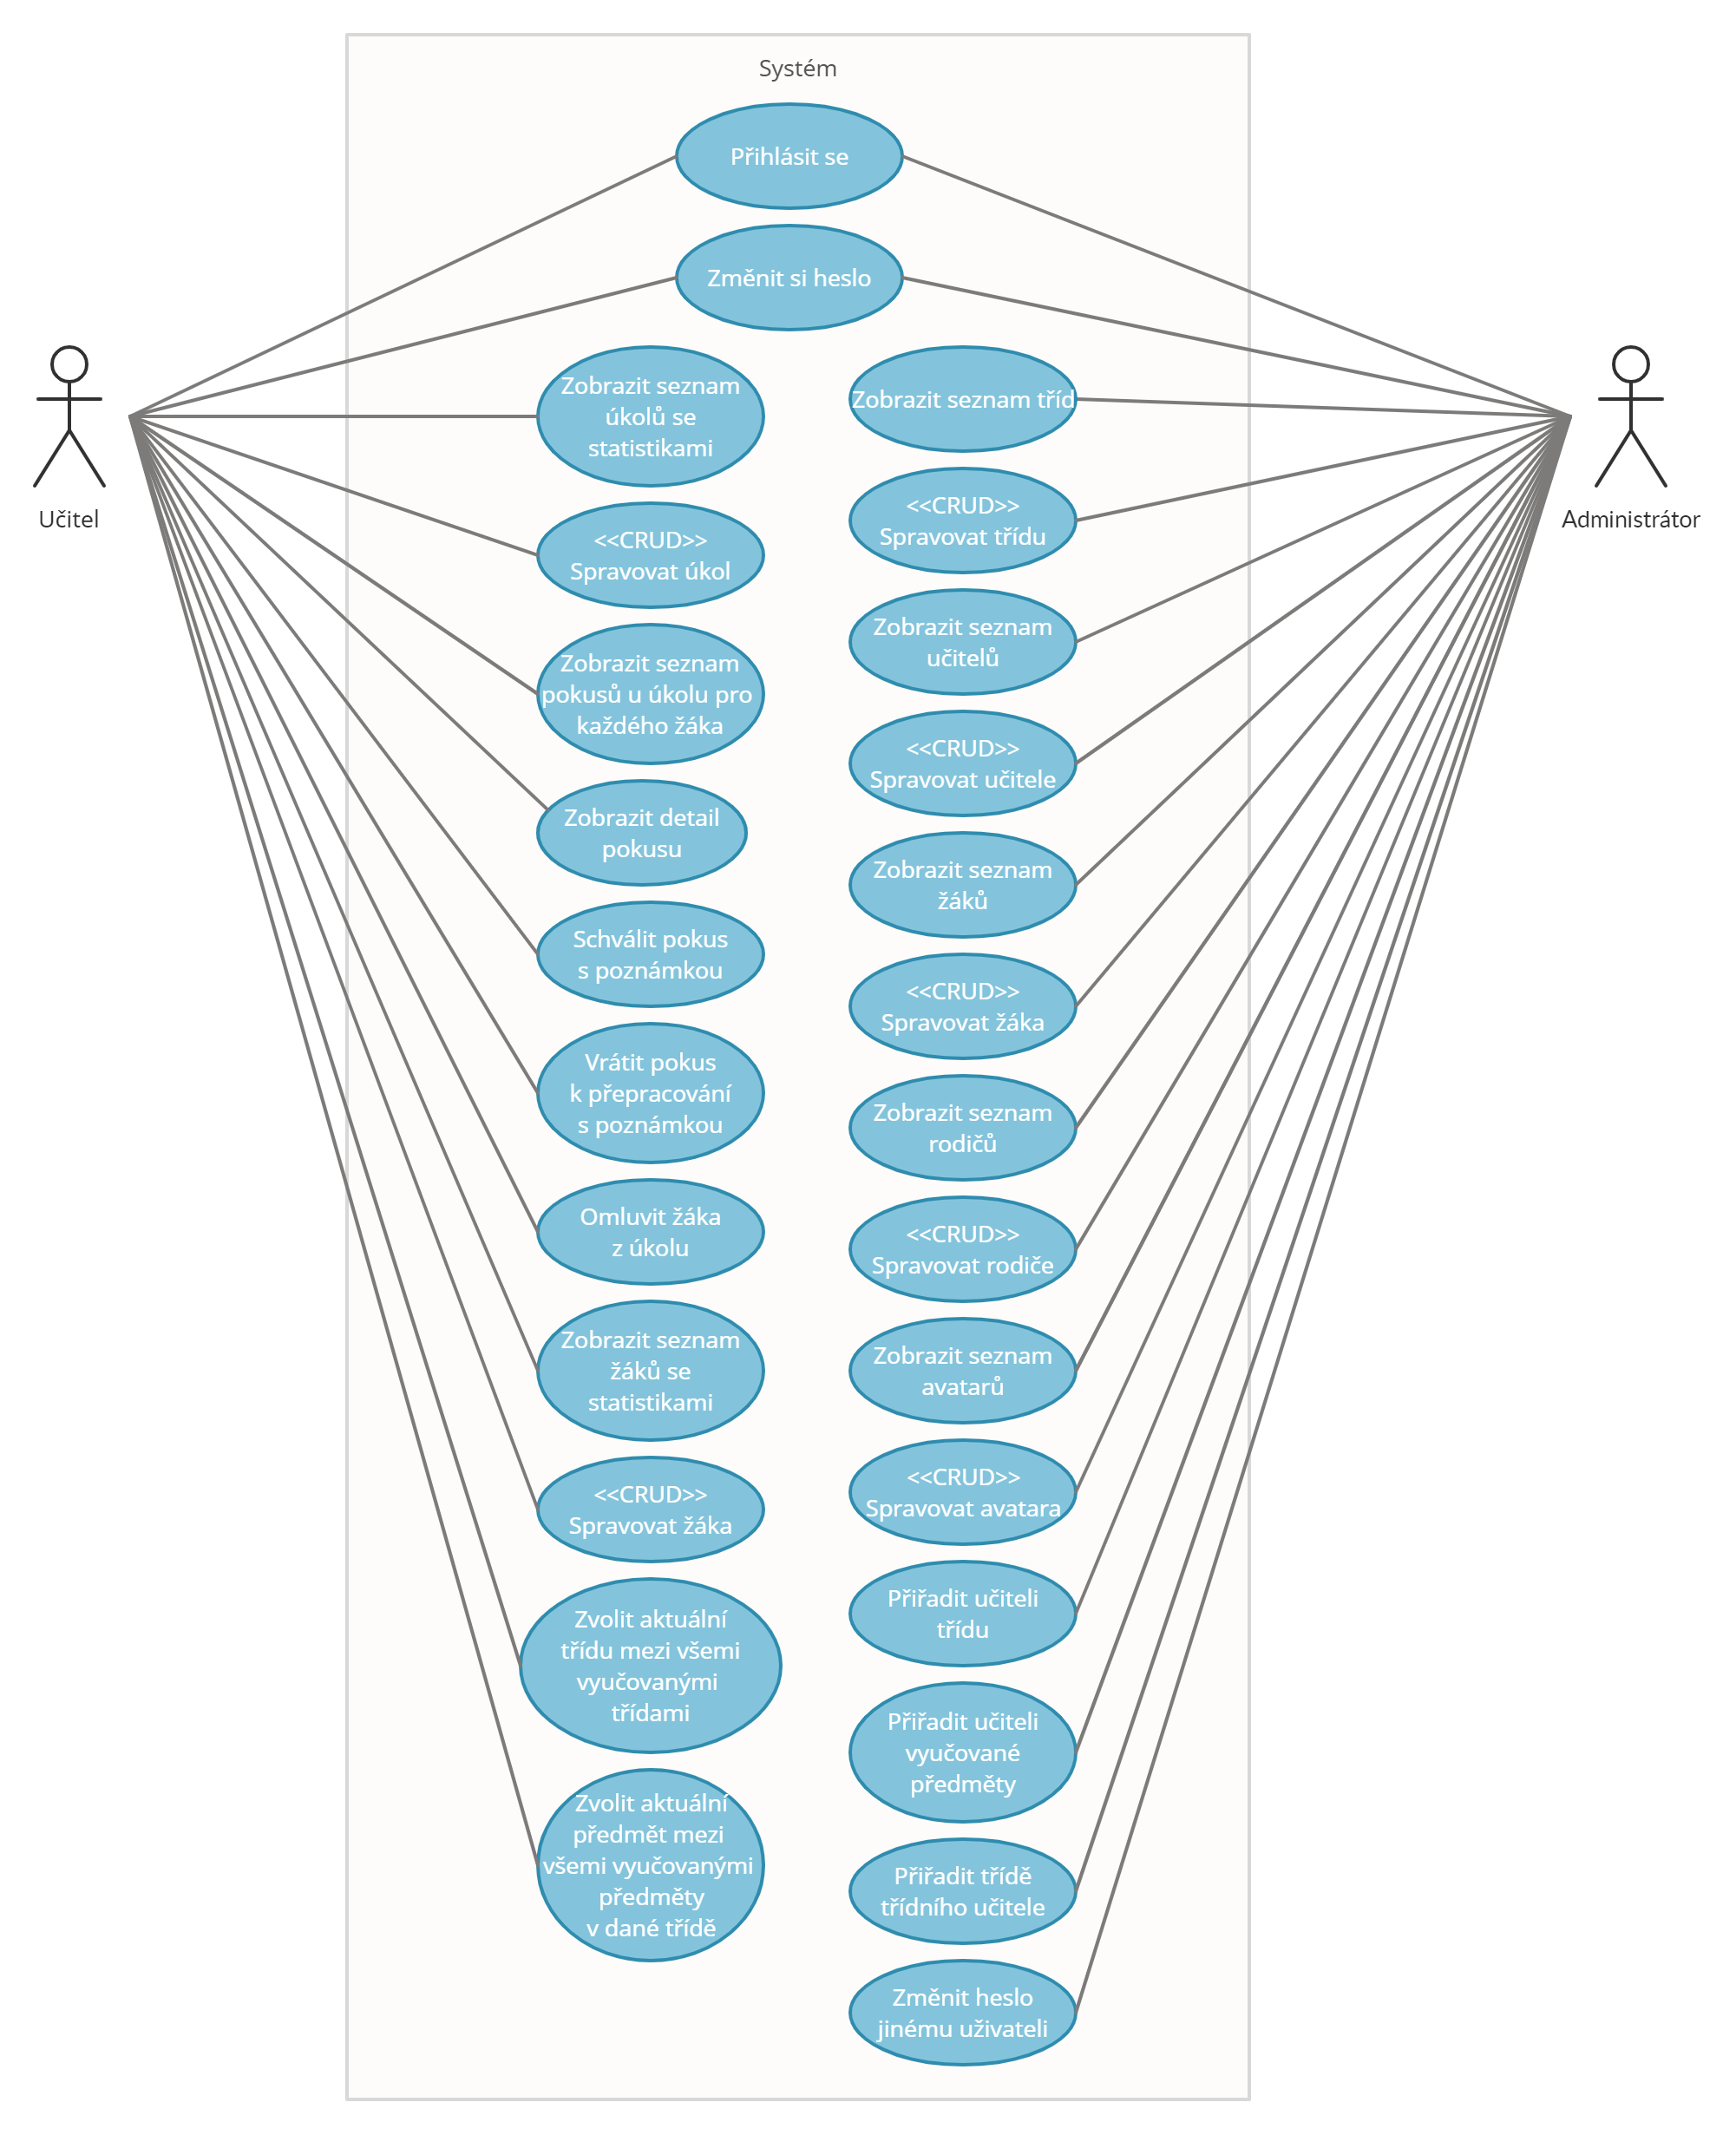
\includegraphics[width=\textwidth]{images/ucitel_a_admin}
    \label{img:usecase_ucitel_a_admin}
\end{figure}











%!TEX ROOT=ctutest.tex

\chapter{Existující řešení}
\label{chap:existujici-reseni}

V následující kapitole rozeberu konkurenční systémy, které se již pokouší požadovanou funkcionalitu implementovat. U každého z nich zmíním nejprve obecné informace k čemu slouží a následně se zaměřím na jejich klady a zápory. Zároveň bych rád zmínil, že u některých systémů nebylo zrovna snadné si je vyzkoušet a provést nějakou analýzu. Důvodem je to, že ne všechny zmiňované systémy jsou zdarma a přístupné široké veřejnosti. Abych uvedl příklad, tak Google Classroom je možné využívat pouze skrz školní účet registrovaný u některé školy, která si tento systém platí. Podobný problém je i pro většinu dalších systémů. Tuto nepříjemnost jsem řešil většinou tak, že jsem vycházel například z různých návodů pro užívání těchto systémů dostupných na internetu.






\section{Microsoft Teams}

V současné době pro nás, jakožto studenty ČVUT, velmi známý a hojně využívaný nástroj. Ukázku uživatelského rozhraní lze vidět na obrázku \ref{img:teams}.

Rozhodně tedy patří k těm populárnějším, a to nejen ve školách, ale zejména i ve firemní sféře. Jedná se totiž o produkt z dílny Microsoftu, díky čemuž nabízí nadstandardní možnosti integrace s dalšími nástroji jako například cloudové úložiště, poznámkové bloky a hlavně umožňuje napřímo editovat dokumenty ve formátu .docx.

Samozřejmě jej lze doplnit i o další pluginy jako například Microsoft Planner pro plánování nejrůznějších úkolů a podobně.

Všechno toto lze samozřejmě považovat za obrovskou výhodu, a to převážně v již zmiňovaných firmách. Nebo obecně tam, kde si lidé s takto komplexním nástrojem poradí. Například tedy i vysoké či některé střední školy.

Tak velké množství funkcí se ovšem může stát nevýhodou v těch oblastech, kde je vyžadována spíše jednoduchost a co nejvyšší uživatelská přívětivost, a to rozhodně základní školy jsou. Takoví uživatelé ocení spíše systém, přesně šitý na míru jejich potřebám. Budou rádi, když nebudou muset nikde nastavovat žádné oprávnění a podobné věci. Nakonec by také mohli mít problém s vícero Microsoft účty, mezi kterými by potřebovali přepínat. Například pracovní a osobní.

\begin{figure}[H]
    \caption{Ukázka uživatelského rozhraní Microsoft Teams, vlastní screenshot}
    \centering
    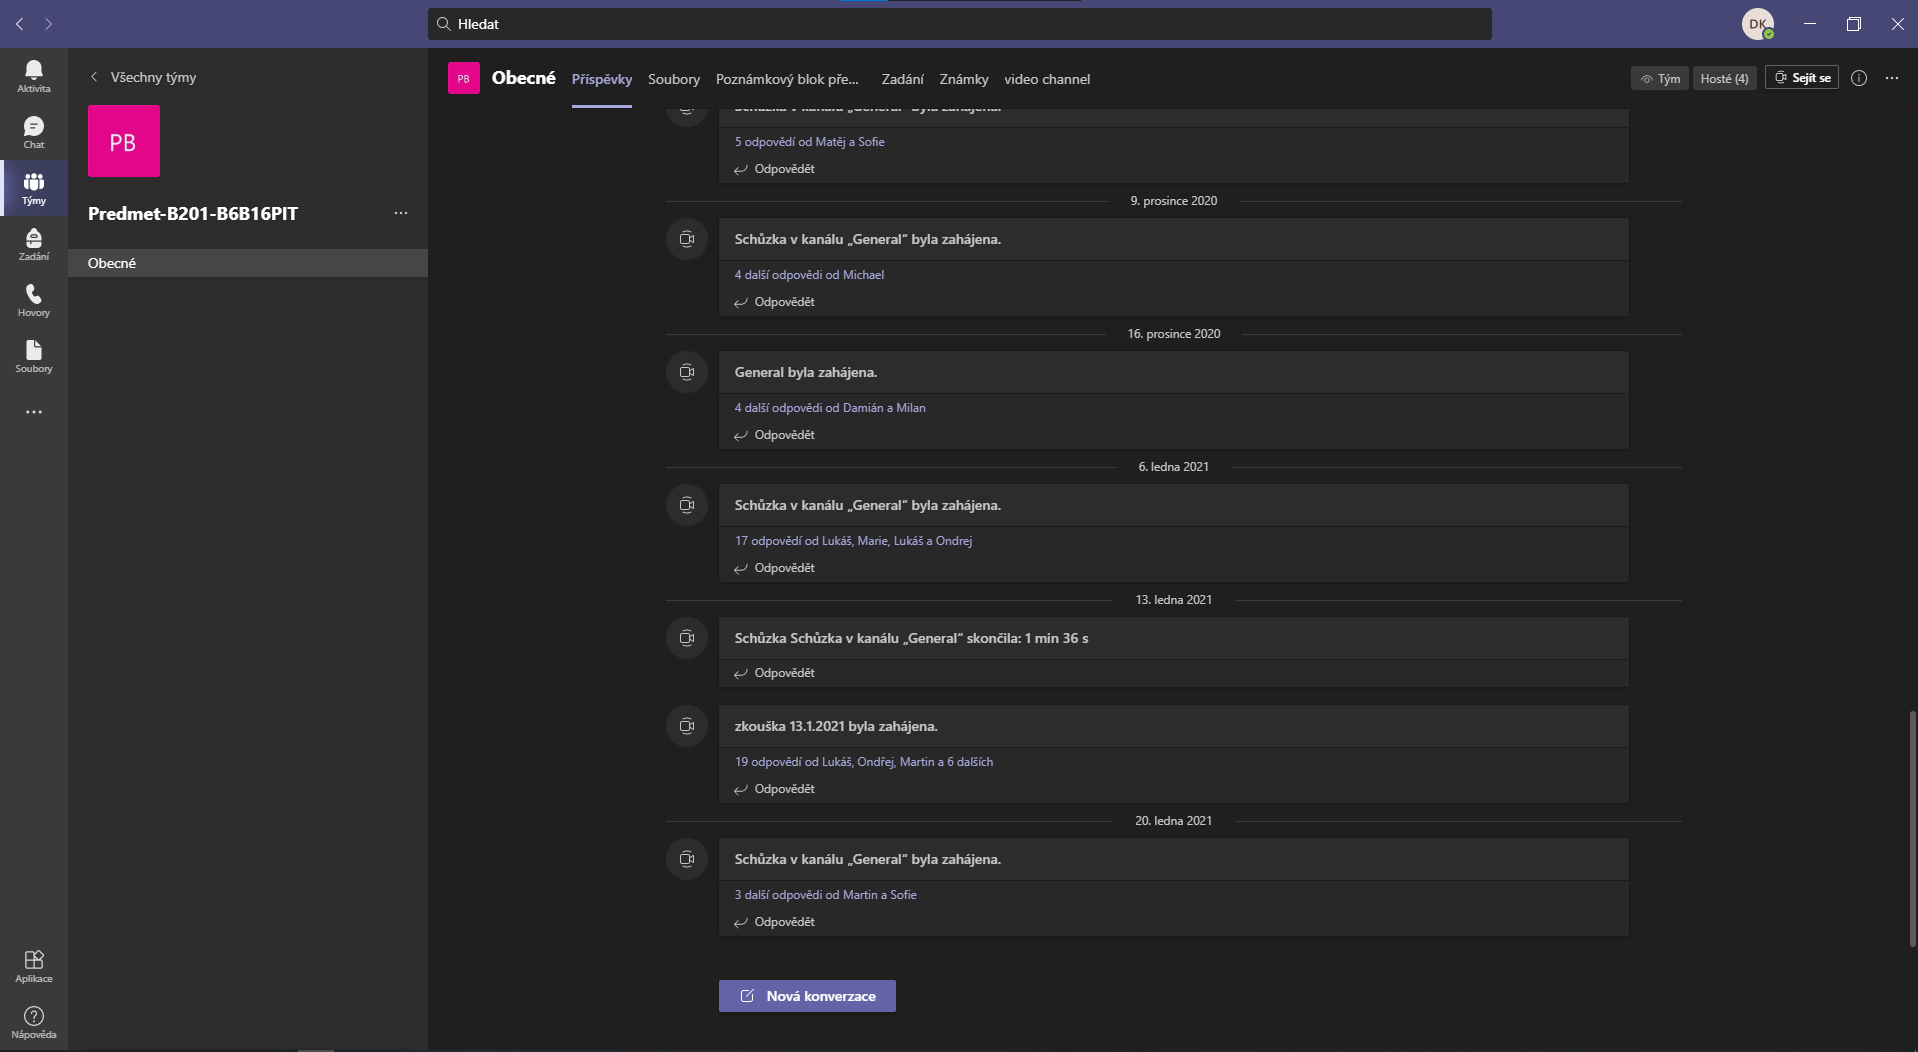
\includegraphics[width=\textwidth]{images/teams}
    \label{img:teams}
\end{figure}

Za výhody lze tedy považovat:
\begin{itemize}
  \item Vysoká možnost integrace s dalšími nástroji
  \begin{itemize}
    \item MS Office
    \item OneNote
    \item OneDrive
    \item a další...
  \end{itemize}
  \item Podpora velké firmy a kvalitní zázemí
  \item Poměrně rozšířený a prozkoušený systém.
  \item Dostupná mobilní aplikace
\end{itemize}

Na druhou stranu, nedostatky jsou například:
\begin{itemize}
  \item Přílišná komplexnost vzhledem k základním školám (nabízí příliš mnoho nepotřebných možností a funkcí)
  \item Naopak postrádá například propracovanější systém pro odevzdávání a kontrolu úkolů
  \item Nedostatečné možnosti nastavení práv
    \begin{itemize}
    \item Skrýt některé kanály v týmu pro určité uživatele
    \item Vymezit pro hosta, co přesně může a nemůže vidět
  \end{itemize}
  \item Nutnost vytvářet si sám strukturu týmů a skupin. Toto často vede k nekonzistentním stavům, kde například každý předmět je trochu jinak uspořádaný a uživatel je poté velmi zmatený.
  \item Při posílání dokumentů je zde potřeba myslet na adresářovou strukturu, aby zůstal obsah přehledný. Toho nemusí být malé děti schopné a i pro dospělé to může být obtěžující.
\end{itemize}


\section{Google Classroom}

O něco více se potřebám škol snaží přiblížit platforma Google Classroom. Ukázku jejího rozhraní lze vidět na obrázku \ref{img:google_classroom}. Nicméně i ta má několik nedostatků.

Abych začal výhodami, tak musím zmínit poměrně čisté a hezké uživatelské rozhraní, které i přes svou jednoduchost nabízí spoustu skvělých funkcí.

Učitel má možnost vytvářet nové kurzy, do kterých může přidávat témata s jednotlivými úkoly nebo může jen psát příspěvky.

Do těchto kurzů se musí žáci přihlašovat sami pomocí kódu. Už to by se dalo považovat za nevýhodu, protože sice se může zdát, že to ušetří práci učiteli, nicméně dovedu si představit, že s tím některý žák bude mít problém a ve finále učitel stejně žádný čas neušetří, protože bude muset žákovi pomoct se do kurzu dostat. V tomto ohledu se mi tedy jeví jako lepší varianta to, že žák dostane již vytvořený účet, který je připojen do všech předmětů ve třídě.

Výhodou může být integrace s dalšími nástroji od společnosti Google. Například Google dokumenty, tabulky, Google disk a podobně. Nicméně i to s sebou nese spoustu problémů, které popisuji v dalším odstavci.

Mezi velké nevýhody patří to, že se uživatel musí přihlašovat svým školním Google účtem. Z toho plyne několik problémů. Jednak jsem se často setkal s uživateli, kteří ani nevědí, že nějaký Google účet mají. Ale mnohem horší je pak přepínání účtů. Téměř každý uživatel má, ať už nevědomky nebo vědomě, svůj osobní Google účet, ale najednou se musí přihlašovat pomocí jiného. Už to může být pro velkou část uživatelů dost zmatečné, a navíc se k tomu pak přidají podobné problémy například při použití Google disku nebo Google dokumentů či fotek. Uživatel je například na svém mobilním telefonu přihlášen pod svým osobním účtem, něco vyfotí, myslí si, že to najde na počítači ve svých Google fotkách, ale pod jiným účtem tyto fotky nenajde.

\begin{figure}[H]
    \caption{Ukázka uživatelského rozhraní Google Classroom, převzato z \cite{google_classroom}}
    \centering
    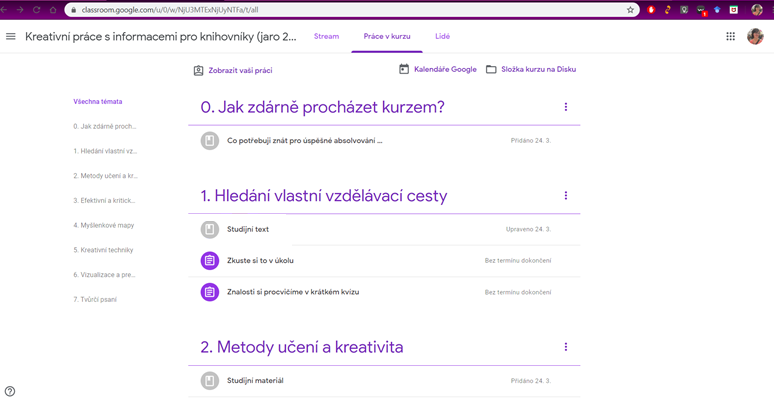
\includegraphics[width=\textwidth]{images/google_classroom}
    \label{img:google_classroom}
\end{figure}

Výhody jsou tedy podobné jako u MS Teams:
\begin{itemize}
  \item Integrace s dalšími Google nástroji
  \begin{itemize}
    \item Google fotky
    \item Google dokumenty, tabulky
    \item Google disk
    \item a další...
  \end{itemize}
  \item Podpora velké společnosti a kvalitní zázemí
  \item Poměrně rozšířený a zaběhlý systém
  \item Čisté a moderní uživatelské rozhraní
  \item Dostupná mobilní aplikace
\end{itemize}

Ovšem i zde existují nedostatky:
\begin{itemize}
  \item Přepínání Google účtů (osobní, školní)
  \item Žáci se musí dostat do kurzů sami
  \item Odevzdávání řešení
  \begin{itemize}
    \item Žák může buď psát přímo do zadání, pak si ho ale může, byť jen omylem, změnit.
    \item Nebo může mít práva zadání pouze zobrazit. Pak je pro něj ale situace složitější v tom, že musí vytvořit nový dokument a poradit si s formou sám. Buď zadání zkopíruje a dopisuje do něj nebo se na otázky nějak odkazuje např. čísly.
  \end{itemize}
  \item Nepropracované multiple choice úkoly v porovnání např. s Moodle (chybí kupříkladu poměrné bodové hodnocení za částečné řešení)
\end{itemize}

\section{Bakaláři}

Nyní už se dostávám k nástroji, který se skutečně snaží pokrýt potřeby škol. Uživatelům poskytuje nepřeberné množství funkcí včetně například plánovaných akcí školy, knihovny, suplování a další. Právě tyto, z mého pohledu, trochu nadbytečné funkce činí ovšem tento systém hovorově řečeno "přeplácaný" jak lze vidět na ukázce \ref{img:bakalari}.

Samozřejmě netvrdím, že je to úplně špatně. Tento nástroj je přeci jen stavěn spíše pro kompletní pokrytí všech požadavků škol, což splňuje dobře. Nicméně předmětem mé práce je přijít s řešením, které bude velmi jednoduché a intuitivní pro všechny druhy uživatelů a to jde trochu proti sobě s pokrytím všech myslitelných požadavků.

S předchozím bodem také souvisí historický vývoj této platformy, která byla původně koncipována jako desktopová aplikace. V současné době je ovšem zájem spíše o webové rozhraní, a tak vzniká nekonzistence mezi těmito dvěma prostředími. Jednak vypadají rozdílně, a navíc poskytují rozdílné funkcionality, což může být velice matoucí.

Také je nutno podotknout, že systém Bakaláři je v některých ohledech vcelku "nedotažený". Například bych rád zmínil proces zadávání a schvalování úkolů. Ze sesbíraných referencí vím, že učitelé často zapomenou označit úkol za dokončený, když ho odevzdají všichni studenti. Pak se stává to, že ho i nadále všichni studenti vidí ve svém seznamu úkolů a časem se z tohoto seznamu stane nepořádek. Lepší by bylo, kdyby se žákovi úkol po schválení přestal zobrazovat v seznamu a případně se přesunul do nějakého méně nápadného seznamu odeslaných či hotových úkolů. Učitel by pak viděl úkol také jen do té doby než ho dořeší všichni studenti a následně by se automaticky označil jako dokončený a také by se přesunul do jiného seznamu.

\begin{figure}[H]
    \caption{Ukázka uživatelského rozhraní Bakaláři, převzato z \cite{bakalari}}
    \centering
    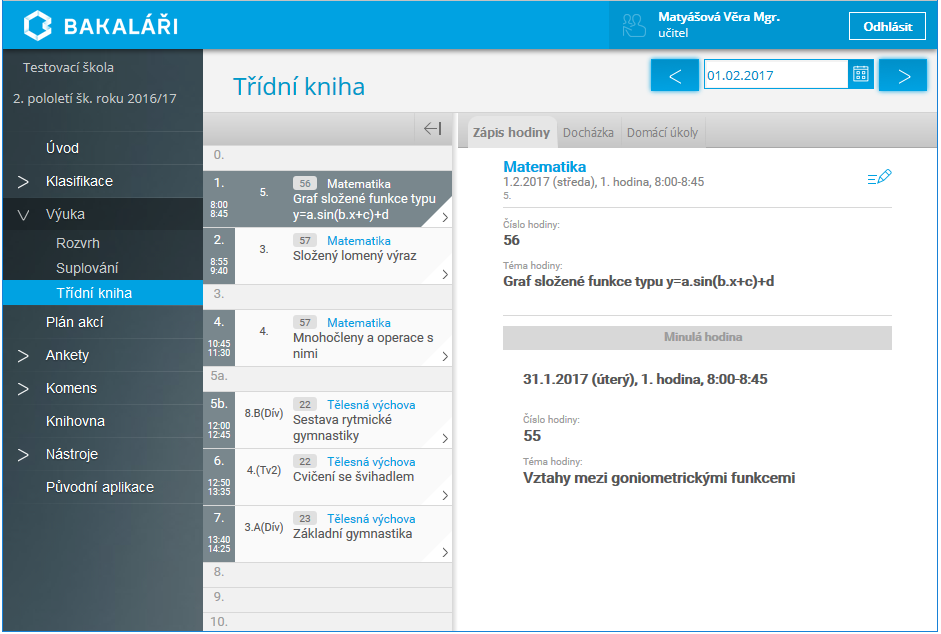
\includegraphics[width=\textwidth]{images/bakalari}
    \label{img:bakalari}
\end{figure}

Výhody:
\begin{itemize}
  \item Snaha o kompletní pokrytí všech požadavků škol
  \item Dostupné výukové materiály pro práci se systémem
  \item Dostupná mobilní aplikace
  \item Vhodné spíše pro úplnou digitalizaci školy
\end{itemize}

Nedostatky:
\begin{itemize}
  \item Náročnější k naučení se všech možných funkcí
  \item Příliš komplexní (vzhledem k požadavku na co největší jednoduchost nabízí tento systém příliš nepotřebných funkcí, například akce školy, knihovny, atd.)
  \item V některých částech "nedotažené" (např. splnění úkolu)
  \item Různý vzhled a funkce na různých platformách (zejména desktopová a webová aplikace)
  \item Často padá či nefunguje.
  \begin{itemize}
      \item To může být způsobeno historicky použitím různých programovacích jazyků a technologií
  \end{itemize}
\end{itemize}


\section{Škola OnLine}

Tato platforma je poměrně dost podobná zmiňovaným Bakalářům. Možná i to je důvod proč se tyto platformy v roce 2019 spojily. Také se snaží pokrýt většinu požadavků škol a i když není zatím tolik komplexní, také je poměrně těžkopádná. Ukázku uživatelského rozhraní lze vidět na obrázku \ref{img:skolaonline}

\begin{figure}[H]
    \caption{Ukázka uživatelského rozhraní Škola OnLine, převzato z \cite{skolaonline}}
    \centering
    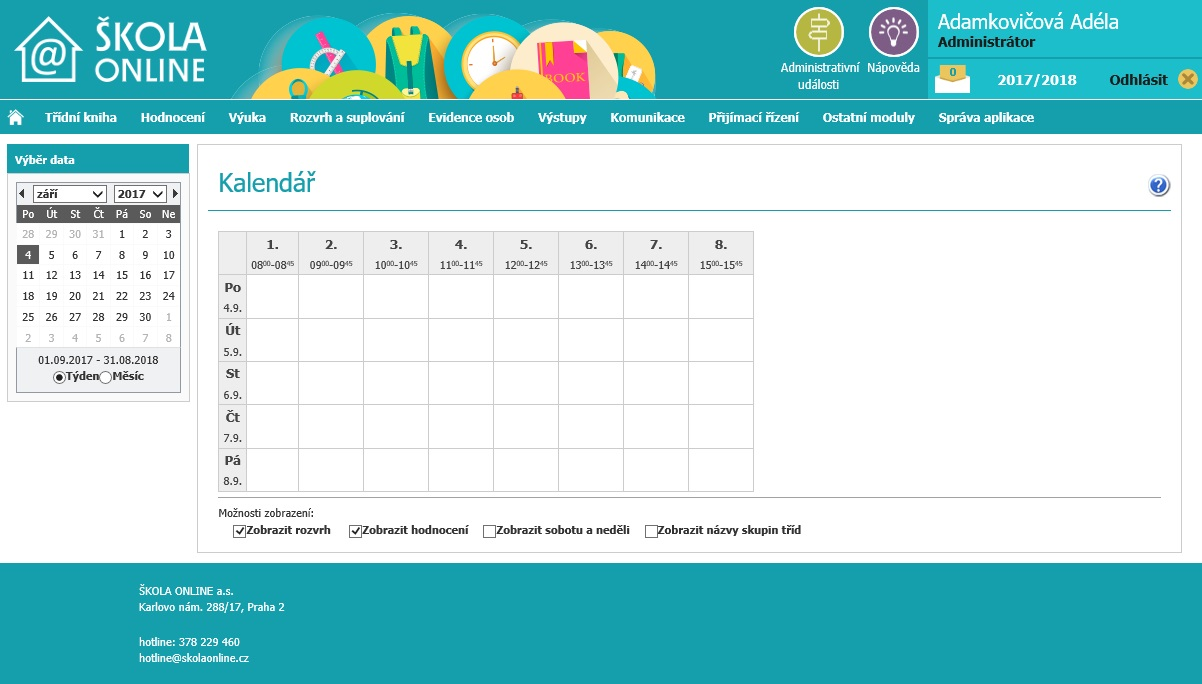
\includegraphics[width=\textwidth]{images/skola_online}
    \label{img:skolaonline}
\end{figure}
\newpage
Výhody:
\begin{itemize}
  \item Snaha o kompletní pokrytí všech požadavků škol
  \item Dostupné výukové materiály pro práci se systémem
  \item Dostupná mobilní aplikace
  \item Vhodné spíše pro úplnou digitalizaci školy
\end{itemize}

Nedostatky:
\begin{itemize}
  \item Příliš komplexní (podobně jako Bakaláři, tak i Škola OnLine nabízí vzhledem k požadavku na co nejvyšší jednoduchost příliš nepotřebných funkcí, například knihovna, školní akce)
  \item Neintuitivní uživatelské rozhraní (Pomohly by například jen drobnosti jako, aby názvy úkolů a podobné nápisy fungovaly jako odkazy)
\end{itemize}


\section{Škola v pyžamu}

Poměrně hezkým projektem je Škola v pyžamu, jehož uživatelské rozhraní lze vidět na obrázku \ref{img:skola_v_pyzamu}. Zde se autoři snaží právě o jednoduchost, kterou rodiče a malé děti ocení nejvíce. Nicméně zde na druhou stranu zase několik věcí chybí. Například učitel si nemůže psát k žákům různé poznámky či nevidí přehledné shrnutí všech úkolů. Vidí pouze úkoly pod sebou a u každého z nich seznam žáků se stavem vypracování. Také by bylo vhodnější rozdělení na jednotlivé předměty a snazší přepínání tříd pro učitele.

\begin{figure}[H]
    \caption{Ukázka uživatelského rozhraní Škola v pyžamu, převzato z \cite{skola_v_pyzamu}}
    \centering
    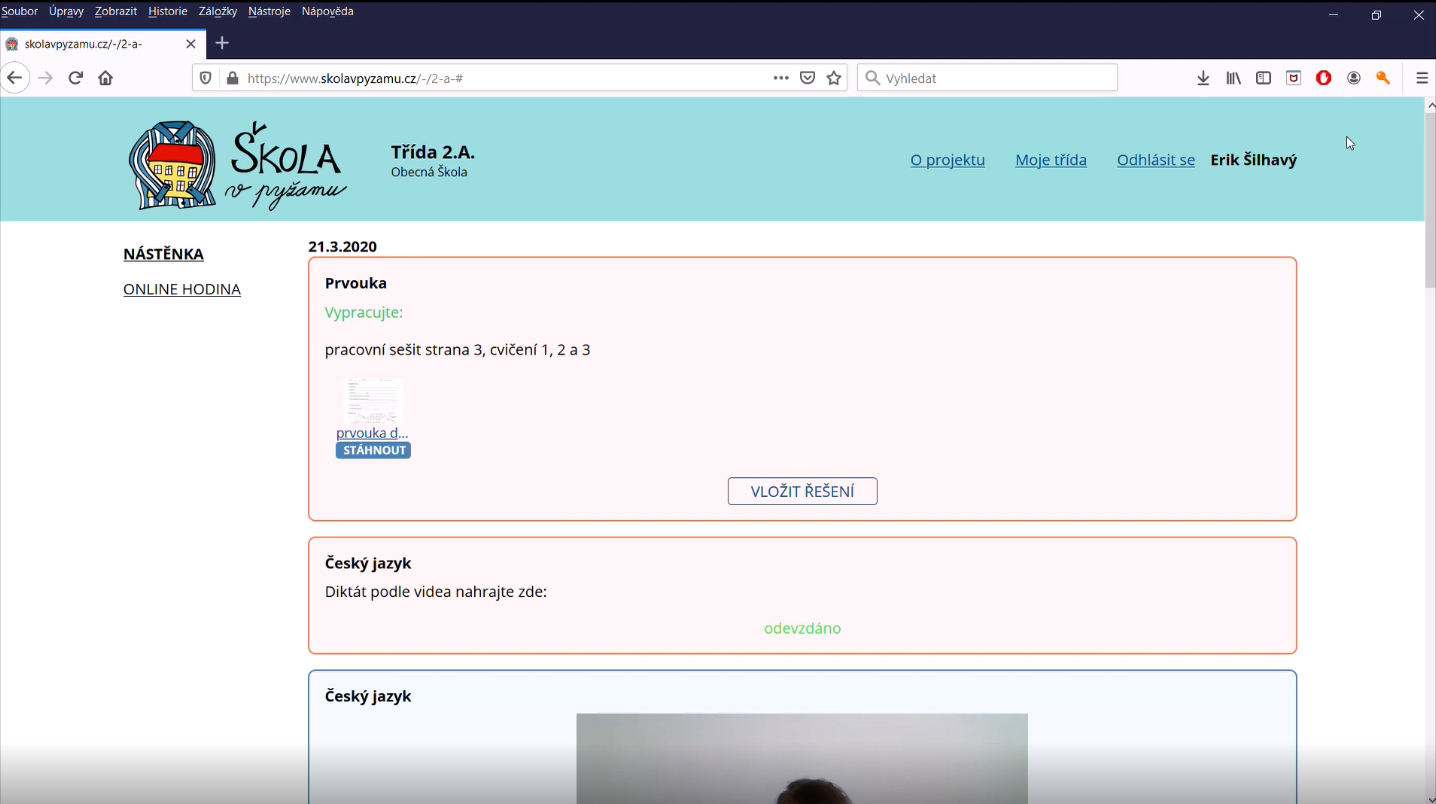
\includegraphics[width=\textwidth]{images/skola_v_pyzamu}
    \label{img:skola_v_pyzamu}
\end{figure}

Výhody:
\begin{itemize}
  \item Velmi jednoduché prostředí (dáno ovšem absencí některých funkcí)
  \item Zdarma
\end{itemize}

Nedostatky:
\begin{itemize}
  \item Chybí mobilní aplikace
  \item Chybí lepší rozdělení jednotlivých předmětů
  \item Složité přepínání mezi třídami
\end{itemize}


\section{Moodle}

Tento systém je znám spíše na vysokých školách. Jedná se o poměrně komplexní nástroj, který umožňuje i tvorbu testů různých druhů, systém známkování, multijazyčnost a další. Nicméně, jak již vyplývá z faktu, kde se využívá, není jeho využití pro základní školy příliš vhodné. Přeci jen není tolik intuitivní, jak by bylo potřeba. Navíc je vhodné pro jeho konfiguraci mít k dispozici IT odborníka, kterých nebývá na základních školách dostatek. Ukázku jeho uživatelského rozhraní lze vidět na obrázku \ref{img:moodle}.

\begin{figure}[H]
    \caption{Ukázka uživatelského rozhraní Moodle, vlastní screenshot}
    \centering
    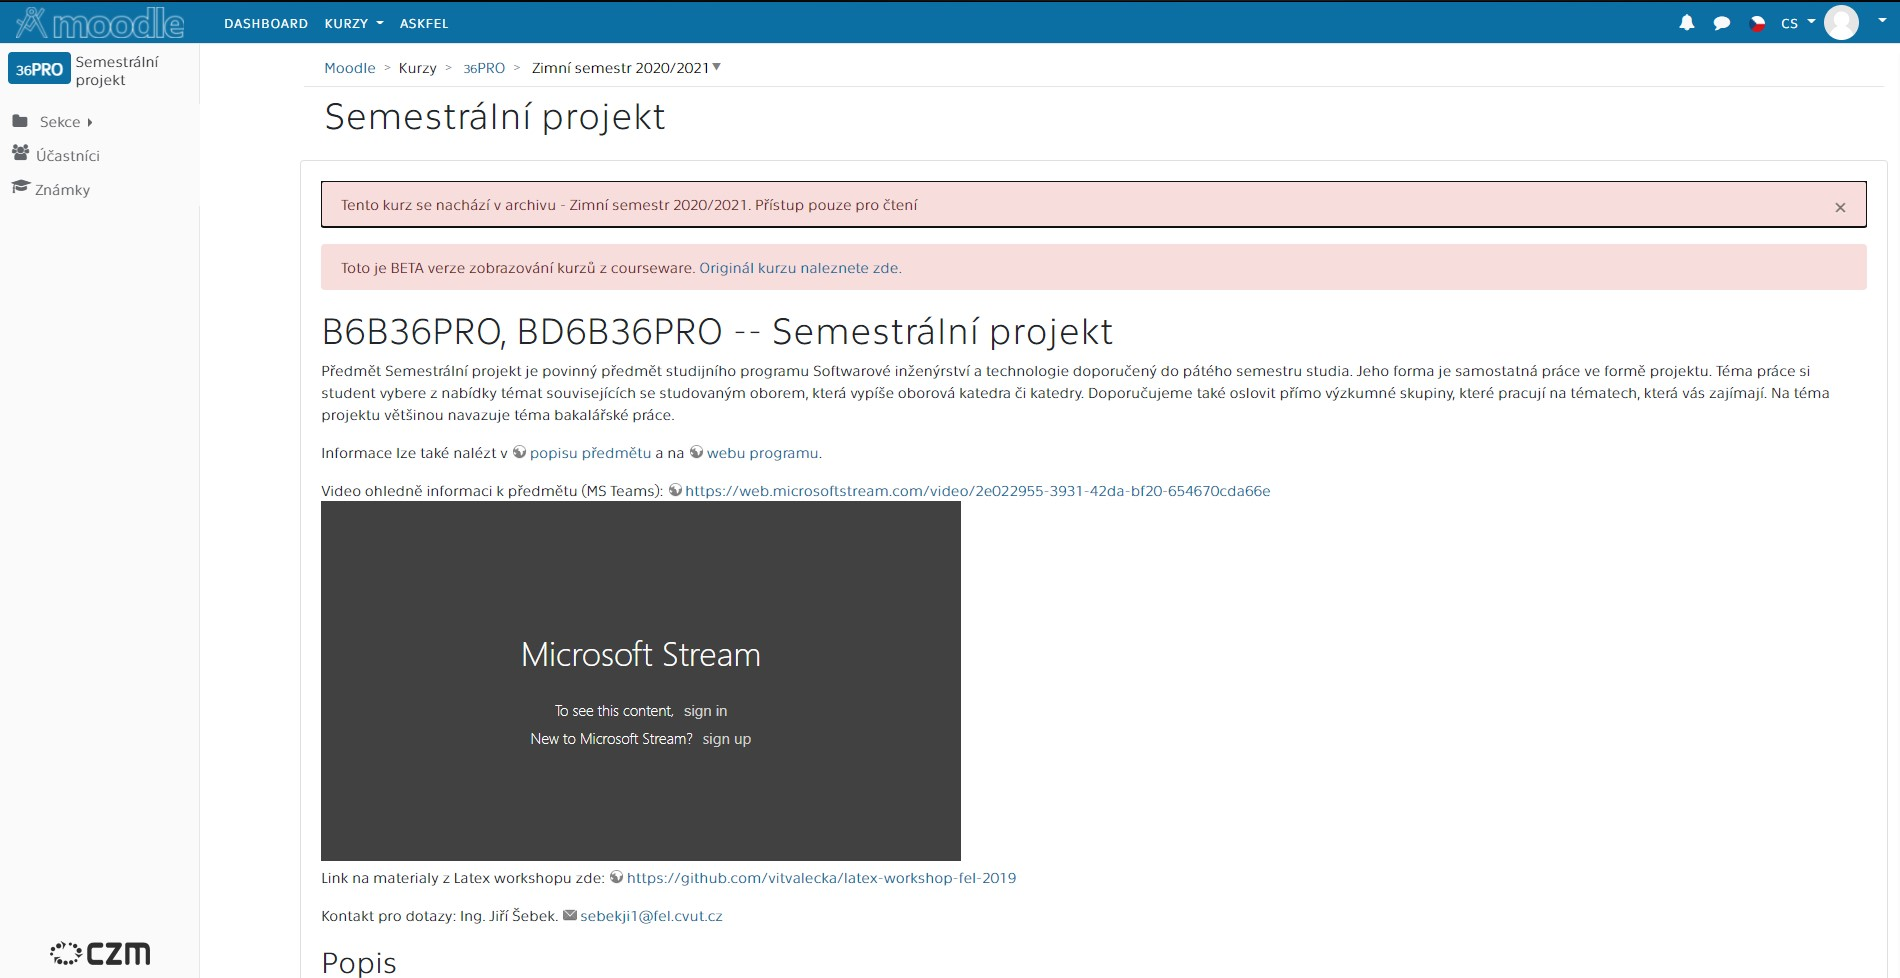
\includegraphics[width=\textwidth]{images/moodle}
    \label{img:moodle}
\end{figure}

Výhody:
\begin{itemize}
  \item Poměrně dobré možnosti tvorby online testů
  \begin{itemize}
    \item Průběžné odesílání řešení pomocí AJAX
    \item Možnost nastavit poměrné bodové hodnocení částečně správných řešení
  \end{itemize}
  \item Různé role uživatelů
\end{itemize}

Nedostatky:
\begin{itemize}
  \item Nepříliš intuitivní
  \begin{itemize}
      \item Například na úvodní stránce by bylo dobré u každého předmětu vidět přehled toho, co je potřeba udělat.
  \end{itemize}
  \item Má problémy na mobilních zařízeních, kde někdy dokonce není vidět část obsahu.
  \item Složitější konfigurace
\end{itemize}

\section{Online cvičení}

Tento web je zaměřen trochu jinak. Je vhodný spíše pro procvičování různých typů cvičení. Žák zde nalezne spoustu dostupných úkolů, ale tím výhody v podstatě končí. Celkově systém není příliš "dotažený". Například přidávání do skupin probíhá zbytečně složitým způsobem, kdy se žák musí sám registrovat, vyhledat podle kódu skupinu, žádat admina o přidání a pak doufat, že ho admin přidá. Mnohem jednodušší se mi jeví řešení, kdy toto vše vyřídí za žáky sám učitel. Ukázku tohoto webu lze vidět na obrázku \ref{img:onlinecviceni}.


\begin{figure}[H]
    \caption{Ukázka uživatelského rozhraní Online cvičení \cite{onlinecviceni}, vlastní screenshot}
    \centering
    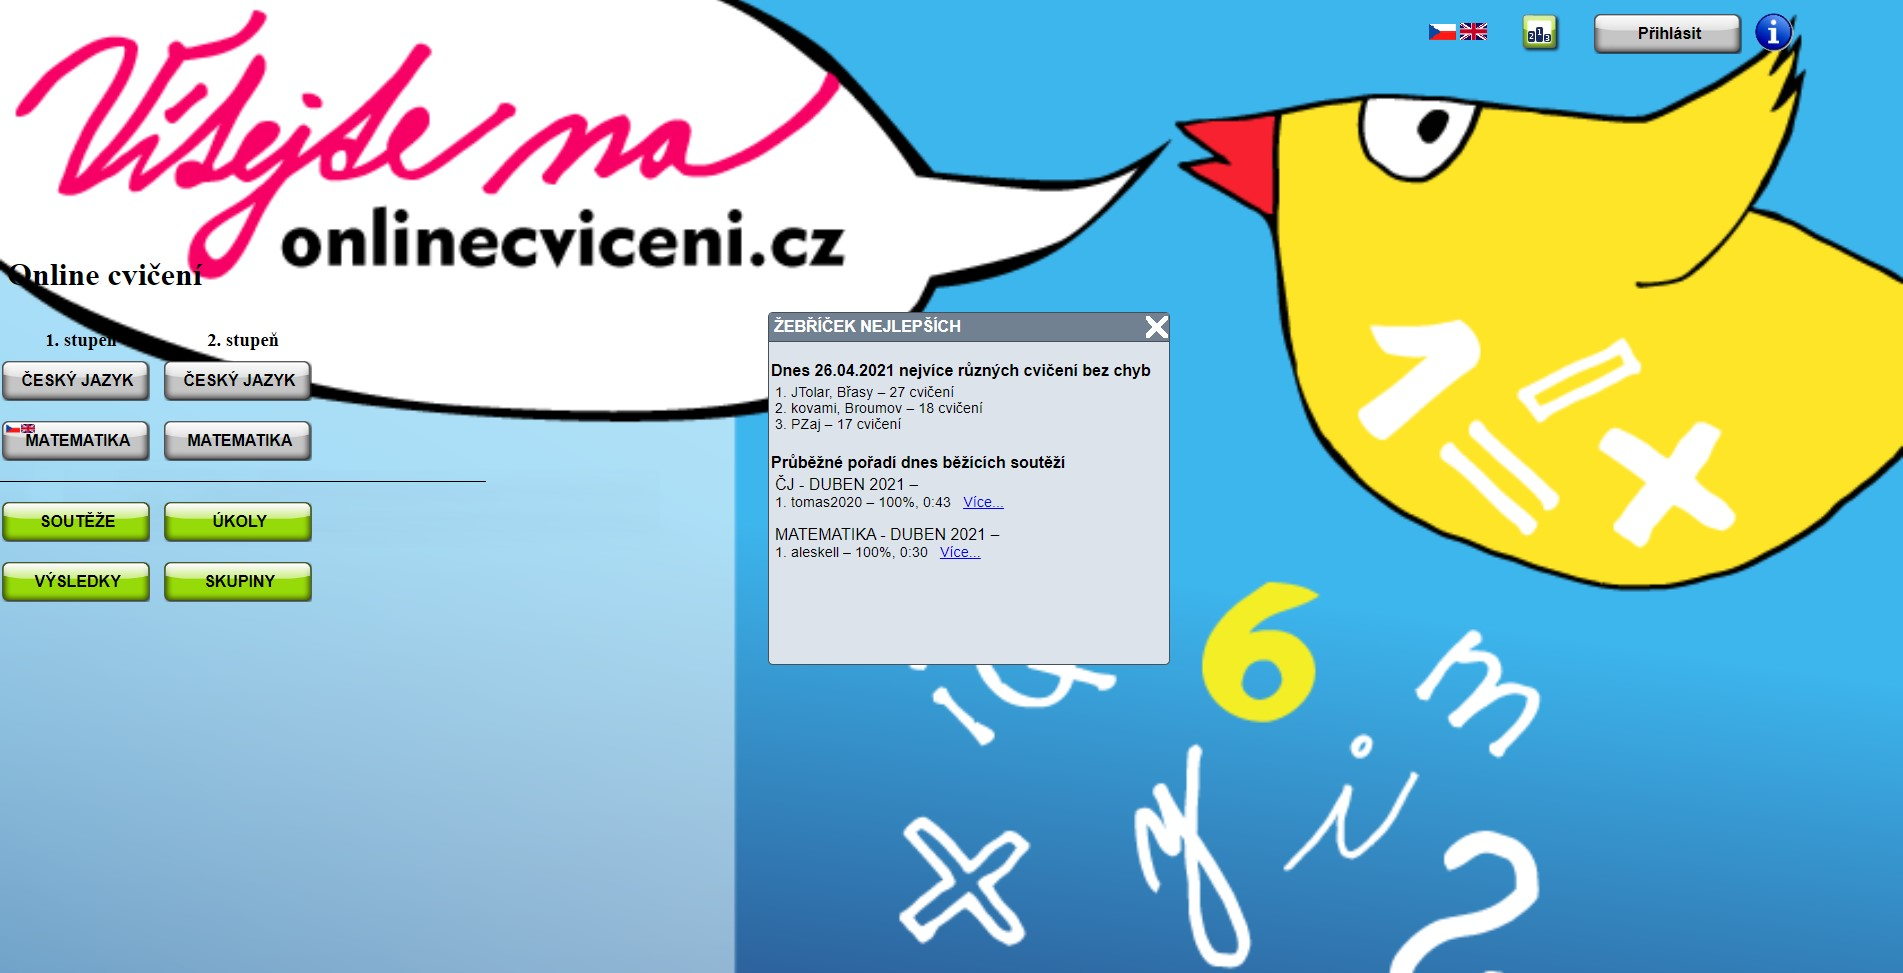
\includegraphics[width=\textwidth]{images/onlinecviceni}
    \label{img:onlinecviceni}
\end{figure}

Výhody:
\begin{itemize}
    \item Velké množství obsahu (různá cvičení)
\end{itemize}

Nedostatky:
\begin{itemize}
    \item Nedotažené (zbytečně složité a nepřehledné vzhledem k tak malému počtu funkcí)
    \item V dnešní době odrazující uživatelské rozhraní
\end{itemize}

\section{Umíme to}

Podobným směrem jako předchozí systém se vydává i Umíme to. Také je zde k dispozici ještě větší škála různých úkolů z různých předmětů. Tento nástroj je ovšem mnohem lépe propracovaný. Nabízí poměrně hezké a čisté uživatelské rozhraní (vizte obrázek \ref{img:umimeto}) a působí uceleným dojmem.

Na druhou stranu i zde vidím několik nedostatků. Stejně jako u předchozího, je zde problém s registrací žáků. Ti se musí registrovat a připojit do třídy opět sami. Může to znít jako maličkost, ale umím si představit, že u dětí na prvním stupni základních škol to nemusí být pro všechny rodiče jednoduché a může to v nich hned od začátku vyvolat ze systému nepříjemný pocit. Pak ani nemusí mít snahu a chuť pochopit samotné funkce, které jsou jim po přihlášení k dispozici.

Také by bylo vhodné učitelům nabídnout více statistik a například psát si ke studentům různé poznámky. Vhod by přišel také třídní chat.


\begin{figure}[H]
    \caption{Ukázka uživatelského rozhraní Umíme to \cite{umimeto}, vlastní screenshot}
    \centering
    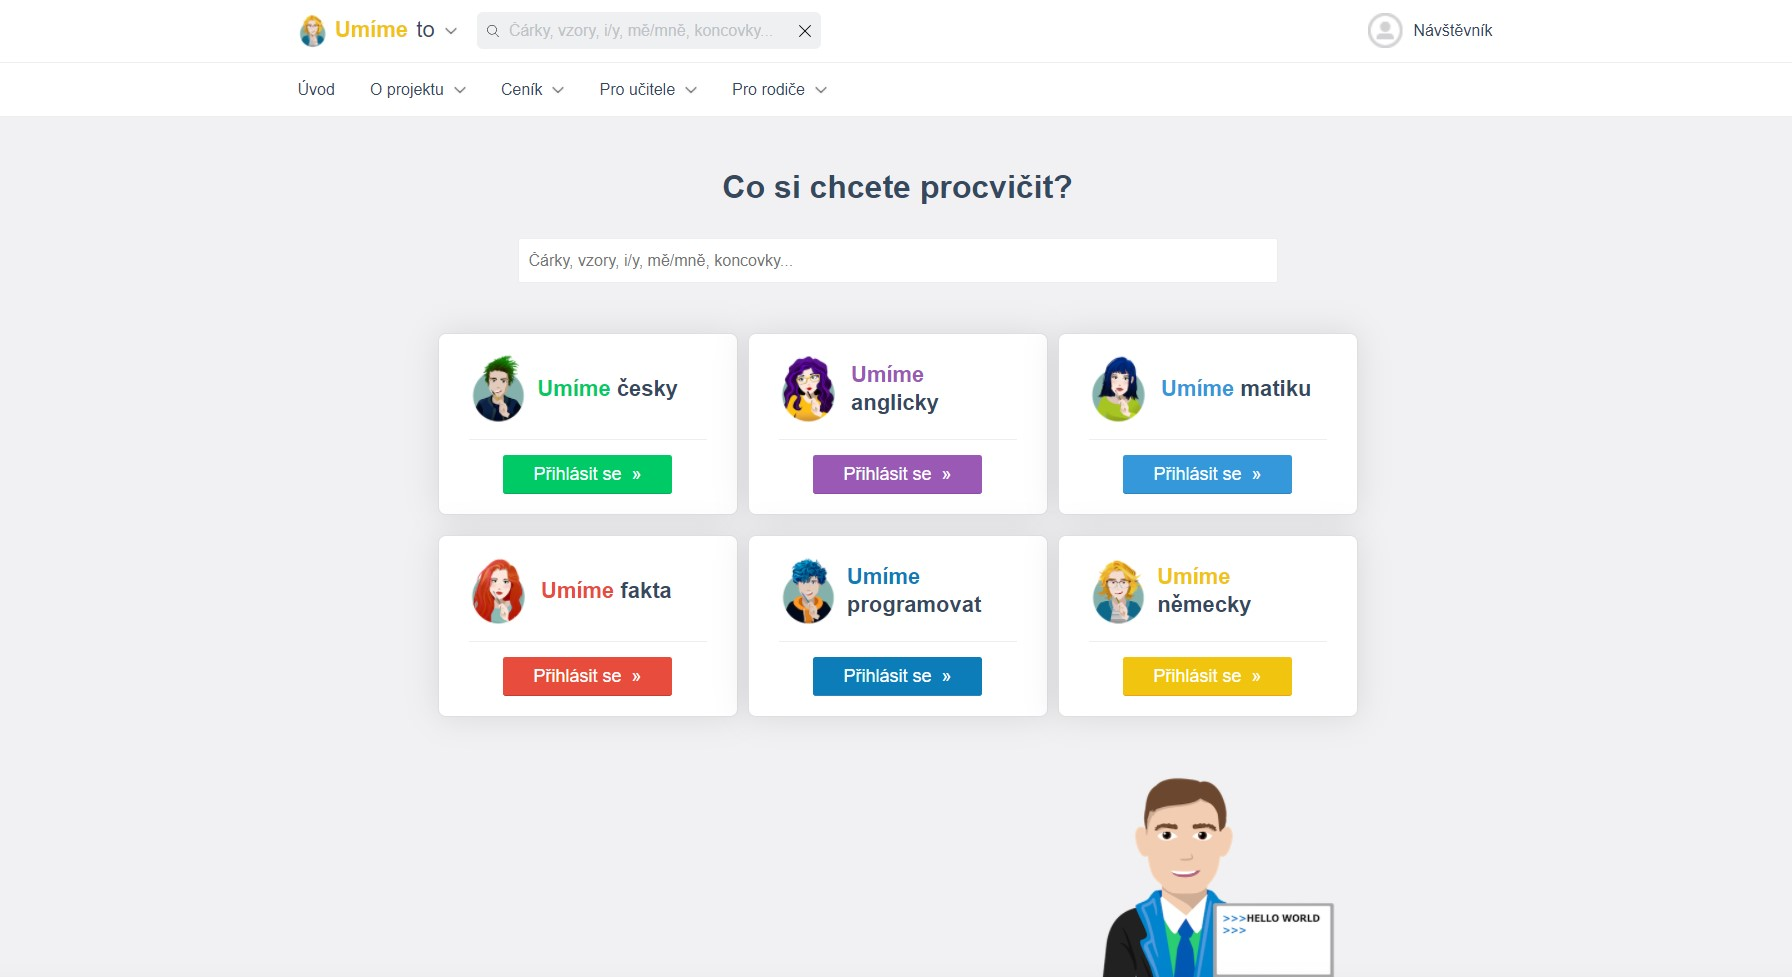
\includegraphics[width=\textwidth]{images/umimeto}
    \label{img:umimeto}
\end{figure}

Výhody:
\begin{itemize}
  \item Hezké a čisté uživatelské rozhraní.
  \item Velká spousta předpřipravených úkolů různých typů
\end{itemize}

Nedostatky:
\begin{itemize}
  \item Omezení jen na předpřipravené úlohy
  \item Málo statistik
  \item Registraci a připojení ke třídě si musí řešit žáci sami
  \item Chybějící chat
\end{itemize}


%\subsection{Classkick - TODO}

\section{Shrnutí}

Z předchozích implementací vychází několik poznatků, které bych zde rád shrnul.

V první řadě většina z nich je příliš složitá pro žáky prvního stupně. Svou implementaci bych tedy měl směřovat hlavně k tomu, aby byla jednoduchá, intuitivní a přehledná.

S tím souvisí další častý problém s registracemi. Bude mnohem jednodušší, když si žáky přidá do třídy rovnou učitel a žáci se pak jen přihlásí uživatelským jménem, které jim je sděleno a zvolí si pouze své heslo.

To samé by mohlo platit i pro samotné učitele a třídy. Ty bude registrovat a vytvářet administrátor a rovnou je k sobě přiřadí. Učitel se tedy jen přihlásí a zvolí si pouze své heslo stejně jako žák. Tím nemusí nic dalšího řešit a může jít rovnou vytvořit účty žákům.

Dále bude potřeba propracovat zadávání a odevzdávání úkolů. Mělo by platit, že zadání může měnit pouze učitel a žák k němu posílá pouze své řešení. To může následně učitel vrátit k přepracování s komentářem, ovšem nesmí upravovat žákovo řešení, aby ho například omylem nesmazal.

Všichni uživatelé musí jasně vidět přehled toho, co musí ještě udělat. Pokud tedy například žák odešle řešení úkolu, tak by se měl tento úkol rovnou přesunout do méně důležité sekce, aby se nepletl s aktuálními povinnostmi.

Snadné by také mělo být přepínání mezi předměty (v případě učitele i mezi třídami).

Vhodnou funkcí je i třídní chat. Ideálně pro každý předmět zvlášť.



\part{Implementace}
\label{part:implementace}





\chapter{Architektura}
\label{chap:architektura}
Nedílnou částí návrhu implementace je architektura samotného řešení, které se věnuje tato kapitola.

\section{Použité technologie}
V této sekci bych rád představil technologie, které jsem se rozhodl použít. U~každé z nich uvedu stručný popis a důvody, proč má v tomto projektu své místo.




\subsection{Jakarta EE}

Jakarta EE je souhrn specifikací, který umožňuje světové komunitě vývojářů vyvíjet jednotlivé navzájem kompatibilní implementace \cite{jakarta}. Ve finále se tedy jedná o velkou platformu ulehčující vývoj enterprise aplikací. Celá tato platforma nabízí nepřeberné množství nástrojů, frameworků a knihoven, které poskytují velmi ucelené prostředí pro vývoj od základu dobře navržených systémů.
%\newpage

\textit{
Obecně se všechny Jakarta EE specifikace skládají z: 
\begin{itemize}
    \item API a dokument specifikace -- definuje a popisuje samotnou specifikaci
    \item TCK (Technology Compatibility Kit) -- slouží k testování jednotlivých implementací založených na výše zmíněných API a specifikačním dokumentu
    \item Kompatibilní implementace -- ty implementace, které úspěšně splnily testy TCK \emph{\cite{jakarta}}
\end{itemize}
}

Velmi pěkný přehled nabízí obrázek \ref{img:jakartaee}. Ukazuje architekturu vícevrstvé webové aplikace na platformě Jakarta EE. Je na něm vidět, jak je vše promyšleně rozdělené, které vrstvy s čím komunikují a v podstatě přesně popisuje principy, kterých jsem se držel při implementaci. Často se tedy na tento diagram budu dále odkazovat z následujících dílčích podkapitol, kde popisuji jednotlivé technologie zapadající do tohoto ekosystému.

\begin{figure}[H]
    \caption{Jakarta EE 8 -- Diagram architektury, převzato z \cite{jakarta:tutorial_diagram}}
    \centering
    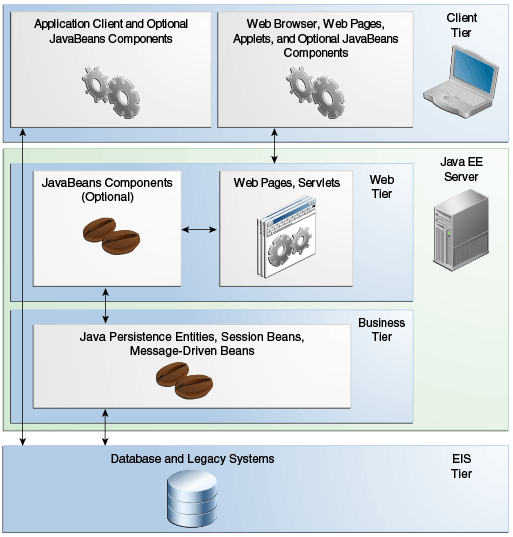
\includegraphics[width=\textwidth]{images/jakartaeett_dt_004}
    \label{img:jakartaee}
\end{figure}

\subsubsection{CDI}
Řízení životního cyklu samotné aplikace je často vhodné delegovat na nějaký framework, který je pro to většinou velmi dobře navržený. Kód, který je pak potřeba napsat, se v podstatě stává jakousi knihovnou pro tento framework. A přesně k tomuto účelu slouží právě CDI (Contexts and Dependency Injection).

\subsubsection{Jakarta Security 2.0}
V aplikaci jsem také musel řešit jak autentizaci, tak i autorizaci. Pro tyto účely jsem využil standard Jakarta Security 2.0, pro který má skvělou podporu aplikační server Payara, o kterém se zmiňuji dále. Konkrétně jsem využil JDBC Security realm, což je mechanismus, který umožňuje přímé propojení s databází a díky kterému je možné zabezpečit různé webové prostředky pouze za pomoci konfigurace (vizte příklad konfigurace \ref{lst:jakarta_security}). V té je možno mimo jiné nadefinovat například i různé role a jejich oprávnění, kam mohou přistupovat.

\begin{minipage}{\linewidth}
    \begin{lstlisting}[language=XML, label={lst:jakarta_security}, caption=Zjednodušený příklad Jakarta Security 2.0 konfigurace]
        <login-config>
            <auth-method>FORM</auth-method>
            <realm-name>onlineEduRealm</realm-name>
            <form-login-config>
                <form-login-page>/login.xhtml</form-login-page>
                <form-error-page>/login.xhtml</form-error-page>
            </form-login-config>
        </login-config>
        <security-role>
            <description>student</description>
            <role-name>student</role-name>
        </security-role>
        <security-constraint>
            <display-name>Student pages</display-name>
            <web-resource-collection>
                <web-resource-name>student</web-resource-name>
                <url-pattern>/student/*</url-pattern>
            </web-resource-collection>
            <auth-constraint>
                <role-name>student</role-name>
            </auth-constraint>
        </security-constraint>
    \end{lstlisting}
\end{minipage}


\subsubsection{JSF + Omnifaces}
Pro FE jsem použil technologii JSF (JavaServer Faces) spolu s Omnifaces. Ty dohromady nabízí velmi dobrou integraci s BE a také značně zrychlují vývoj díky přepřipraveným komponentám.
S čím vším JSF pracuje, je dobře vidět na obrázku \ref{img:jsf-architektura}. Co se týče životního cyklu požadavku na server, ten je přehledně vidět na obrázku \ref{img:jsf-life-cycle}.



\textit{JavaServer Faces (JSF) je frontendový framework, součást Jakarta EE.
Jeho účelem je výrazně zjednodušit vývoj a údržbu webových aplikací.
Konkrétně nabízí následující:}
\textit{
\begin{itemize}
    \item Umožňuje relativně snadno vytvořit uživatelské rozhraní ze znovu použitelných komponent.
    \item Zjednodušuje transport dat z aplikace do uživatelského rozhraní a zpět.
    \item Pomáhá spravovat stav mezi několika požadavky na server.
    \item Nabízí jednoduchý způsob provázání událostí generovaných u klienta s~kódem na serveru.
    \item Umožňuje vytvářet vlastní přepoužitelné komponenty. \emph{\cite{jakarta:jsf}}
\end{itemize}
}

\begin{figure}
    \caption{Zjednodušená architektura technologie JSF, převzato z \cite{goncalves_2013}}
    \centering
    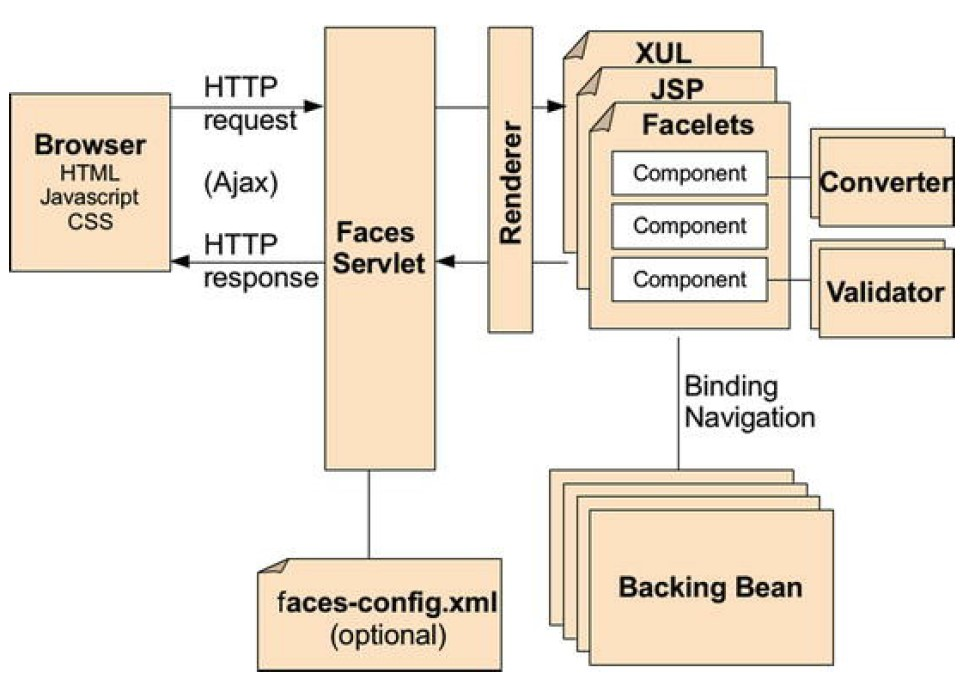
\includegraphics[width=\textwidth]{images/jsf-architektura}
    \label{img:jsf-architektura}
\end{figure}

\begin{figure}
    \caption{Životní cyklus JSF, převzato z \cite{goncalves_2013}}
    \centering
    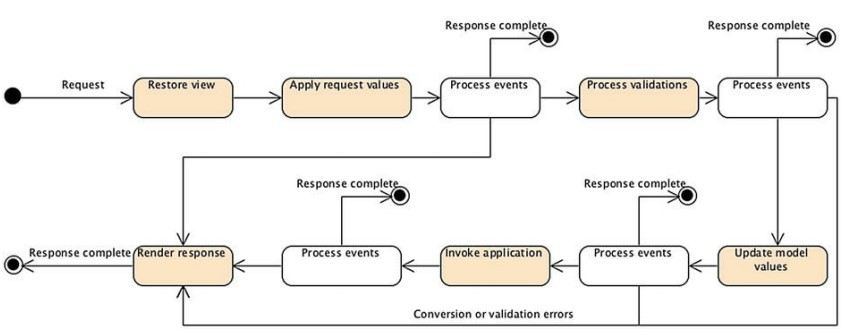
\includegraphics[width=\textwidth]{images/jsf-life-cycle}
    \label{img:jsf-life-cycle}
\end{figure}

\subsubsection{JPA}
Jelikož jsem se rozhodl pro relační databázi, tak je více než rozumné využít ORM (Objektově relační mapování). K tomu existuje v Jakarta EE standard JPA (Java Persistence API, od roku 2019 Jakarta Persistence).

Jedná se o standard, pomocí kterého lze s daty uložené v relační databázi pracovat jako s objekty. Programátor je tedy často odstíněn od psaní SQL skriptů.

\subsubsection{EJB}

\textit{\uv{EJB jsou serverové komponenty, které zapouzdřují byznys logiku a starají se o transakce, bezpečnost a další technické záležitosti, které by byly složité stále dokola implementovat. Řeší například vkládání závislostí, životní cyklus komponent, umožňují jednoduše definovat rozhraní pro webové služby a podobně. Samozřejmě jsou také velmi dobře integrované s dalšími Jakarta EE technologiemi, jako například JDBC, JPA, atd. Proto slouží mimo jiné jako vstupní bod k byznys logice například z JSF, tedy z prezentační vrstvy.}} \cite{goncalves_2013}

V praxi pak tedy stačí například označit třídu anotací \texttt{@Stateless} a je vyřešena spousta práce. Například se stane to, že všechny metody v této třídě budou vykonány jako samostatné transakce, což je ideální řešení například pro přístup k databázi.

\subsubsection{Jakarta WebSocket 2.0}
Při implementaci třídního chatu jsem řešil problém duplexní komunikace. Nakonec jsem k tomuto účelu použil Jakarta WebSocket 2.0. Jedná se o API specifikaci umožňující vývojáři do aplikace integrovat WebSockety. \cite{jakarta_websockets}


WebSocket je protokol umožňující perzistentní TCP spojení mezi serverem a klientem, takže si mohou data posílat libovolně. \cite{websockets}


\subsection{Primefaces}
Dále jsem využil knihovnu Primefaces verze 10. Ta nabízí spoustu předpřipravených konfigurovatelných komponent. Nějaké jsou samozřejmě již součástí JSF, nicméně Primefaces poskytují mnohem propracovanější řešení. Například u tabulek je možné nastavit různé filtrování, řazení, styly a podobně. Za zmínku stojí také například Richtext editor, který poskytuje v podstatě všechny důležité možnosti formátování a vkládání obrázků.

\subsection{PostgreSQL}
Pro ukládání dat jsem se rozhodl využít osvědčenou relační databázi PostgreSQL \cite{postgresql}. Hlavním důvodem je skvělá podpora ze strany Jakarta EE a také fakt, že nám tato technologie byla často doporučována během různých předmětů ve škole. Pro lepší práci s daty jsem využil ORM ve formě \uv{SQL to Code}. Jinými slovy jsem pomocí jazyka SQL nejprve vytvořil samotnou databázi a z té jsem posléze vygeneroval Java třídy včetně anotací. Tento přístup se mi zdál přirozenější jelikož jsem již znal základy jazyka SQL.

\subsection{Payara Server}
Jako aplikační server jsem zvolil Payara Server \cite{payara}, který vychází z GlassFish Server Open Source Edition. Hlavními důvody bylo, že je nabízen zdarma a má otevřený zdrojový kód. Navíc se snaží držet standardů.

\subsection{Docker}
Co se týče běhového prostředí, zde jsem se rozhodl pro kontejnerovou technologii Docker \cite{docker}. Ve stručnosti lze Docker chápat jako izolaci procesů. Narozdíl od klasické virtualizace tedy není potřeba virtualizovat celý operační systém, jelikož se využívá kernel samotného hostujícího OS. Důsledkem je to, že start takového kontejneru je téměř okamžitý a pro jeho běh je potřeba RAM a výpočetní prostředky pouze pro samotnou aplikaci, která je v něm izolována.

Konkrétně na produkčním prostředí běží celkem 2 kontejnery. A to Payara server se samotnou aplikací a dále PostgreSQL databáze.

\subsection{NGINX Reverse Proxy Server}
Pro zajištění https spojení jsem využil server NGINX Reverse Proxy \cite{nginx}. Samotnou konfiguraci reverzní proxy lze vidět v ukázce \ref{lst:reverse_proxy}.

\begin{minipage}{\linewidth}
    \begin{lstlisting}[language=XML, label={lst:reverse_proxy}, caption=Ukázka konfigurace reverzní proxy]
<IfModule mod_ssl.c>
	<VirtualHost *:443>
		ServerName online-edu.aubrecht.net
		ServerAdmin webmaster@localhost
		DocumentRoot /var/www/online-edu
		ErrorLog ${APACHE_LOG_DIR}/online-edu-error.log
		CustomLog ${APACHE_LOG_DIR}/online-edu-access.log combined
		ProxyPass / http://127.0.0.1:8780/
		ProxyPassReverse / http://127.0.0.1:8780/
		ProxyPassReverseCookieDomain 127.0.0.1 online-edu.aubrecht.net
		RewriteEngine on
		RewriteCond %{HTTP:Upgrade} websocket [NC]
		RewriteCond %{HTTP:Connection} Upgrade [NC]
		RewriteRule ^/omnifaces.push/(.*) "ws://127.0.0.1:8780/omnifaces.push/$1" [P,L]
		Header onsuccess edit Set-Cookie ^(.*)$ "$1; Secure"
		ProxyRequests off # Disable forward proxying
		SSLCertificateFile /etc/letsencrypt/live/online-edu.aubrecht.net/fullchain.pem
		SSLCertificateKeyFile /etc/letsencrypt/live/online-edu.aubrecht.net/privkey.pem
		Include /etc/letsencrypt/options-ssl-apache.conf
	</VirtualHost>
</IfModule>
    \end{lstlisting}
\end{minipage}

\section{Datový model}
Jako základní kámen, od kterého se následně odvíjely další činnosti, je datový model. Jedná se o souhrn entit, které v systému vystupují a vztahy mezi nimi.


\textit{\uv{Do určité míry lze na dobře sestavený datový model nahlížet jako na funkční
prototyp informačního systému, který budou později programátoři dělat.}}
\cite{merunka_vojtech_2006}

\begin{figure}
    \caption{Datový model}
    \centering
    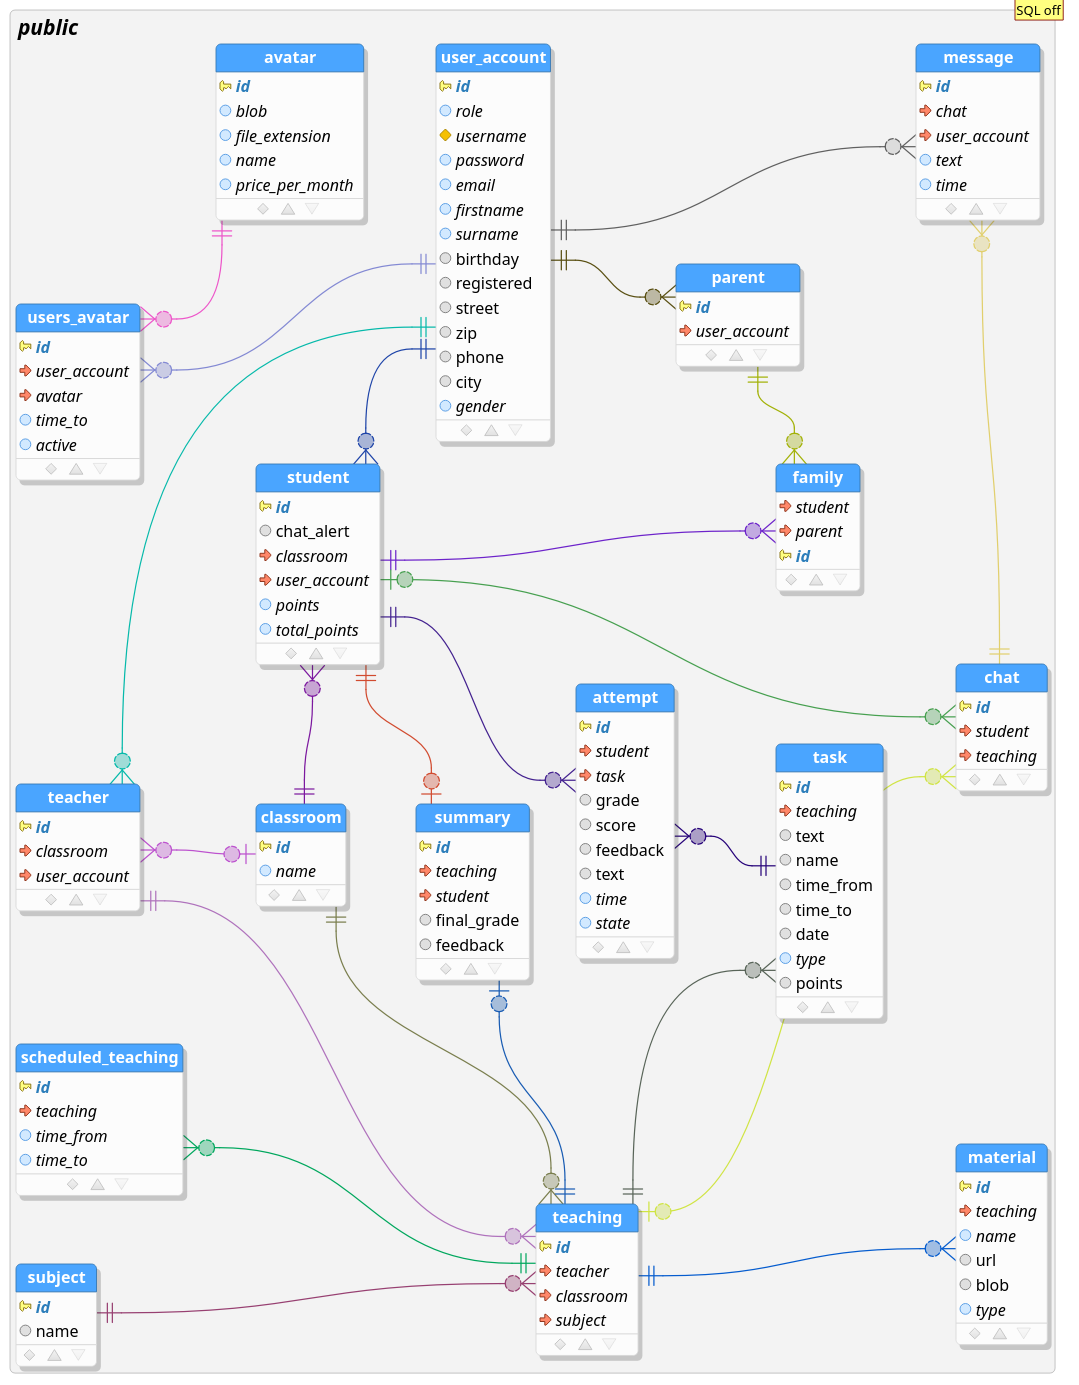
\includegraphics[width=\textwidth]{images/2021_04_14_datovy_model}
\end{figure}



\section{Stavový diagram úkolu}

Jednou z hlavních entit v systému je nepochybně samotný úkol, který učitel nebo učitelka zadává třídě k vypracování. Takový úkol může být buďto povinný a nebo dobrovolný za bonusové body. Ať už se jedná o jeden, či druhý typ úkolu, může se nacházet v různých stavech. Tyto stavy jsou vždy myšleny vzhledem ke konkrétnímu žákovi. Bylo by tedy možná přesnější říkat stav odevzdání konkrétního úkolu u konkrétního žáka. Aby tedy bylo možné rozhodnout stav tohoto úkolu ke konkrétnímu žákovi, je nutná nějaká třetí entita, která bude tento stav určovat. A tou je odeslaný pokus. Těch může žák k jednomu úkolu poslat hned několik, pokud je mu pokaždé vrácen k přepracování. Jakmile je některý z odeslaných pokusů učitelem schválen, tak je tím žákovi schválen celý úkol. Mimo to může vyučující žákovi úkol omluvit a to i v případě, že již vypršel termín odevzdání a žák má tento úkol již ve stavu nesplněný. Souhrnně tyto stavy vysvětluje diagram \ref{fig:taskStateDiagram}

\begin{figure}
    \caption{Stavový diagram úkolu}
    \centering
    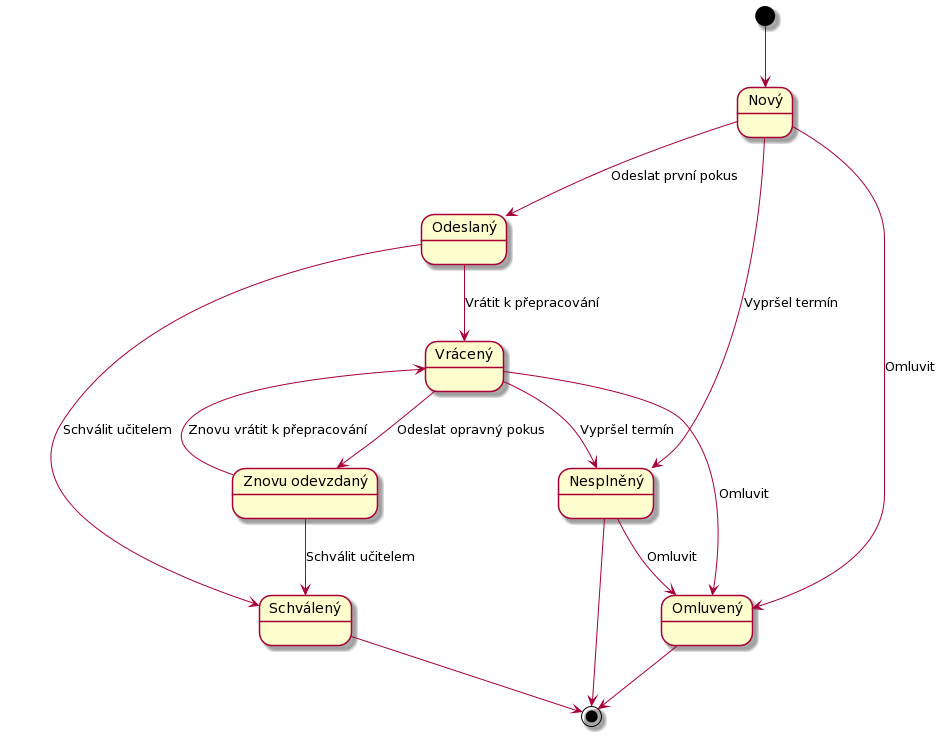
\includegraphics[width=\textwidth]{images/task-state-diagram}
    \label{fig:taskStateDiagram}
\end{figure}







\chapter{Gamifikace}
\label{chap:gamifikace}
Nad rámec zadání jsem se vynasnažil do systému dostat různé herní prvky. Důvodem je fakt, že se jedná o platformu určenou pro základní školy, a tak se jeví jako dobrý nápad tzv. Škola hrou, kterou prosazoval již Jan Amos Komenský. Cílem je tedy implementace různých zábavných a herních prvků, které by mohly děti motivovat k práci nenásilnou formou. 

Jako formu gamifikace jsem zvolil prvky detailně rozebrané v následujících podkapitolách.


\section{Body}
Úplným základem je získávání bodů za dobrovolná cvičení. Právě fakt, že je lze získat pouze za dobrovolné úkoly je velmi důležitý z psychologického hlediska. Pokud by totiž bylo možné získávat body za povinné úkoly pouze na základě toho, jak je jednotlivec chytrý, tak by to mohlo vést k pocitu marnosti u slabších jedinců.

Když je ovšem bude možné získat pouze za dobrovolné úkoly, tak to úplně mění situaci. To, že má někdo více bodů, pak totiž nemusí znamenat, že by byl chytřejší, ale spíše že je snaživější a dělá věci i navíc. 

\section{Žebříček}
Samotné body by byly víceméně k ničemu, kdyby neexistovalo nějaké srovnání mezi spolužáky, které by vyvolávalo soutěživost. Právě k tomuto účelu slouží třídní žebříček, kde se každý může podívat, kolik kdo získal bodů.

Rozhodně je ale potřeba třídě od začátku vysvětlovat, že zde má každý stejnou šanci a záleží pouze na snaze. A že i když se někdo na chvíli ocitne vespodu, nic mu nebrání dodělat nějaké starší cvičení a dostat se tak výše.

\section{Avatar}
Nakonec je opět z psychologického hlediska důležité i to, aby body prakticky k něčemu sloužily, například jako měna.

A tak vznikl nápad, že by žáci měli svého avatara, kterého by si za nasbírané body mohli vylepšovat. Takové vylepšení bude vždy na omezenou dobu, například 1 měsíc, aby stále existovala motivace pro průběžnou práci. Kdyby totiž žák získal všechny vylepšení příliš brzy, tak by pak mohl přestat pracovat.

Předměty, které si mohou žáci na svého avatara dokoupit mohou být velmi různorodé. Může se jednat například o ozdobné rámečky, brýle, čepice nebo klidně i celé, úplně nové avatary. Určitě je v této oblasti podle mého názoru obrovský potenciál, a rozhodně se tedy nebráním do budoucna spolupráci s grafikem či zapálenou komunitou. Příklad použitých avatarů lze vidět na obrázku \ref{img:avatars}.

\begin{figure}[]
    \caption{Ukázky avatarů, staženo pro nekomerční použití z \cite{pngegg}}
    \centering
    
\includegraphics[width=(0.25\textwidth)]{images/avatars/avatar-black.png}
    \hspace{0.1\textwidth}
    
\includegraphics[width=(0.25\textwidth)]{images/avatars/avatar-blue.png}
    \hspace{0.1\textwidth}
    
\includegraphics[width=(0.25\textwidth)]{images/avatars/avatar-green.png}
    
    
\includegraphics[width=(0.25\textwidth)]{images/avatars/avatar-lightblue.png}
    \hspace{0.1\textwidth}
    
\includegraphics[width=(0.25\textwidth)]{images/avatars/avatar-magenta.png}
    \hspace{0.1\textwidth}
    
\includegraphics[width=(0.25\textwidth)]{images/avatars/avatar-pink.png}
    \label{img:avatars}
\end{figure}

\section{Třídní chat}
Aby žák svého avatara někde využil a ukázal jej ostatním, implementoval jsem také třídní chat. Do toho mohou žáci a učitelé psát zprávy ozdobené vlastněným avatarem. Z technického hlediska se jedná o plnohodnotný chat s ukládáním zpráv do databáze. Také jsem rád, že jsem si zde vyzkoušel technologii WebSocket (vizte kapitolu \nameref{chap:architektura}).

\chapter{Uživatelské rozhraní}
V této sekci se nachází ukázky uživatelského rozhraní z již existující implementace.

\section{Přihlašovací obrazovka}
Přihlašování do systému probíhá pomocí uživatelského jména a hesla v jednoduchém formuláři. Roli uživatele pak systém rozpozná sám.
\begin{figure}[H]
    \caption{Přihlašovací obrazovka}
    \centering
    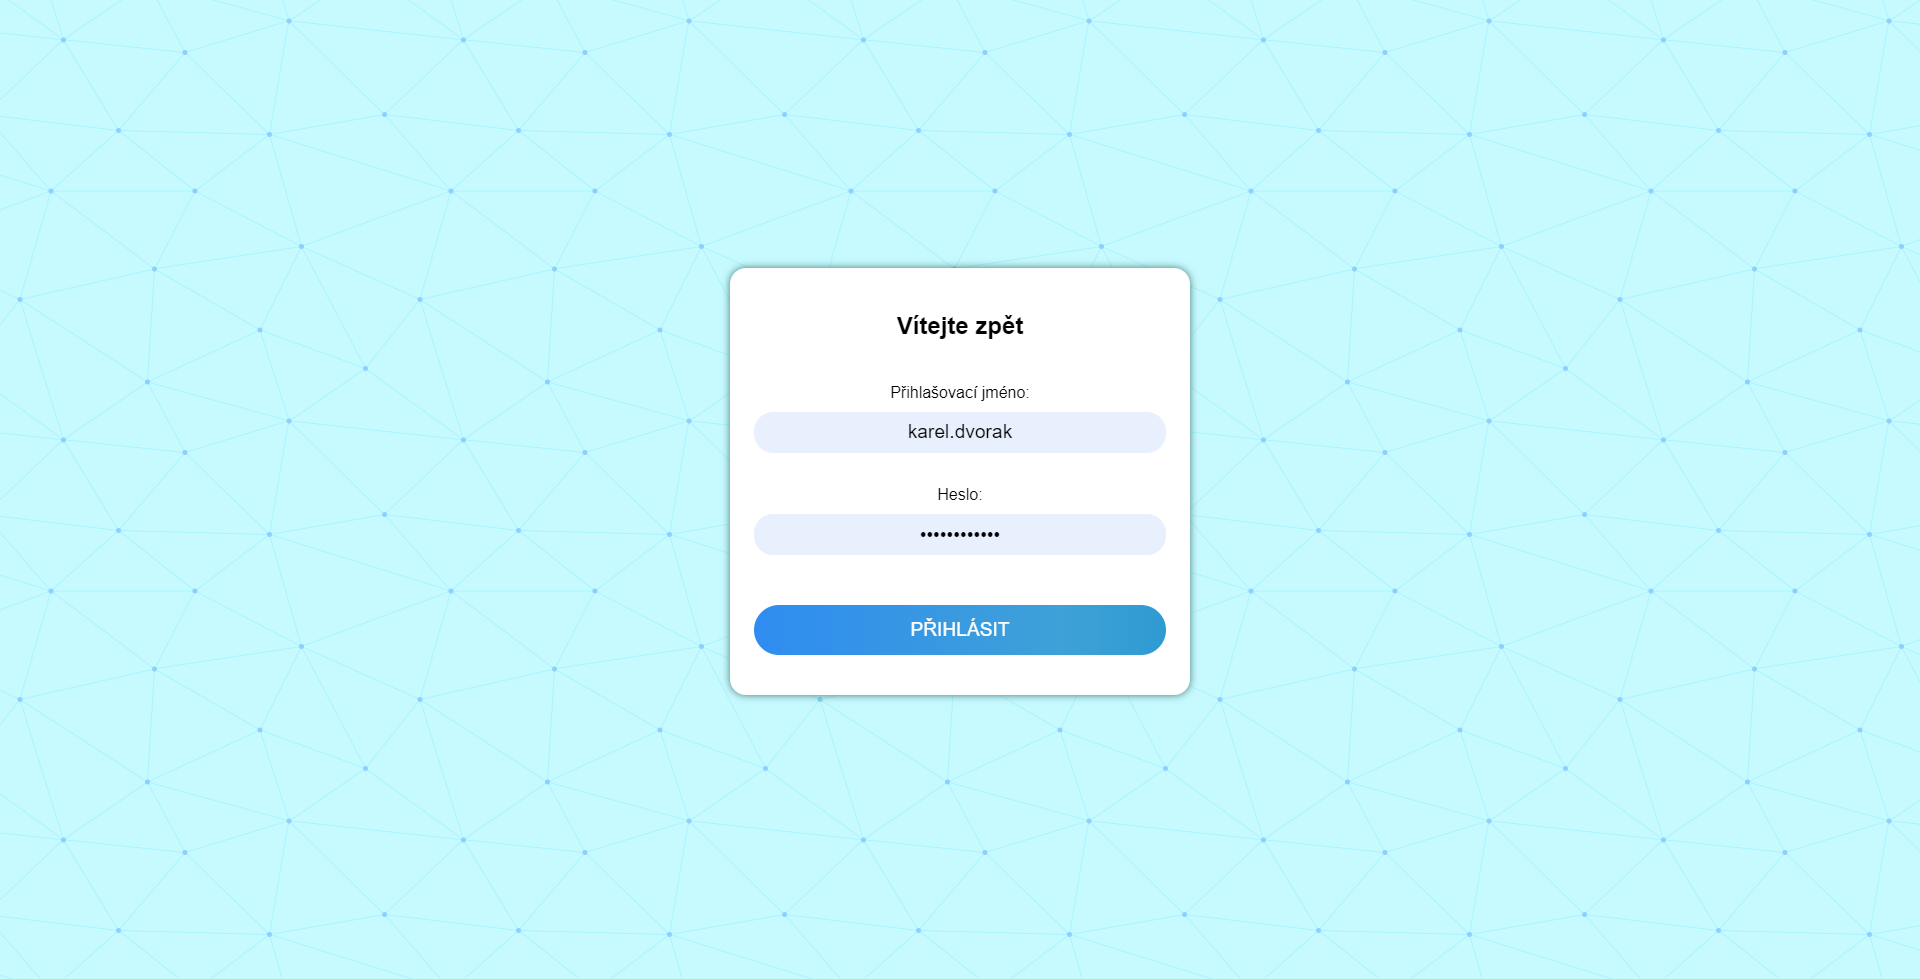
\includegraphics[width=\textwidth]{images/app_screenshots/login}
\end{figure}


\section{Rozhraní pro učitele}
Učitelské rozhraní nabízí snadné přepínání mezi třídami a vyučovanými předměty v dané třídě. Na obrázku \ref{ref:ucitel-seznam-ukolu} je pak konkrétně vidět seznam zadaných úkolů. Ty lze řadit podle různých sloupců a vytvářet úkoly nové. Každý z nich lze následně otevřít.
\begin{figure}[H]
    \caption{Učitel -- seznam úkolů}
    \label{ref:ucitel-seznam-ukolu}
    \centering
    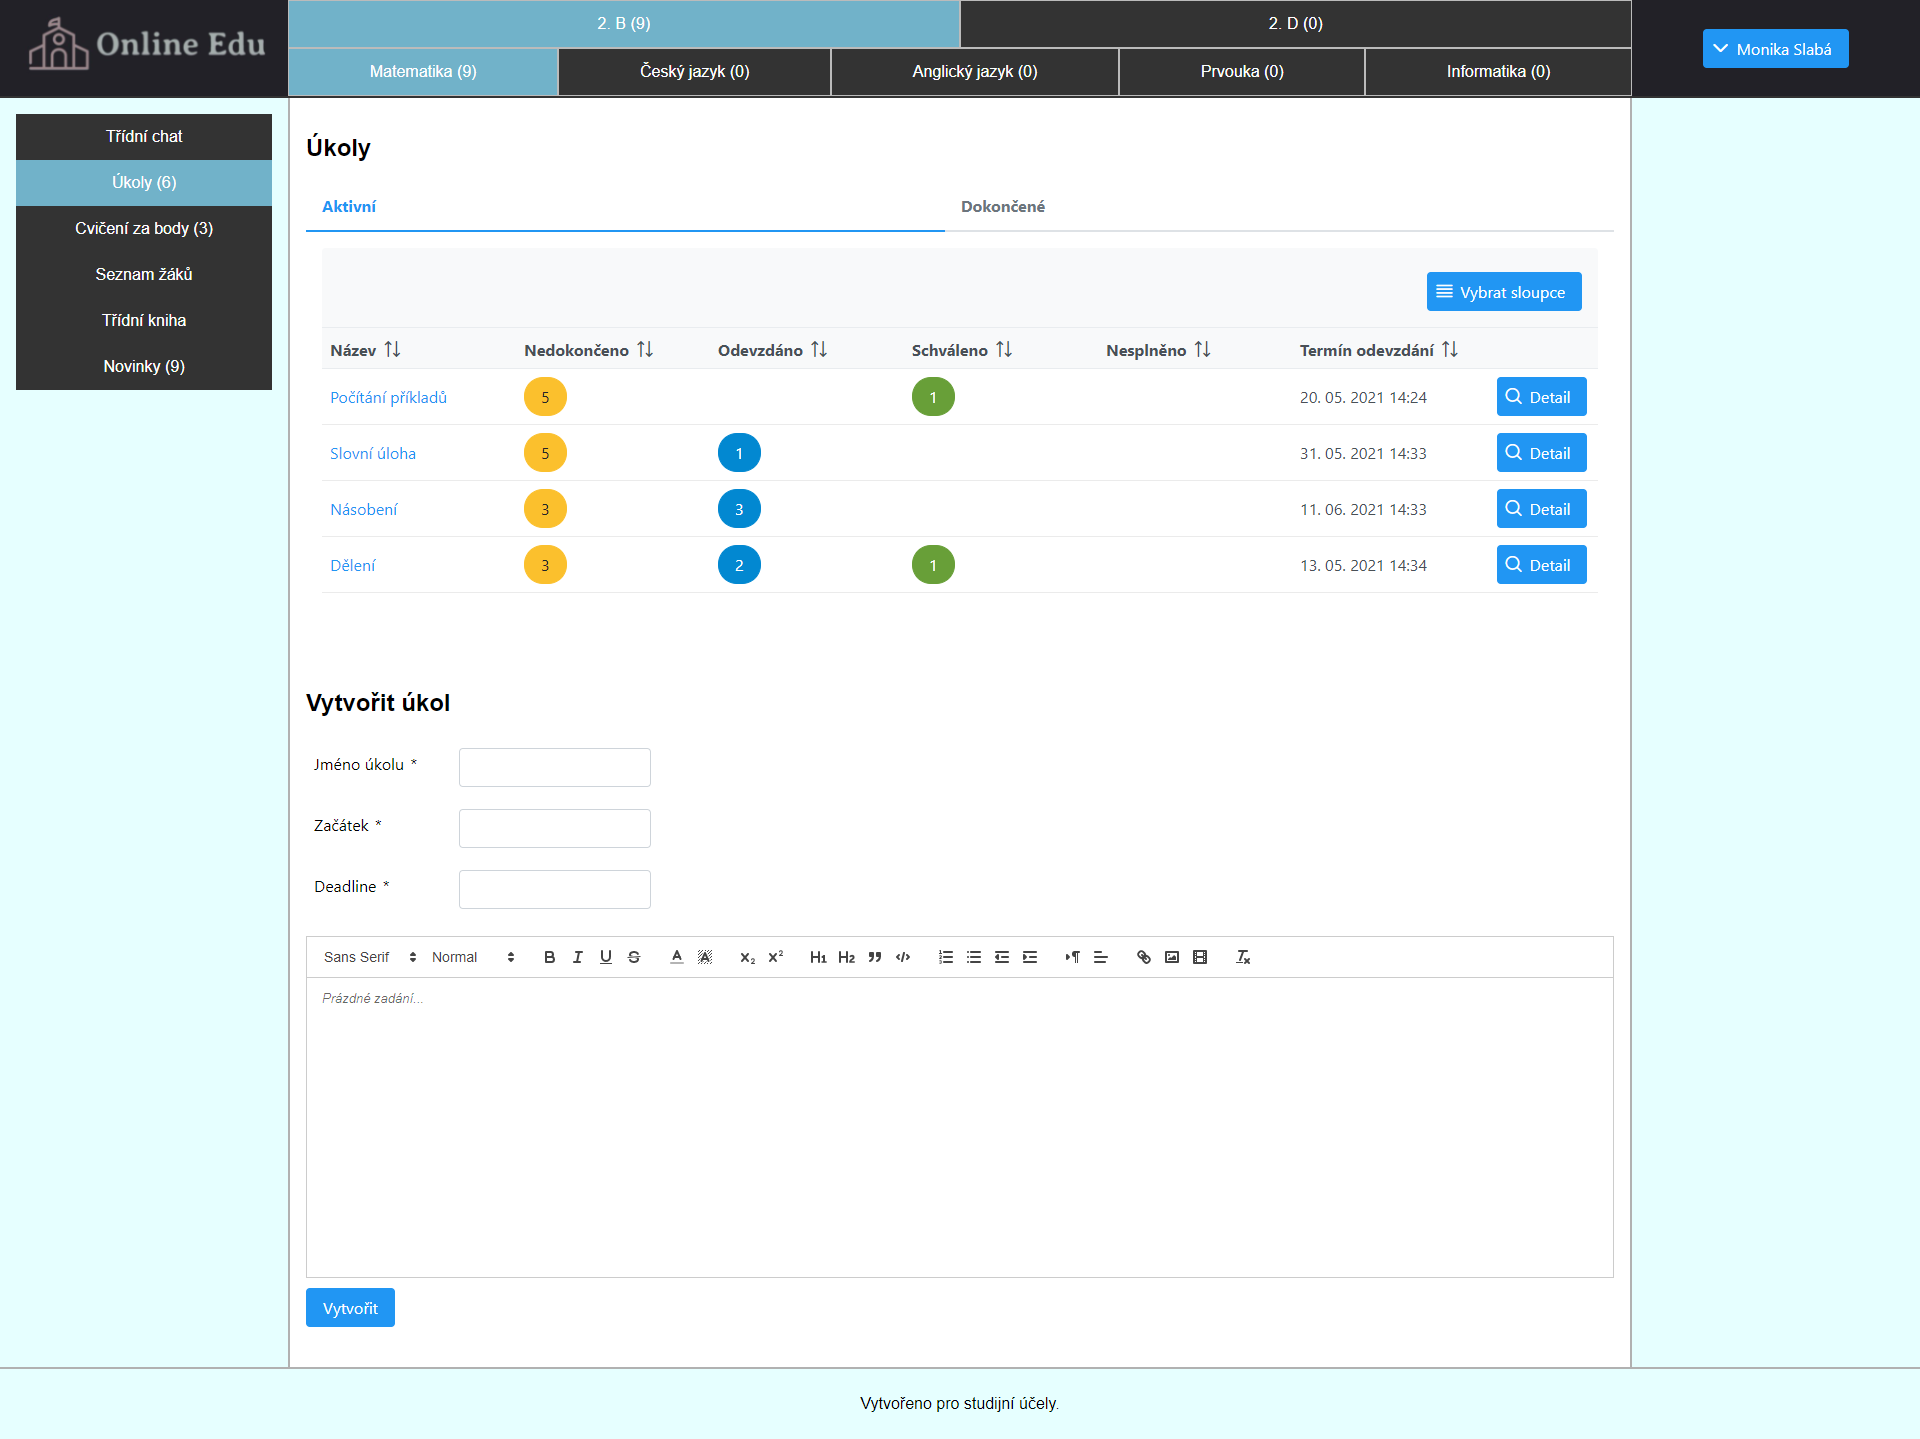
\includegraphics[width=\textwidth]{images/app_screenshots/ucitel_seznam_ukolu}
\end{figure}

Po otevření konkrétního úkolu se zobrazí jeho detail, jak je ukázáno na obrázku \ref{ref:ucitel-detail-ukolu}. Tam je pro každého žáka k dispozici seznam jeho pokusů, kde každý pokus lze opět otevřít.
\begin{figure}[H]
    \caption{Učitel -- detail úkolu}
    \label{ref:ucitel-detail-ukolu}
    \centering
    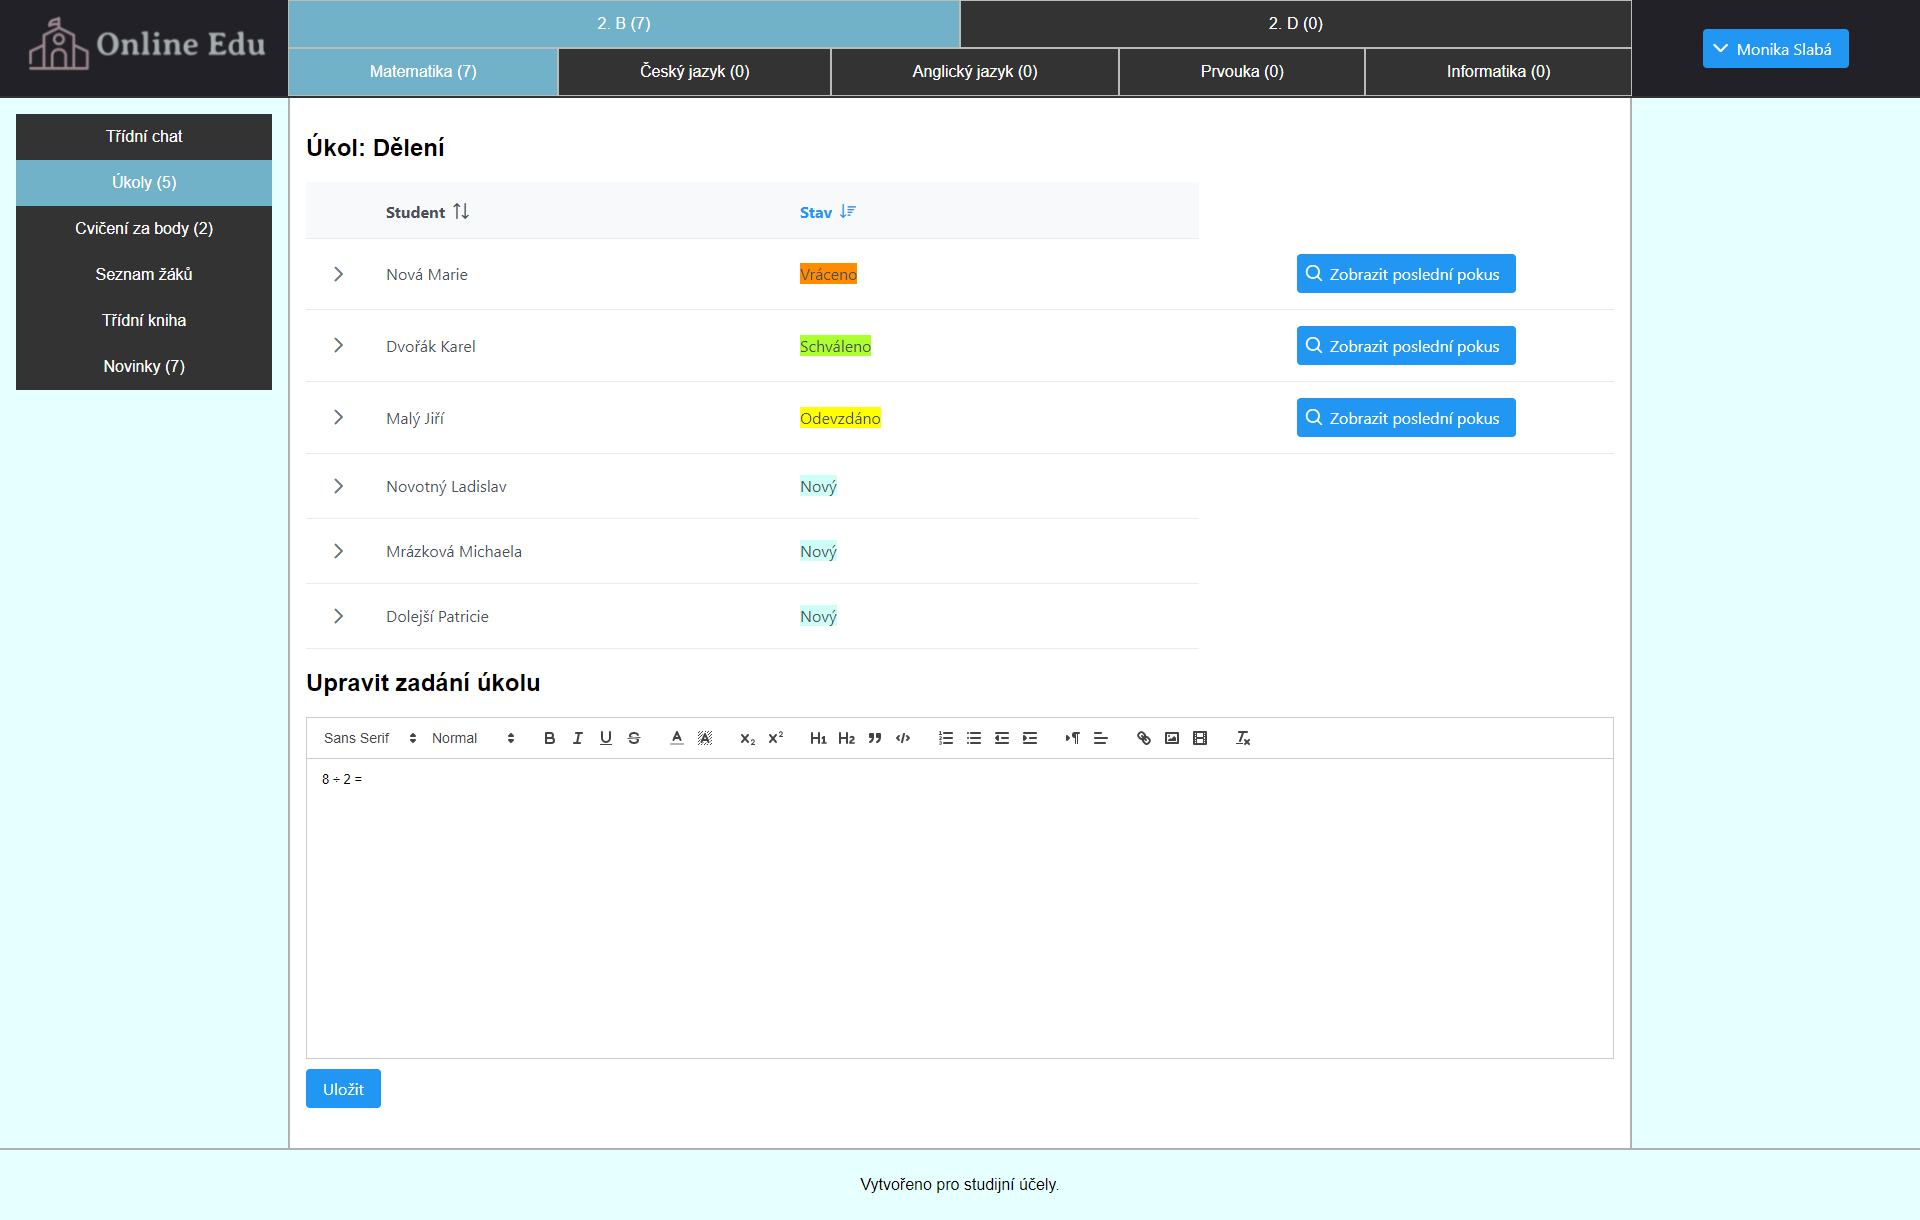
\includegraphics[width=\textwidth]{images/app_screenshots/ucitel_detail_ukolu}
\end{figure}

Na stránce detailu pokusu na obrázku \ref{ref:ucitel-detail-pokusu} lze vidět samotnou odpověď žáka a také prostor pro zpětnou vazbu. Tento pokus lze buďto schválit a tím schválit žákovi celý úkol nebo ho vrátit k přepracování.
\begin{figure}[H]
    \caption{Učitel -- detail pokusu}
    \label{ref:ucitel-detail-pokusu}
    \centering
    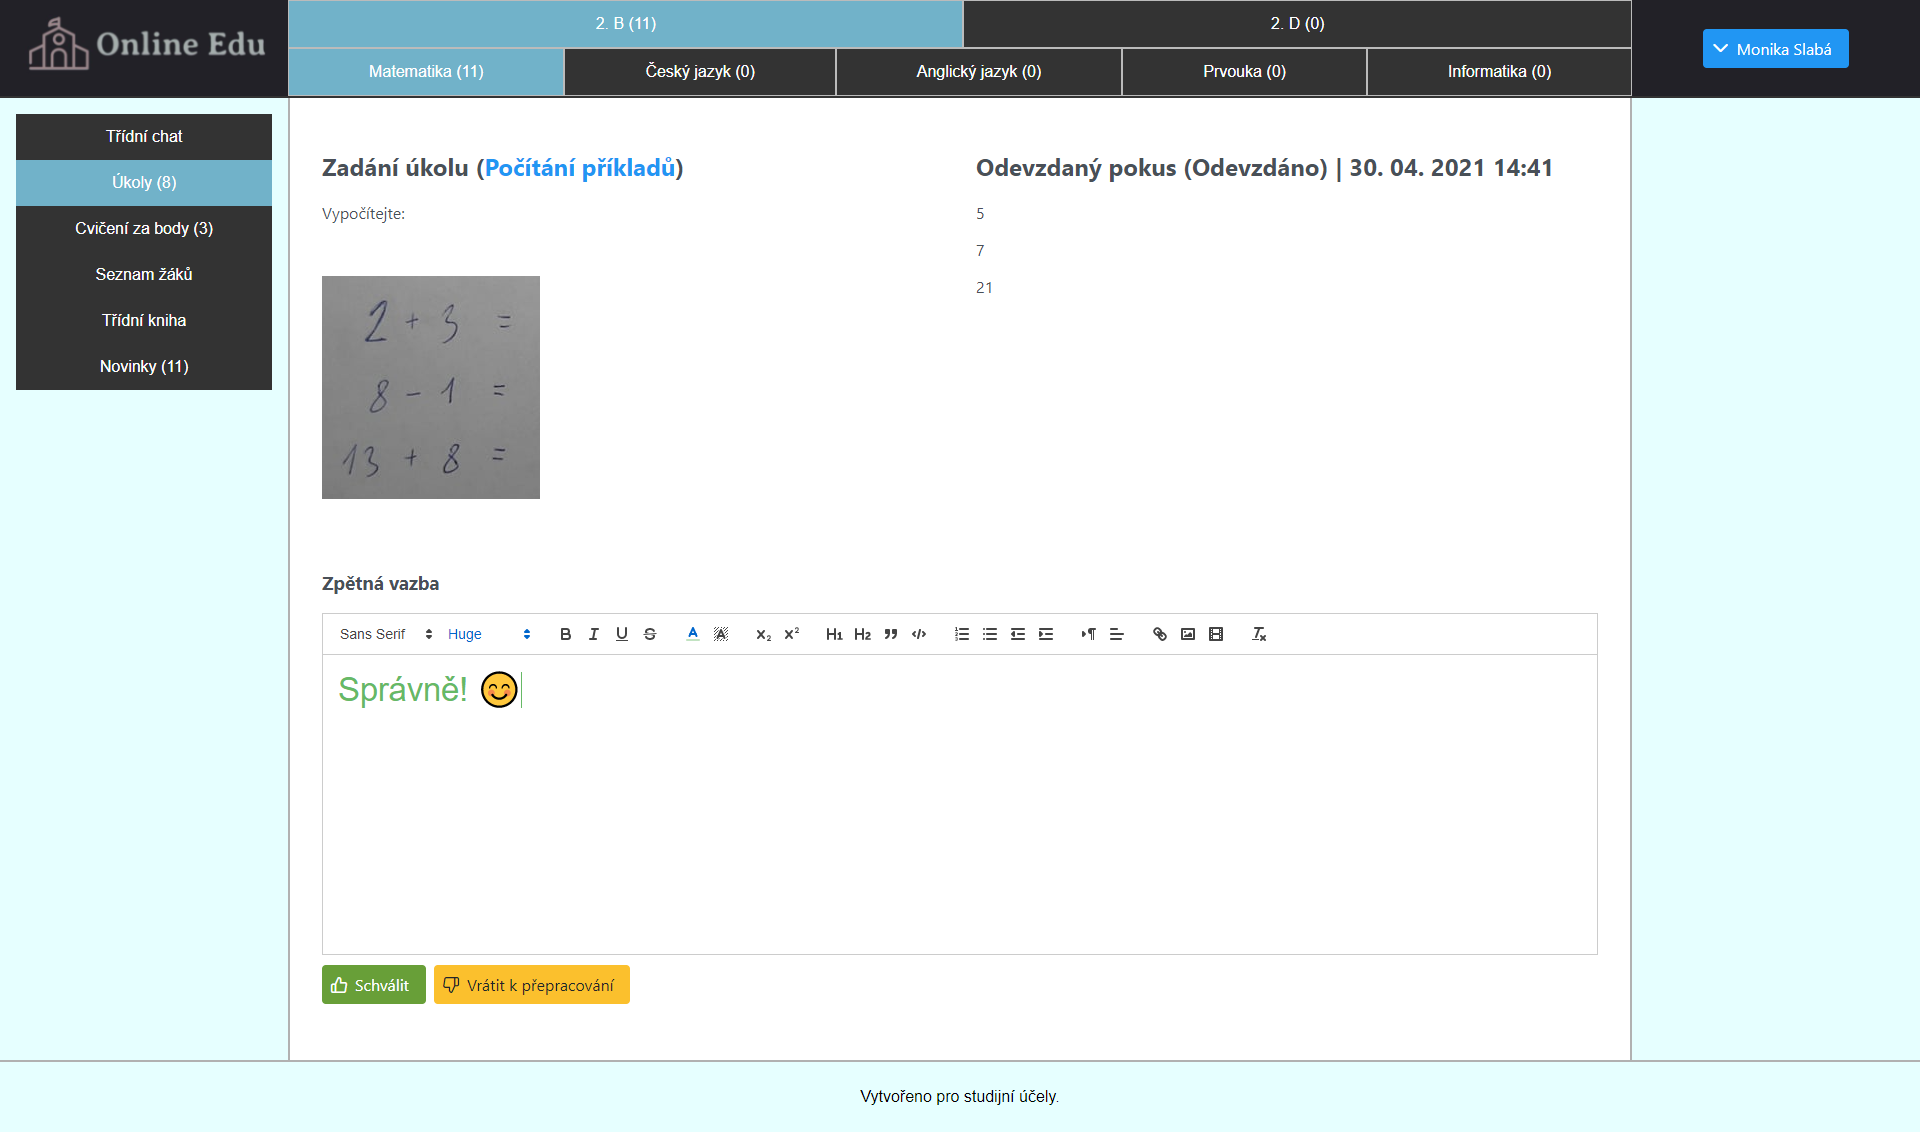
\includegraphics[width=\textwidth]{images/app_screenshots/ucitel_schvaleni_pokusu.png}
\end{figure}

Na obrázku \ref{ref:ucitel-chat} je vidět třídní chat. Ten vypadá stejně z pohledu žáka i učitele.
\begin{figure}[H]
    \caption{Učitel -- chat}
    \label{ref:ucitel-chat}
    \centering
    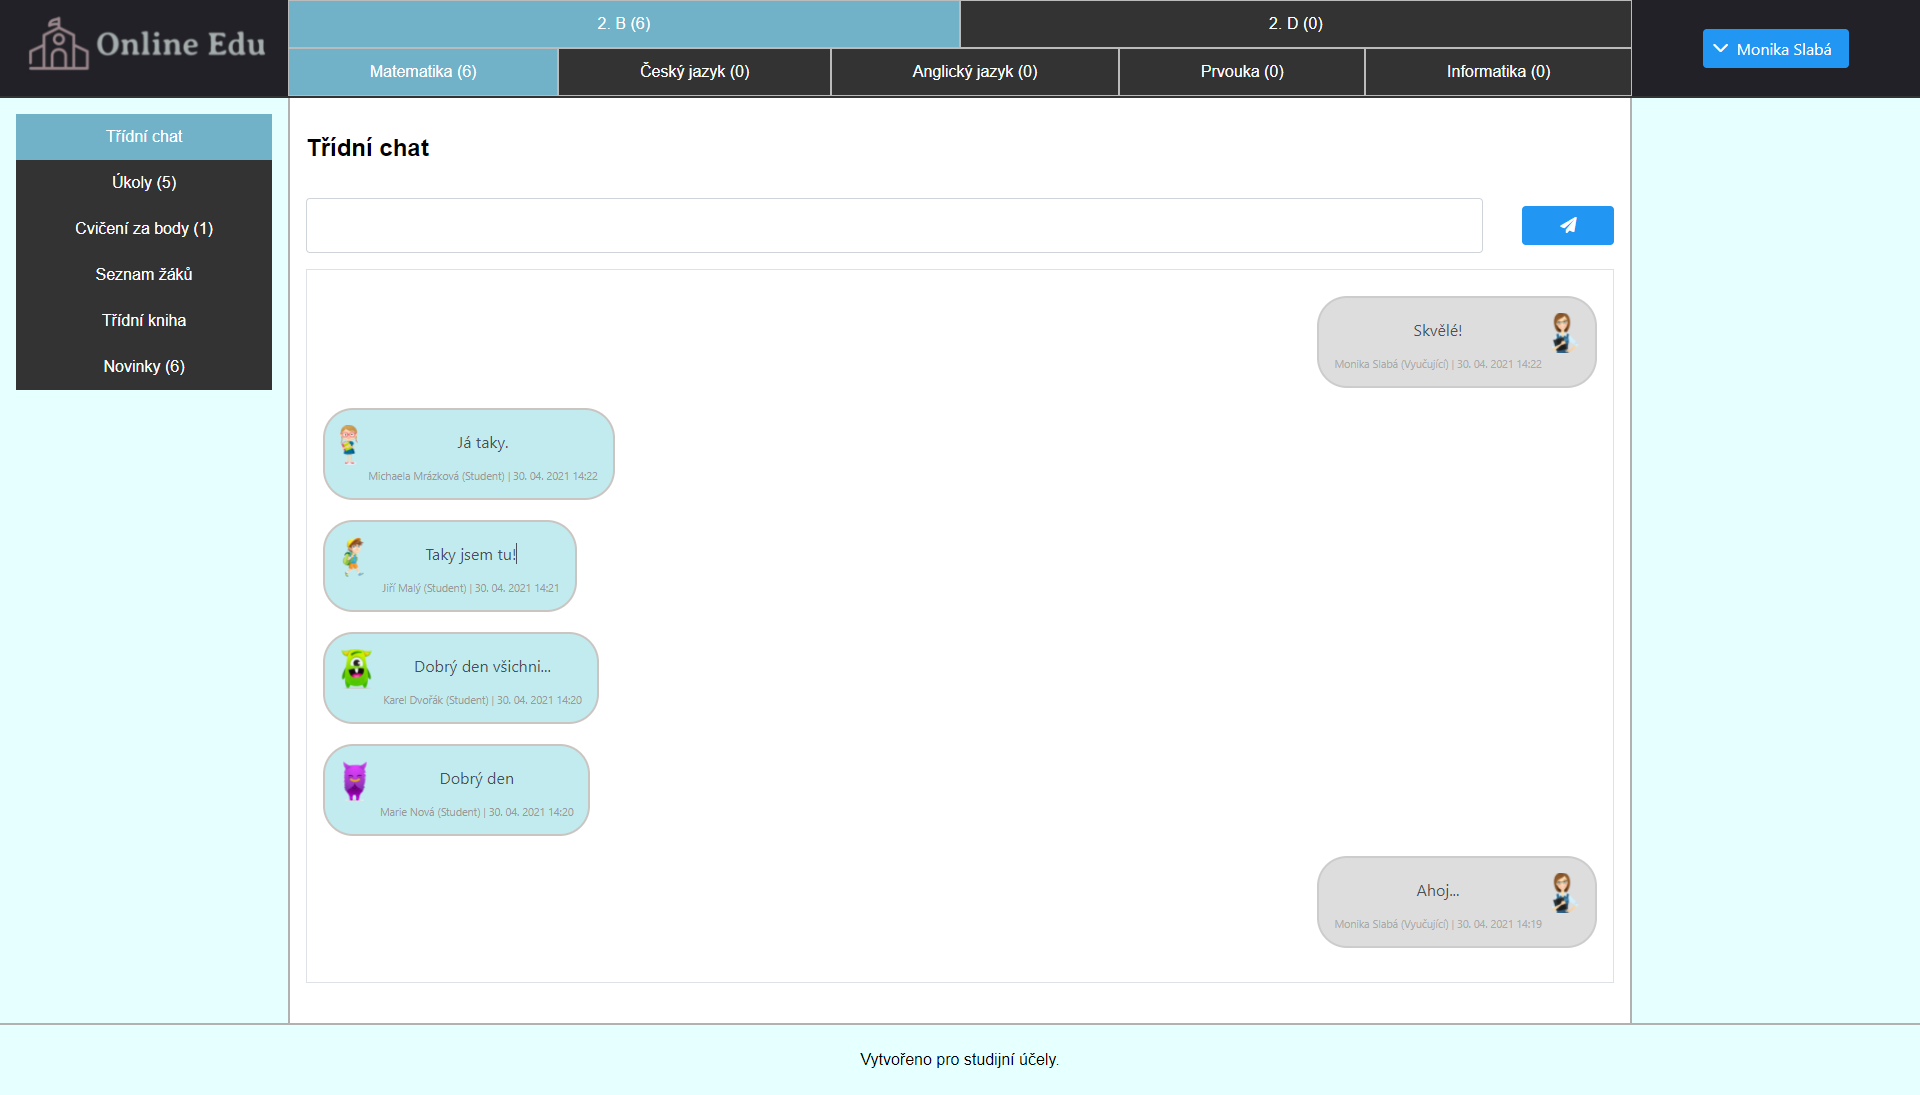
\includegraphics[width=\textwidth]{images/app_screenshots/ucitel_chat_avatari}
\end{figure}

Učitel si také může například měnit své heslo na stránce svého profilu na obrázku \ref{ref:ucitel-profil}.
\begin{figure}[H]
    \caption{Učitel -- profil}
    \label{ref:ucitel-profil}
    \centering
    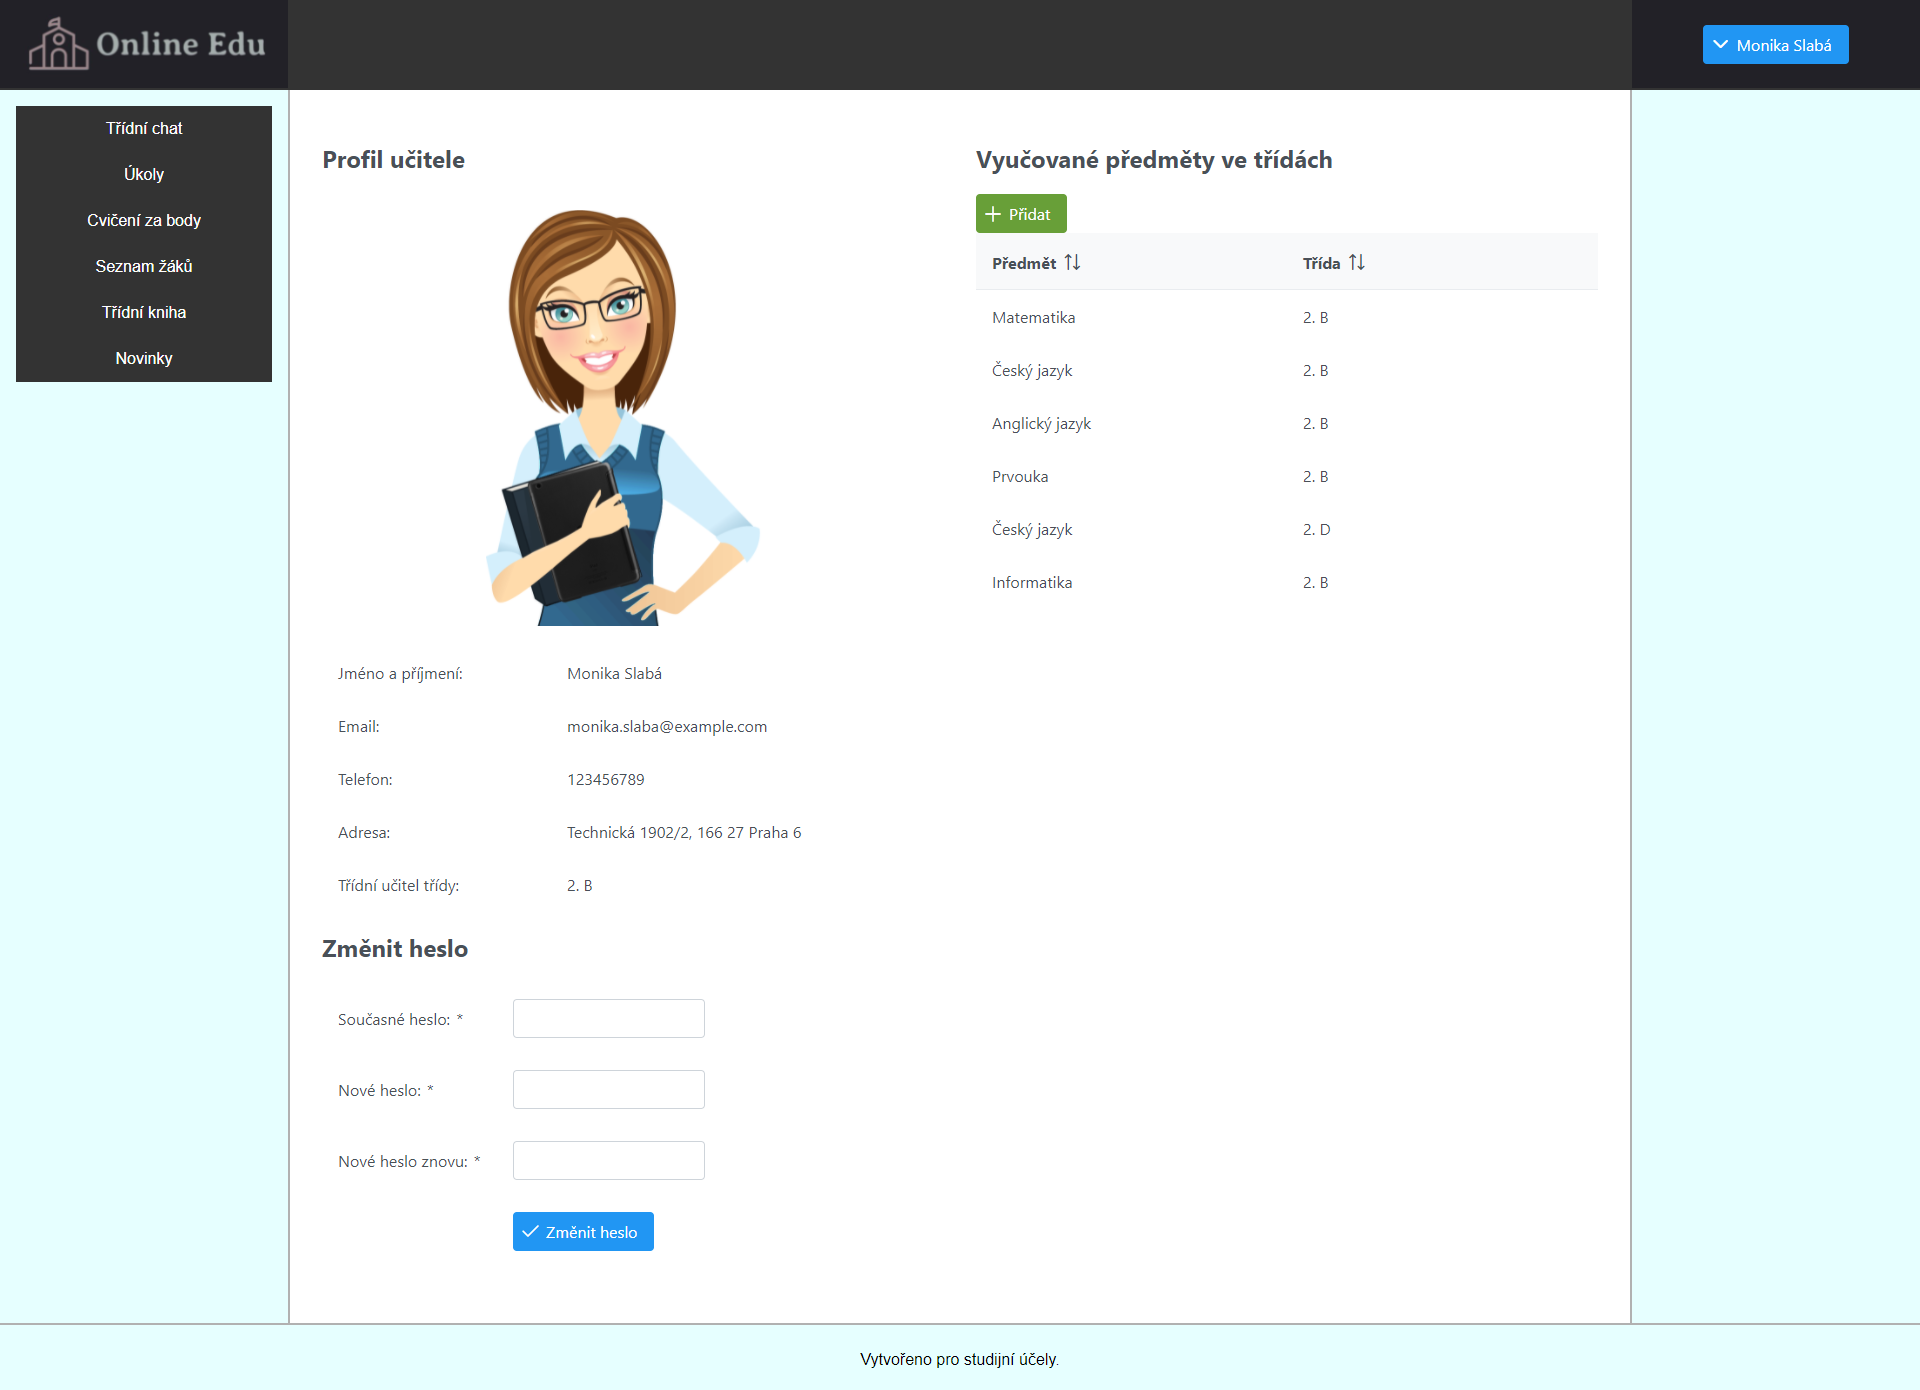
\includegraphics[width=\textwidth]{images/app_screenshots/ucitel_profil}
\end{figure}


\section{Rozhraní pro žáky}

Žákovské rozhraní se velmi podobá tomu učitelskému, jen nabízí jiné funkce. Například žák je fixně ve své třídě a může přepínat jen mezi svými předměty. Konkrétně na stránce seznam úkolů na obrázku \ref{ref:student-seznam-ukolu} vidí seznam všech úkolů v daném předmětu, kde na každý může kliknout a zobrazit si jeho detail.
\begin{figure}[H]
    \caption{Student -- seznam úkolů}
    \label{ref:student-seznam-ukolu}
    \centering
    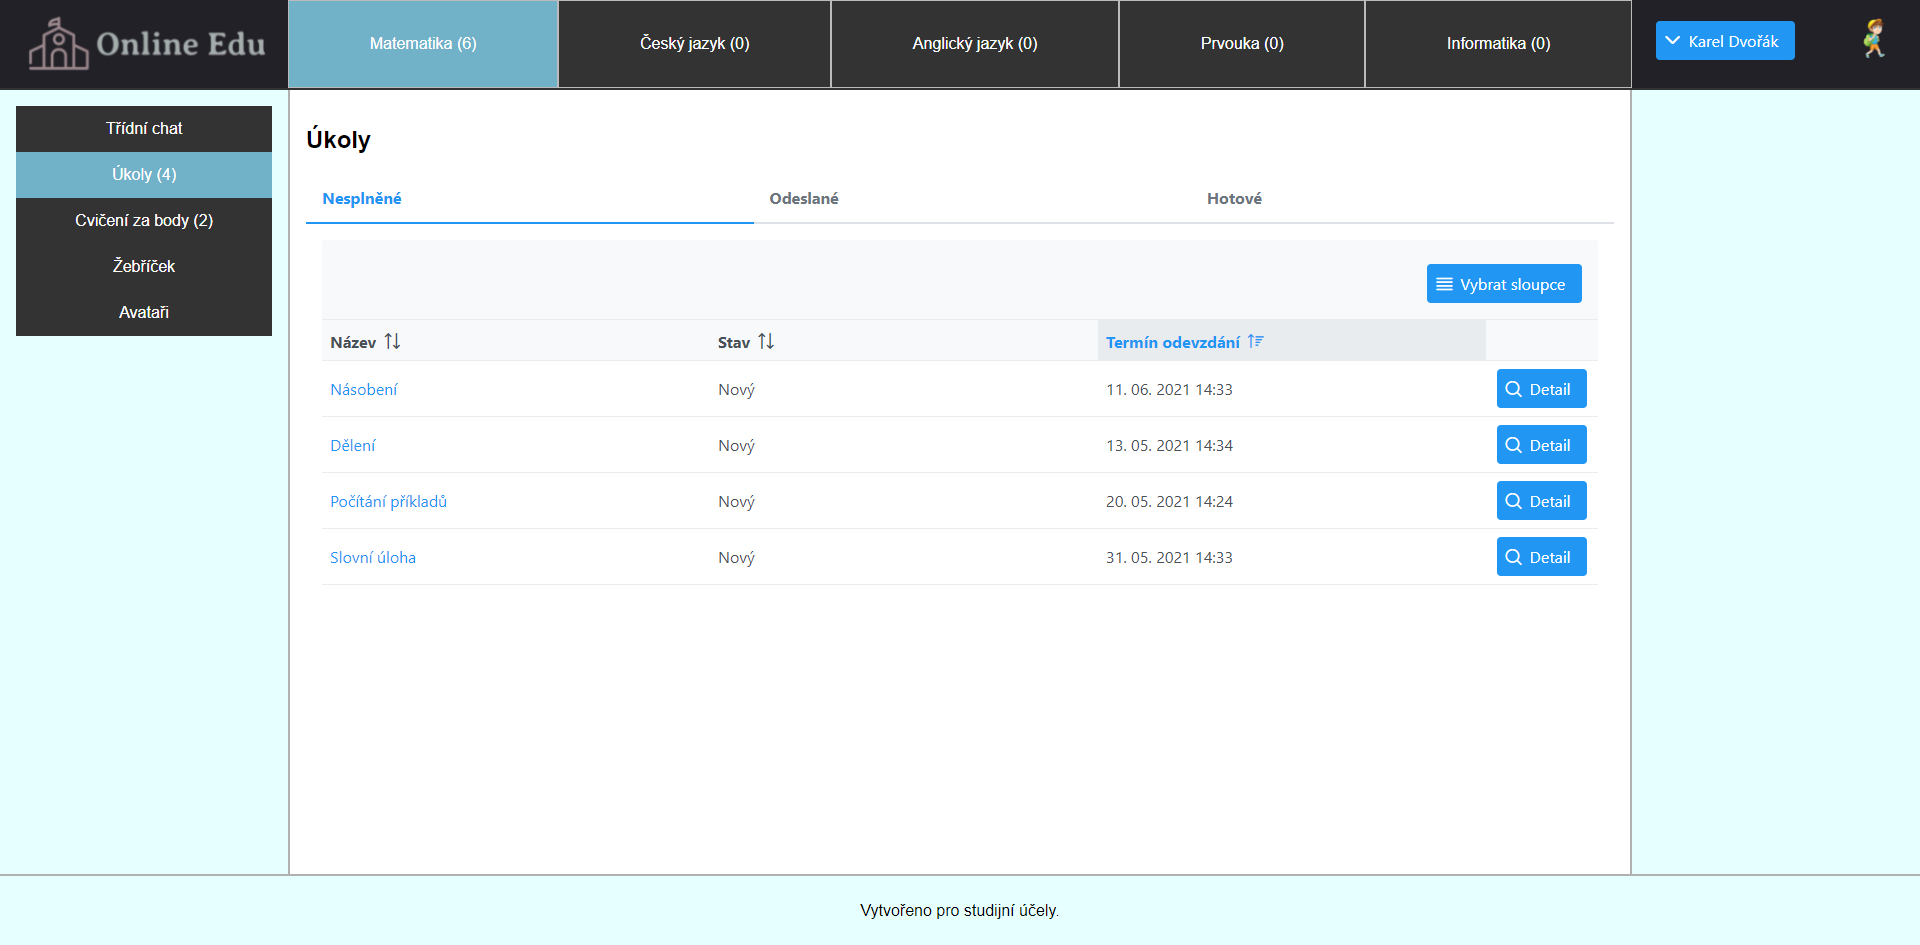
\includegraphics[width=\textwidth]{images/app_screenshots/zak_nove_ukoly}
\end{figure}

Po zobrazení detailu úkolu k němu může odeslat řešení jak je vidět na obrázku \ref{ref:student-novy-pokus}.
\begin{figure}[H]
    \caption{Student -- nový pokus}
    \label{ref:student-novy-pokus}
    \centering
    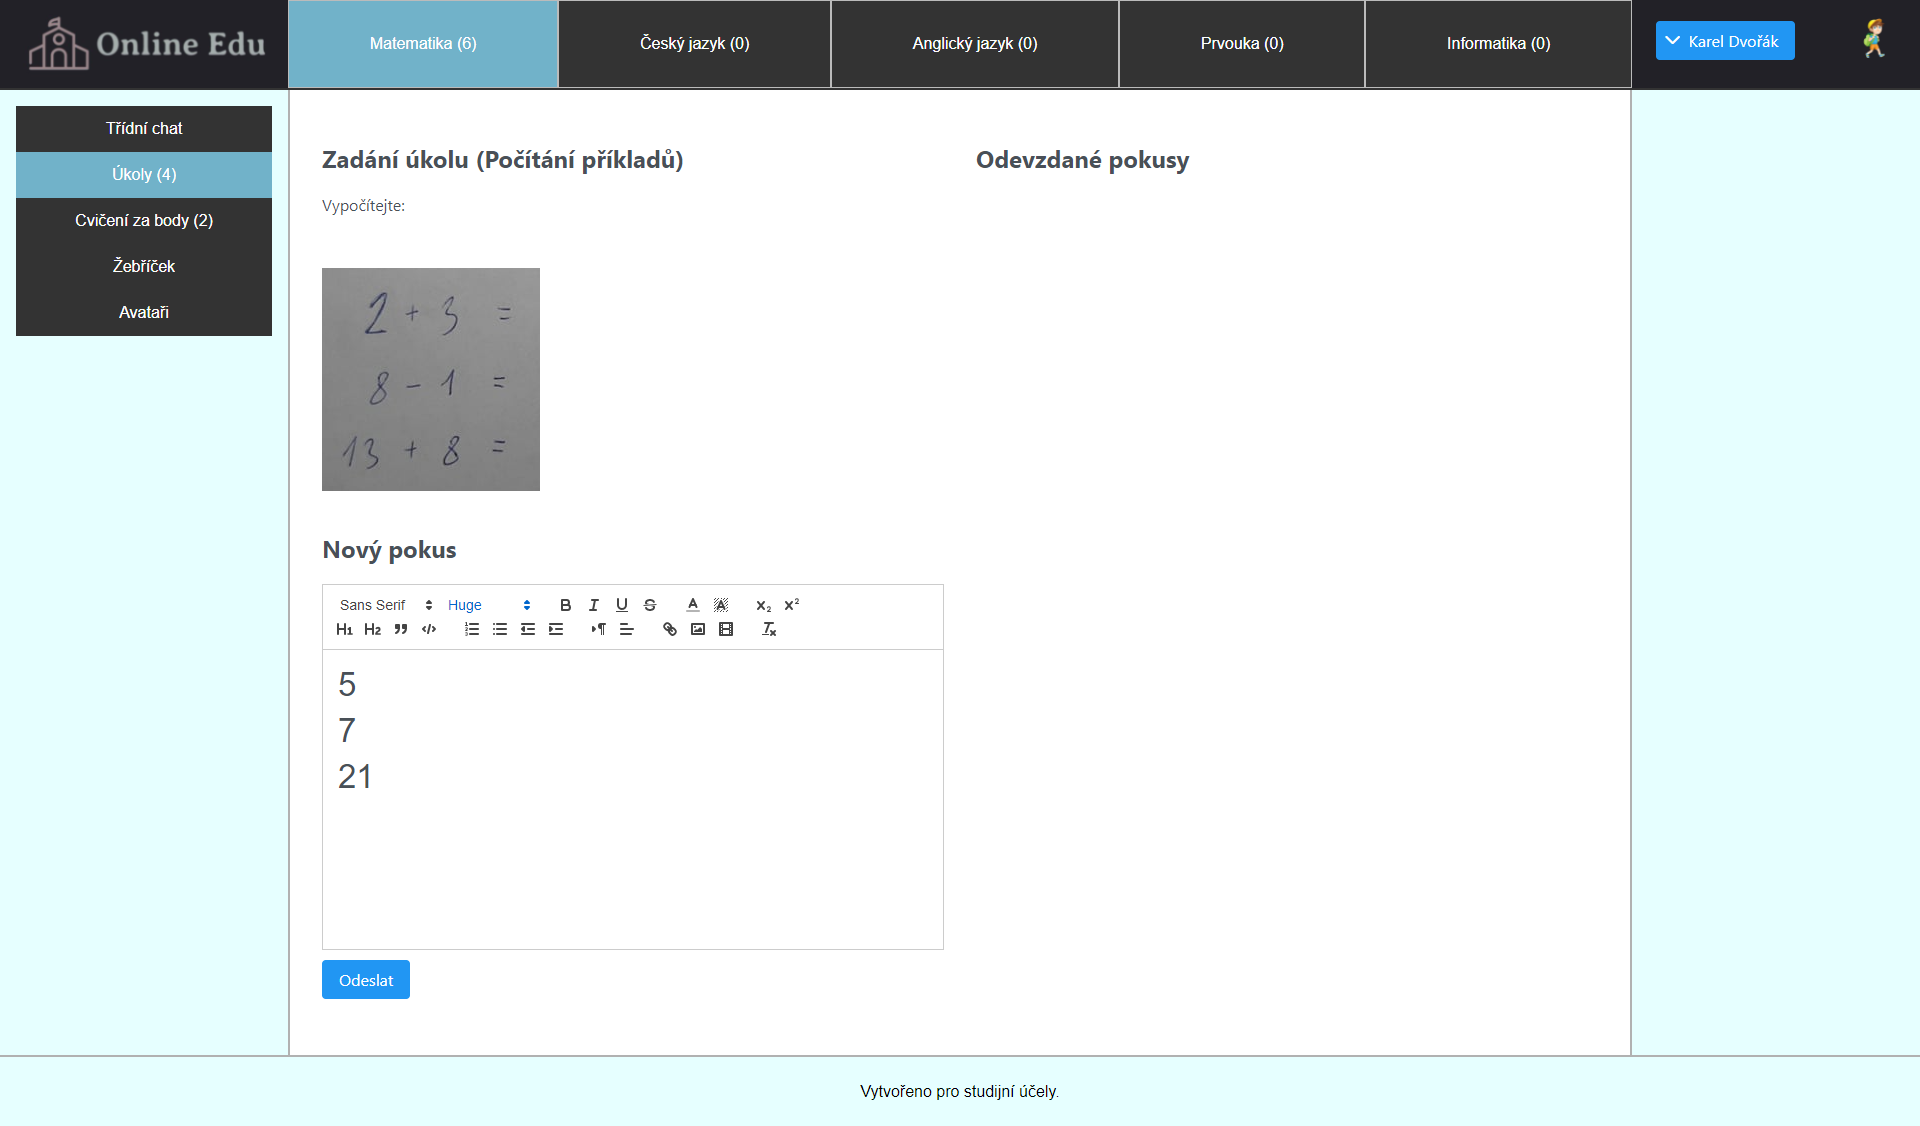
\includegraphics[width=\textwidth]{images/app_screenshots/zak_novy_pokus}
\end{figure}

Jak vidí žák detail schváleného úkolu je vidět na obrázku \ref{ref:student-schvaleny-ukol}. Nemá zde již možnost posílat další pokusy a v pravé části vidí náhledy odeslaných pokusů včetně zpětné vazby.
\begin{figure}[H]
    \caption{Student -- schválený úkol}
    \label{ref:student-schvaleny-ukol}
    \centering
    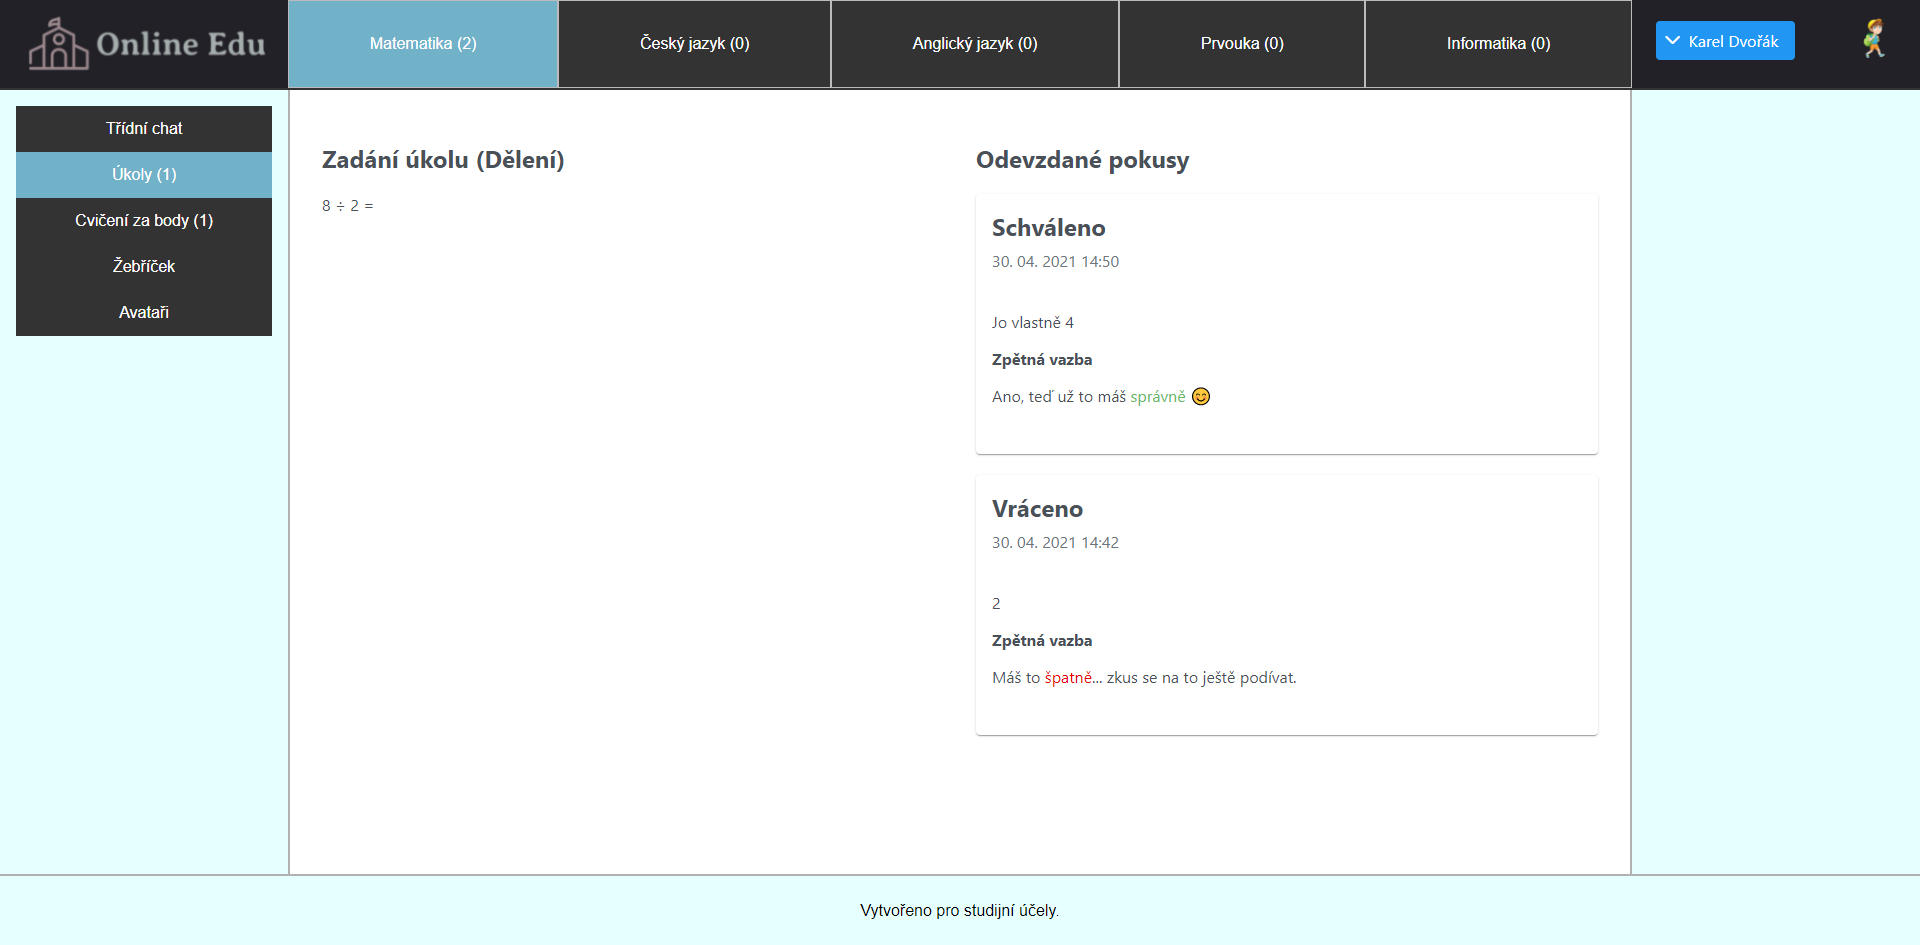
\includegraphics[width=\textwidth]{images/app_screenshots/zak_schvaleny_ukol}
\end{figure}


Jak popisuji v kapitole \ref{chap:gamifikace}, rozhodl jsem se do systému nad rámec řešení implementovat gamifikační prvky. S tím souvisí nakupování avatarů na obrázku \ref{ref:student-avatari}, kde si žák může za své body kupovat avatary a následně si volit, kterého chce zrovna používat. S tím také souvisí třídní žebříček, kde si může žák prohlédnout avatary svých spolužáků na obrázku \ref{ref:student-zebricek}
\begin{figure}[H]
    \caption{Student -- avataři}
    \label{ref:student-avatari}
    \centering
    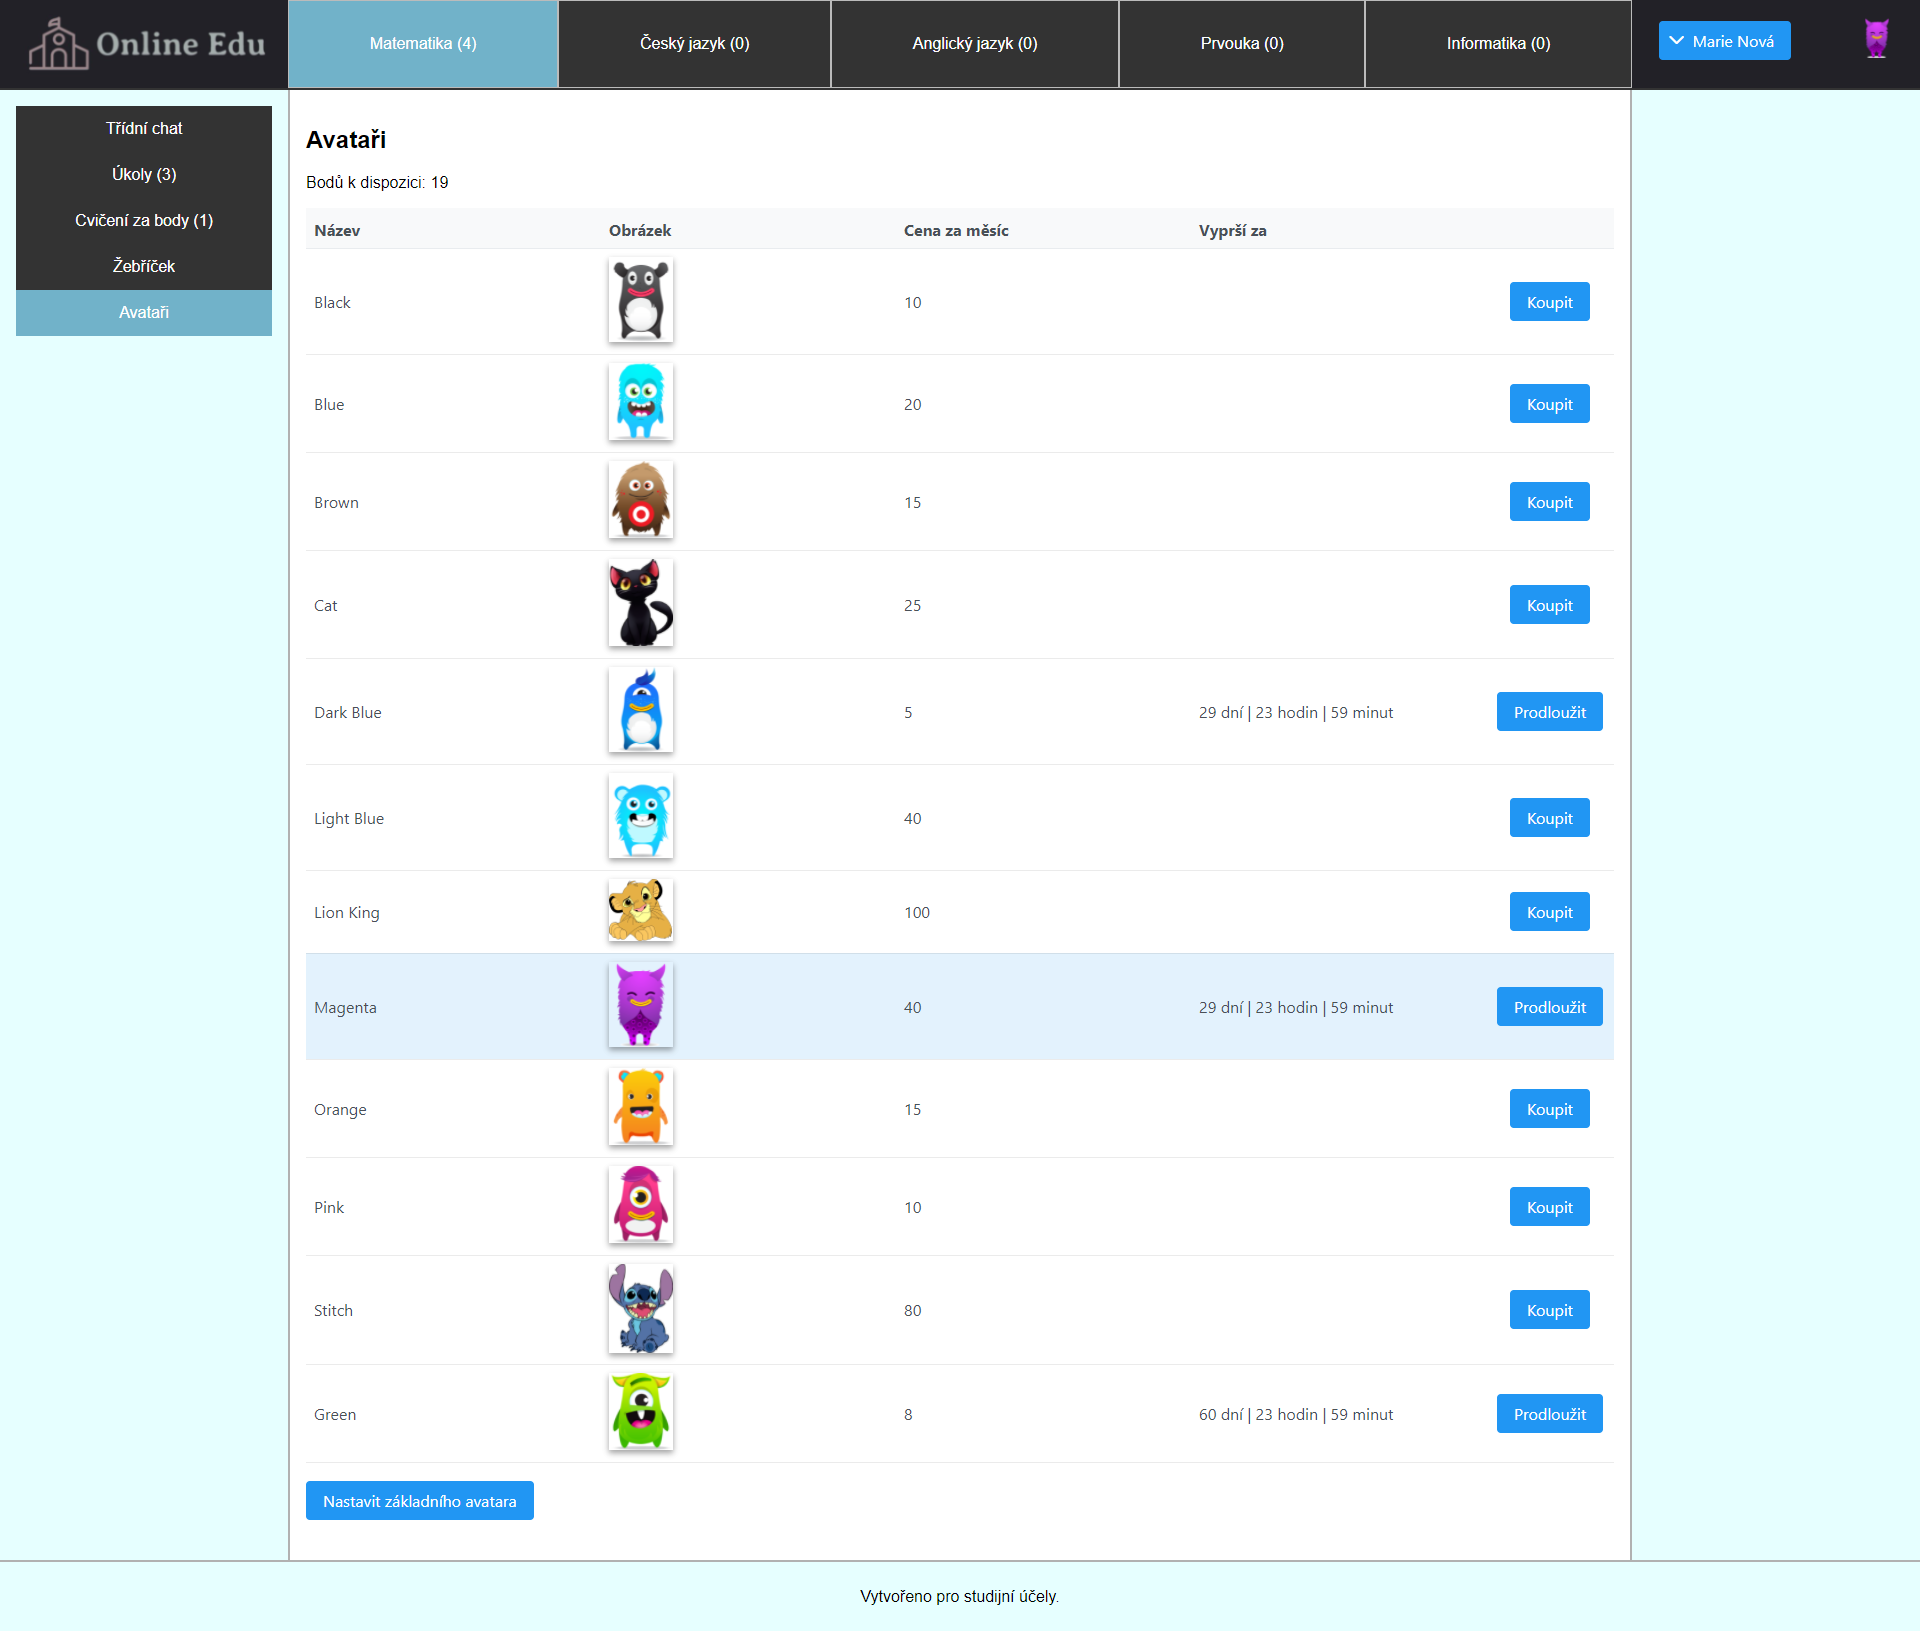
\includegraphics[width=\textwidth]{images/app_screenshots/zak_seznam_avataru_vybrany_2}
\end{figure}
\begin{figure}[H]
    \caption{Student -- žebříček}
    \label{ref:student-zebricek}
    \centering
    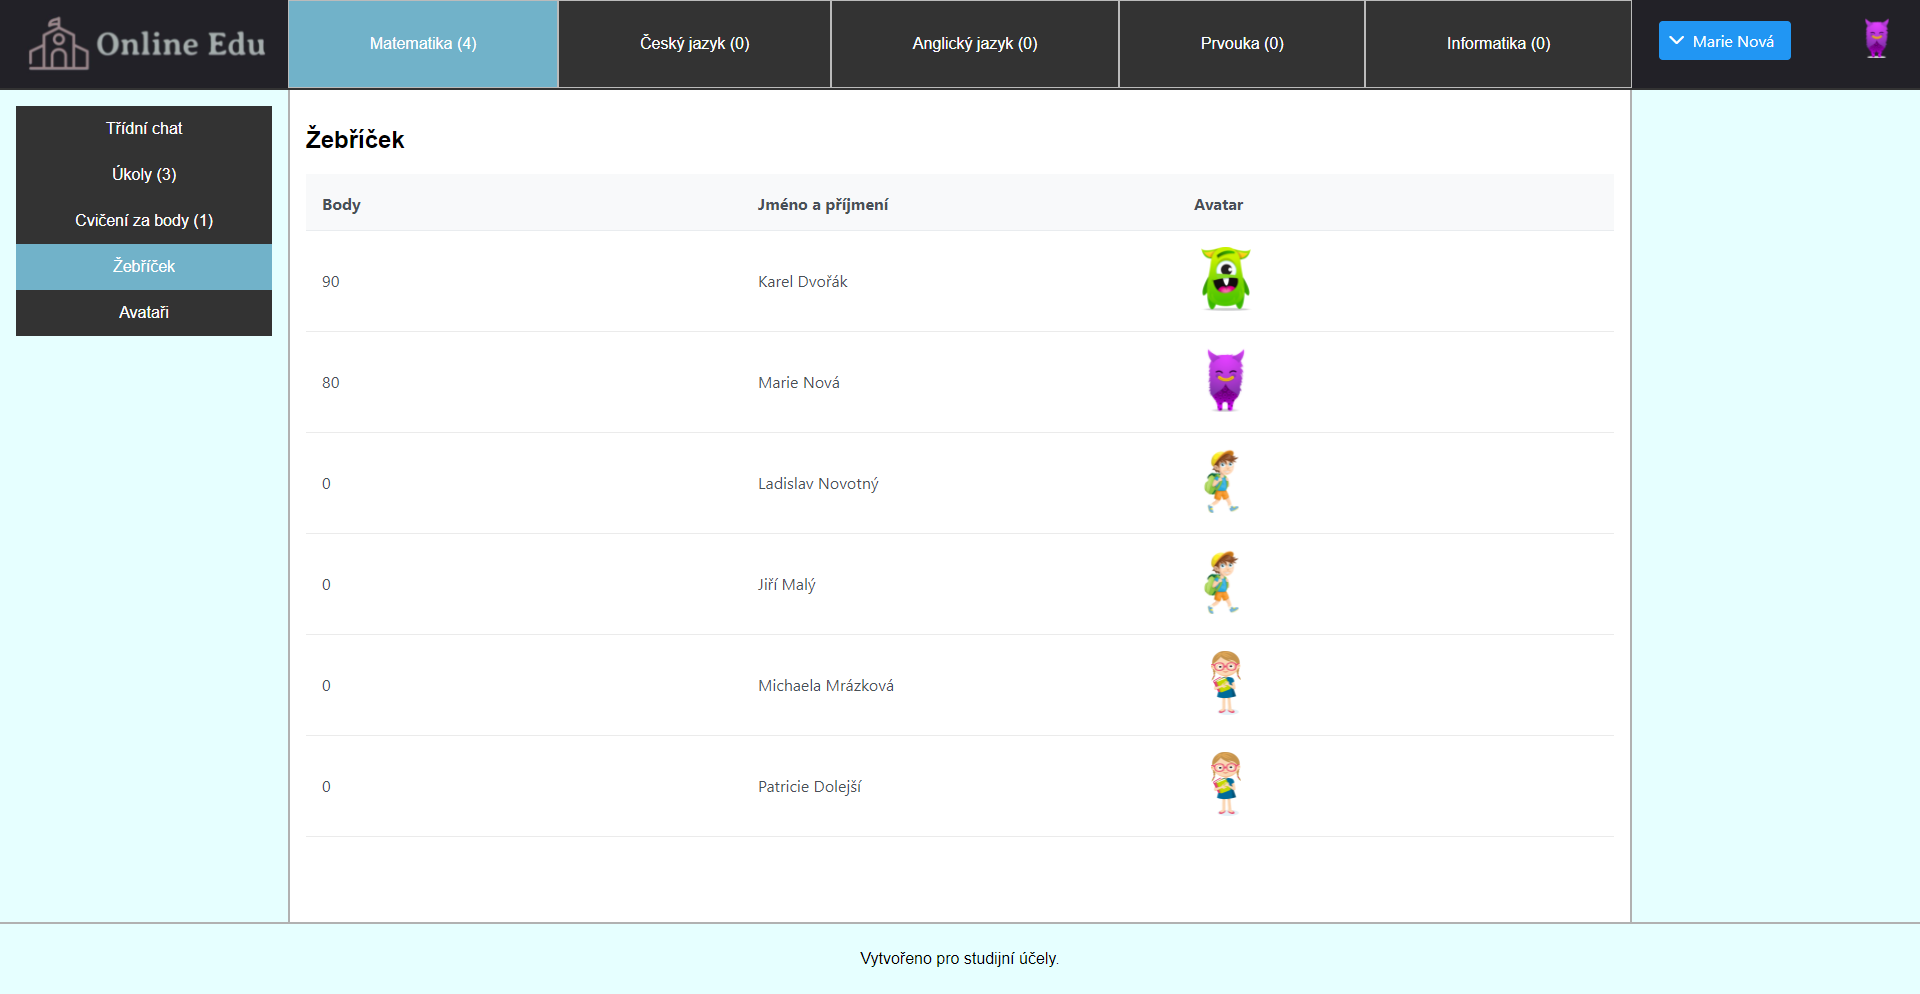
\includegraphics[width=\textwidth]{images/app_screenshots/zak_zebricek}
\end{figure}

Ze svých vlastněných avatarů může student také vybírat přímo na své profilové stránce na obrázku \ref{ref:student-profil}. Mimo to si zde i může měnit své heslo.
\begin{figure}[H]
    \caption{Student -- profil}
    \label{ref:student-profil}
    \centering
    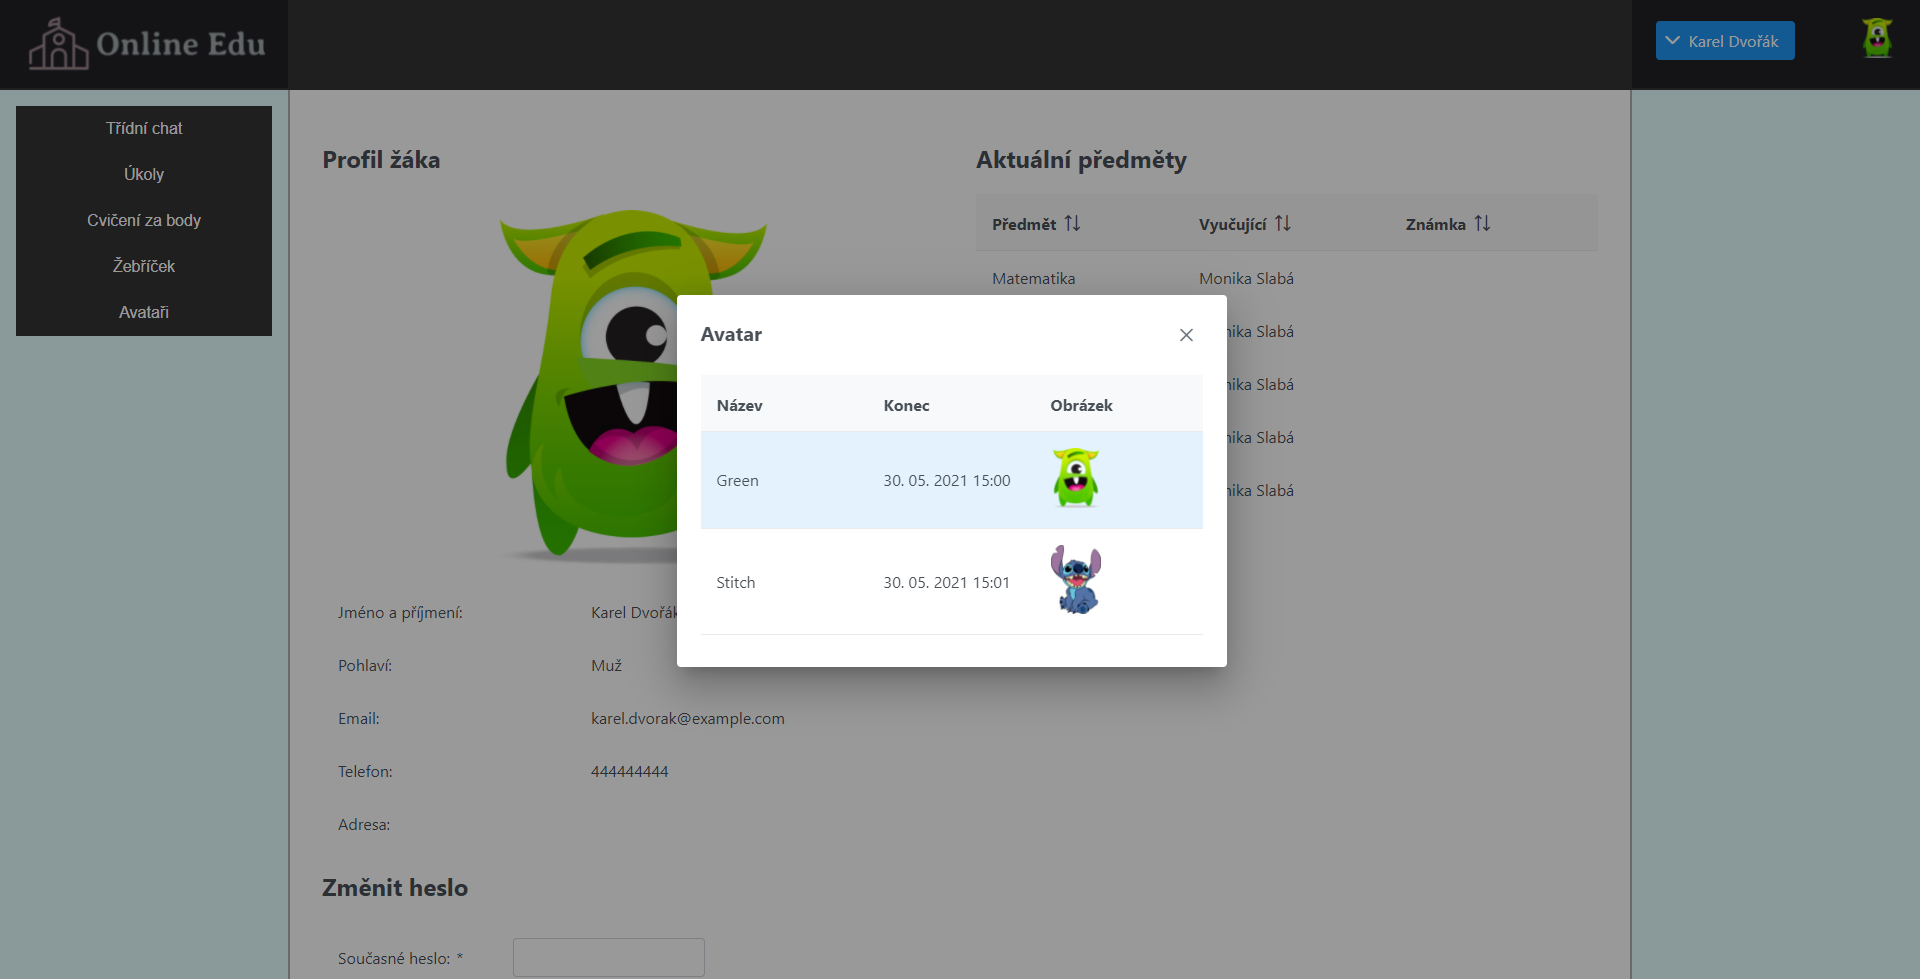
\includegraphics[width=\textwidth]{images/app_screenshots/zak_profil_zmena.png}
\end{figure}

\section{Rozhraní pro administrátory}

Administrátorské rozhraní umožňuje v podstatě vytvářet a upravovat potřebné entity v systému. Například na obrázku \ref{ref:admin-seznam-zaku} je vidět seznam všech žáků, kde každého z nich lze upravit a nebo vytvářet nové.
\begin{figure}[H]
    \caption{Administrátor -- seznam žáků}
    \label{ref:admin-seznam-zaku}
    \centering
    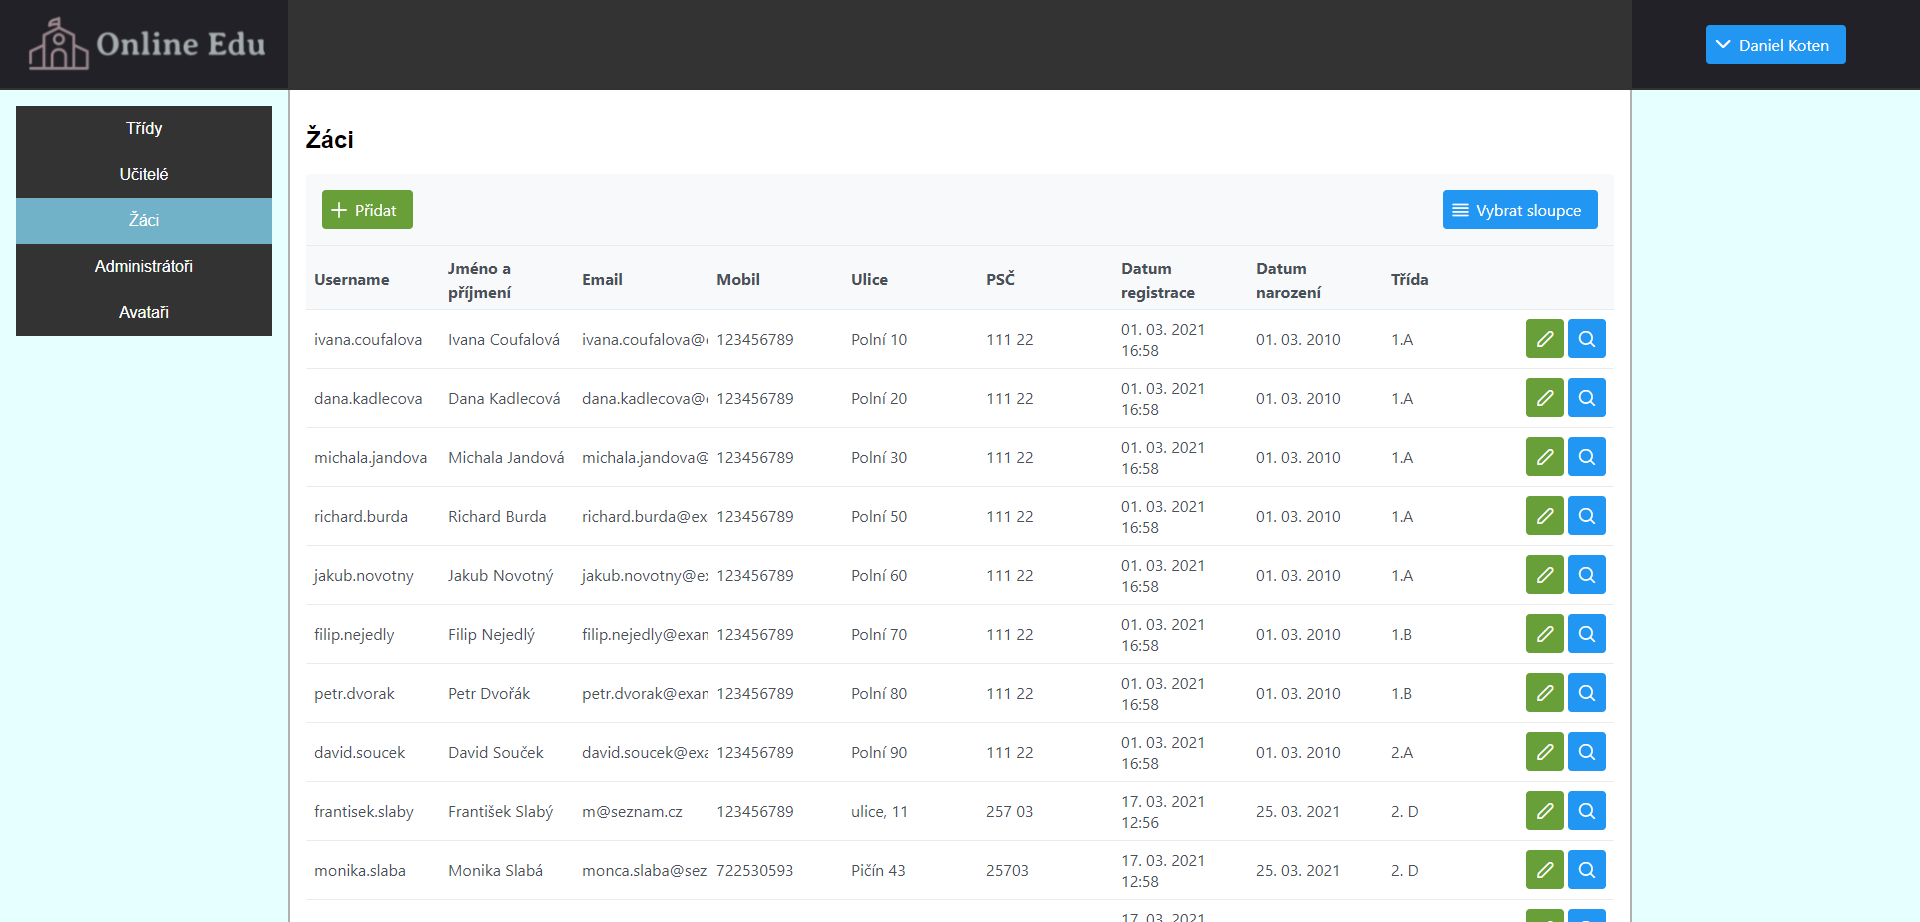
\includegraphics[width=\textwidth]{images/app_screenshots/admin_seznam_zaku}
\end{figure}




\chapter{Průchody aplikací}
\label{chap:prikladne-pruchody}


V této kapitole uvedu několik průchodů aplikací pro nejdůležitější případy užití a také jejich vzájemné porovnání v různých verzích implementace. Jelikož by měl být systém v první řadě co nejjednodušší, tak jsem cítil potřebu tuto jednoduchost také nějak měřit. Samozřejmě, že míra jednoduchosti je z velké části velmi subjektivní a co se někomu může zdát snadné a přehledné, tak pro druhého může být příliš komplexní. Nicméně jako takovou zjednodušenou a vyčíslitelnou míru jednoduchosti jsem použil počet pomyslných kroků pro dosáhnutí určitého cíle. Například počet kliknutí, vyplnění polí, nutnost najít řádek v dlouhé tabulce atd.

První verzí je myšlena verze po dokončení předmětu Semestrální projekt. Tato verze byla sice z velké části kompletní z pohledu funkcionalit, nicméně ještě obsahovala spoustu nedokonalostí, zejména co se týče uživatelského komfortu. Spousta činností byla řešena velmi těžkopádně, zdlouhavě a neintuitivně.

Druhá verze je finální řešení po zaimplementování komentářů a postřehů, které vzešly z konzultací s vedoucím práce, z mé vlastní uživatelské zkušenosti a v neposlední řadě od kamarádů a známých učitelek, které mi pomohly s uživatelským testováním.
V této verzi se ohledně počtů kroků počítá s tím, že má uživatel konkrétní stránku uloženou v záložkách prohlížeče.



\section{Zadání nového úkolu}
Pro zadání úkolu nyní stačí pouze přejít na příslušnou stránku uloženou v záložkách, vyplnit text zadání a přidat jej.

\begin{table}[H]
    \centering
    \rowcolors{2}{tablelightblue}{tableblue}
    \begin{tabular}{ |p{0.5\textwidth}|p{0.5\textwidth}| } 
        \hline
        \rowcolor{tabledarkblue}
        První verze & Druhá verze\\
        \hline
        Kliknout na tlačítko přihlášení & Přejít na stránku seznam úkolů \\ 
        Zadat údaje & Vyplnit zadání a vytvořit nový úkol \\ 
        Přihlásit se & \\ 
        Přejít na hlavní stránku učitele & \\
        Zobrazit seznam úkolů & \\
        Vyplnit zadání a vytvořit nový úkol & \\
        \hline
    \end{tabular}
    \caption{Zadání nového úkolu}
    \label{table:newTask}
\end{table}


\section{Odevzdání úkolu}
Pro přidání řešení již není nutné hledat konkrétní položku v seznamu všech úkolů, ale stačí rovnou přejít na seznam těch nedokončených.

\begin{table}[H]
    \centering
    \rowcolors{2}{tablelightblue}{tableblue}
    \begin{tabular}{ |p{0.5\textwidth}|p{0.5\textwidth}| } 
        \hline
        \rowcolor{tabledarkblue}
        První verze & Druhá verze\\
        \hline
        Kliknout na tlačítko přihlášení & Přejít na stránku seznam nedokončených úkolů \\ 
        Zadat údaje & Zvolit úkol \\ 
        Přihlásit se & Vyplnit a odeslat řešení\\ 
        Přejít na hlavní stránku žáka & \\
        Zobrazit seznam všech úkolů & \\
        Najít v tabulce nový úkol & \\
        Zvolit úkol & \\
        Vyplnit a odeslat řešení & \\
        \hline
    \end{tabular}
    \caption{Odevzdání úkolu}
    \label{table:submitAttempt}
\end{table}


\section{Schválení nebo vrácení pokusu}
Tento bod prošel asi největším vylepšením. Stačí teď pouze přejít na seznam aktuálních úkolů, zobrazit si pouze ty žáky, kteří odeslali nějaké nové řešení a to zkontrolovat. Nebo je možná ještě kratší varianta přejít na novinky, kde se ukazuje posledních 10 odeslaných řešení a zobrazit si ho odtud.

\begin{table}[H]
    \centering
    \rowcolors{2}{tablelightblue}{tableblue}
    \begin{tabular}{ |p{0.5\textwidth}|p{0.5\textwidth}| } 
        \hline
        \rowcolor{tabledarkblue}
        První verze & Druhá verze\\
        \hline
        Kliknout na tlačítko přihlášení & Přejít na seznam úkolů ke kontrole \\ 
        Zadat údaje & Zvolit úkol \\ 
        Přihlásit se & Přejít na žákovo poslední odevzdaný pokus\\ 
        Přejít na hlavní stránku učitele & Napsat zpětnou vazbu\\
        Zobrazit seznam všech úkolů & Schválit nebo vrátit\\
        Najít v tabulce úkol u kterého přibyly pokusy & \\
        Zvolit úkol & \\
        Podívat se na zadání úkolu & \\
        Rozkliknout žákovo pokusy & \\
        Přejít na poslední odevzdaný pokus & \\
        Napsat zpětnou vazbu & \\
        Schválit nebo vrátit & \\
        \hline
    \end{tabular}
    \caption{Schválení nebo vrácení pokusu}
    \label{table:acceptOrReturnAttempt}
\end{table}


\section{Opravné odevzdání úkolu}
Nakonec stojí za zmínku vylepšené opravné odeslání řešení. V první verzi bylo nutné z detailu úkolu přejít přímo na stránku detail pokusu, zde si přečíst zpětnou vazbu, vrátit se a odeslat nové řešení. V nové verzi je vše na jednom místě přímo v detailu úkolu. Zejména minulé pokusy včetně zpětné vazby lze prohlížet v chronologickém pořadí z jednoho místa.

\begin{table}[H]
    \centering
    \rowcolors{2}{tablelightblue}{tableblue}
    \begin{tabular}{ |p{0.5\textwidth}|p{0.5\textwidth}| } 
        \hline
        \rowcolor{tabledarkblue}
        První verze & Druhá verze\\
        \hline
        Kliknout na tlačítko přihlášení & Přejít na stránku seznam nedokončených úkolů \\ 
        Zadat údaje & Zvolit úkol \\ 
        Přihlásit se & Přečíst si poslední komentář ve sloupci s minulými pokusy\\ 
        Přejít na hlavní stránku žáka & Vyplnit nové řešení a odeslat\\
        Zobrazit seznam všech úkolů & \\
        Najít v tabulce vrácený úkol & \\
        Zvolit úkol & \\
        Přejít na pokus, který byl vrácen k přepracování & \\
        Přečíst si komentář & \\
        Vrátit se zpět na zadání úkolu & \\
        Vyplnit nové řešení a odeslat & \\
        \hline
    \end{tabular}
    \caption{Opravné odevzdání úkolu}
    \label{table:resubmitAttempt}
\end{table}



\section{Shrnutí}
Z předchozích srovnání je vidět, že se celý proces velice zjednodušil zejména v oblasti přihlašování. Toho jsem docílil prodloužením času \uv{sezení} a vyladěním správného přesměrovávání po samotném přihlášení. Nicméně do budoucna mě později napadla ještě lepší varianta -- tzv. zůstat přihlášený. Uživatel by zadal přihlašovací údaje pouze poprvé, kde si může zvolit možnost, aby si ho prohlížeč pamatoval. Tím se mu do cookies uloží unikátní přihlašovací token, který se následně používá k automatické autorizaci i autentizaci. Token má samozřejmě svou omezenou platnost, která lze libovolně nastavit a po její expiraci se musí uživatel znovu ručně přihlásit, což je ovšem v porovnání s klasickým přihlašováním zanedbatelné ztížení.

Další pozorovatelné zjednodušení vidím v rozdělení úkolů přímo na nedokončené, odeslané a hotové z pohledu žáka a na nedokončené a hotové z pohledu učitele. Tím nemusí ani jedna strana hledat v dlouhém seznamu všech možných úkolů a jednoduše si vždy otevře jen ty aktuální.

V neposlední řadě lze vidět zlepšení i v propracovanější stránce detail úkolu u žáka, kde může student procházet všechny v minulosti odeslané pokusy včetně jejich náhledu. Pro přečtení komentáře od učitele tedy nemusí žák nutně rozklikávat každý pokus, ale vidí vše na jednom místě.


\chapter{Testování}
Pro účely testování jsem po dohodě se svým vedoucím využil nástroj pro automatické testování webových aplikací Selenium IDE \cite{selenium}. Samotné testy se dají vytvářet tak, že se v podstatě zaznamenají provedené akce na stránce a v budoucnu se již provedou automaticky. Samozřejmě je možné přidávat i kroky pro kontrolu, zda se na stránce nachází nějaký element nebo zda je v určitém poli správná hodnota.

Ve své práci jsem vytvořil 15 různých akceptačních testů, které testují nejdůležitější případy užití. Jednoduchou ukázku lze vidět na obrázku \ref{img:selenium}.

Testy se nejprve zkusí přihlásit jako administrátor a vytvořit několik entit, jako například třídy, učitele a studenty. Nově vytvořeným uživatelům nastaví nové heslo a následně se odhlásí.

Dále se pokusí přihlásit jako učitel a vytvořit několik nových úkolů. Poté, co tyto úkoly jako student vyplní a odešle, tak některé schválí a některé vrátí k přepracování. Po opětovném odevzdání vrácených úkolů i tyto schválí.

Po úspěšném projití všech těchto testů je ověřena většina případů užití.

\begin{figure}
    \caption{Ukázka testů v Selenium IDE}
    \centering
    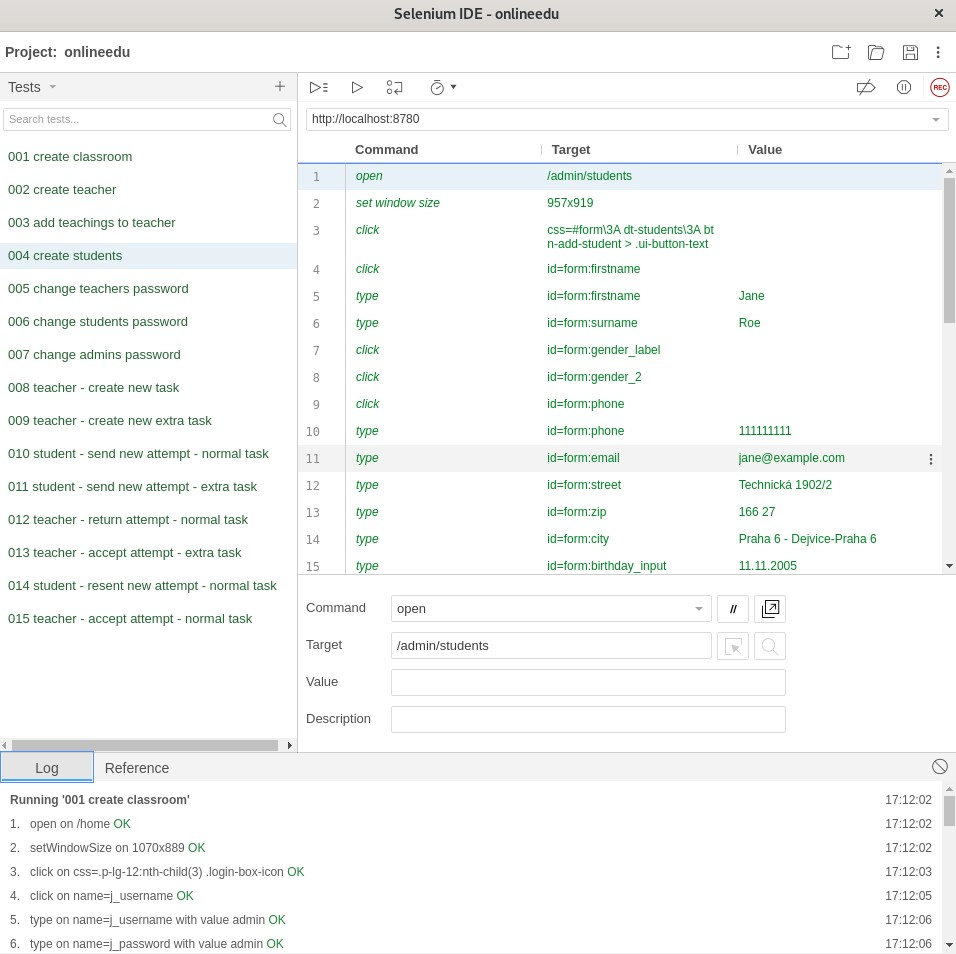
\includegraphics[width=\textwidth]{images/selenium}
    \label{img:selenium}
\end{figure}

\chapter{Závěr}

%Ve své práci jsem se snažil pokrýt zejména nedostatky stávajících systémů. Jako příklad bych mohl uvést několik těchto bodů s krátkým komentářem, jak jsem daný problém řešil.

Ve své práci jsem se soustředil zejména na práci s úkoly a jejich stavy, což je častý problém současných systémů. Nesnažil jsem se o kompletní řešení celé problematiky. Spíše jsem chtěl ukázat možný způsob implementace speciálně pro danou oblast.

Hlavním požadavkem byla jednoduchost. Na obrázku \ref{ref:ucitel-seznam-ukolu} na stránce \pageref{ref:ucitel-seznam-ukolu} je vidět příklad toho, jak jsem si s tímto bodem poradil. Maximální přehlednosti zde přispívá zejména rozvržení uživatelského rozhraní. V~horní části lze jednoduše přepínat mezi třídami a předměty a pro každou tuto kombinaci lze pak v~levém menu volit různé stránky. Uživatel také v každé chvíli přesně ví, kde se nachází díky barevnému zvýraznění v~navigačních menu. 

Kromě samotné navigace nabízí obě menu i notifikace. U každé třídy a předmětu vidí uživatel počty záležitostí, které by měl vyřešit (např. počty úkolů k opravení). Díky tomu by se pak nemělo stávat, že někdo na něco zapomene. Jednoduše se učitel či žák přihlásí a ihned ví, kam kliknout.

Neméně důležité bylo také potřeba rozmyslet, jak bude systém s úkoly, zejména jejich stavy, vlastně pracovat. Výstižně mé řešení popisuje stavový diagram úkolu \ref{fig:taskStateDiagram} na stránce \pageref{fig:taskStateDiagram}, kde lze vidět kompletní životní cyklus úkolu. Ve stručnosti je důležité zejména to, že když se úkol nachází v pro uživatele nezajímavém stavu (pro žáka např. stav odesláno), tak tento úkol nevidí v~hlavním seznamu úkolů, kde by mělo být opravdu jen to, co je potřeba právě teď udělat.

Dalším velkým problémem, který je potřeba řešit, je registrace uživatelů a vytváření tříd. Já jsem se rozhodl pro to, že tyto entity bude vždy vytvářet nadřízená osoba, která je v daném ohledu většinou vzdělanější. Například žákům vytvoří účty učitel a těm je zase včetně tříd a předmětů vytvoří administrátor. Z mého pohledu je takový přístup zejména pro žáky mnohem jednodušší a přímočařejší, než aby si museli vytvářet účet sami a následně se přihlašovat do různých předmětů.

Nad rámec zadání jsem také implementoval různé herní prvky včetně třídního chatu (vizte kapitolu \ref{chap:gamifikace}, \nameref{chap:gamifikace}). Hlavní pointou je získávání bodů za dobrovolné úkoly, za které si žák následně může vybrat svého avatara. Toho pak používá u svých zpráv v třídním chatu a také v třídním žebříčku.

Zadáním mé bakalářské práce bylo implementovat systém pro zjednodušení úkonů ze strany učitelů a žáků na základních školách. Zejména jsem se měl soustředit na práci s domácími úkoly, a to z uživatelského hlediska v maximální jednoduchosti. Tohoto směru jsem se držel a rozhodně je tedy možné pro tuto oblast začít výsledný systém reálně používat. Co se ovšem týče dalších oblastí, určitě zde vidím spoustu dalších možností k pokračovaní například formou diplomové práce. Kromě nápadů jako videohovory, rozvrhy, zapisování absence a dalších tradičních funkcí si konkrétně dovedu představit například pokročilejší a dynamičtější formu již zmíněné gamifikace skrze předpřipravené výukové hry, za které by žáci mohli získávat body. Všechna tato rozšíření není do budoucna problém do mé aplikace doimplementovat. Dokonce nic nebrání tomu přidat REST rozhraní a nový modul vyvíjet naprosto nezávisle v jiné technologii.














\appendix

\printindex

%\appendix

\bibliographystyle{unsrt}
\bibliography{onlineedu}

%\appendix



%\appendix
\chapter{Instalace}

Zdrojové soubory lze stáhnout z GitHub repozitáře na adrese \url{https://github.com/koty10/online-edu}.

Dále bude potřeba JDK 11 (Java Development Kit), který lze stáhnout z \url{https://www.oracle.com/java/technologies/javase-jdk11-downloads.html}.

Pro zprovoznění aplikace vřele doporučuji nainstalovat kontejnerovou technologii Docker \cite{docker} (spolu s Docker Compose). Pak stačí v adresáři /docker/ pouze spustit tyto skripty.
\begin{itemize}
    \item 01-build-src-local-docker.sh
    \item 02-build-dockers.sh
    \item 03-run.sh
\end{itemize}

Aplikace, je poté přístupná na adrese \url{http://localhost:8780/home}.

Pokud jde jen o prohlédnutí běžící aplikace, tak je samozřejmě možné si ji otevřít přímo na \uv{produkčním} prostředí na adrese \url{https://online-edu.aubrecht.net/home}.



\nomenclature{BE}{Backend -- vrstva pracující s daty a logikou aplikace}
\nomenclature{FE}{Frontend -- prezentační vrstva pracující zejména se vzhledem aplikace}
\nomenclature{AJAX}{Asynchronous JavaScript and XML -- časté označení pro asynchronní zpracování webových požadavků bez nutnosti znovunačtení stránky}
\nomenclature{OS}{Operační systém}
\nomenclature{RAM}{Operační paměť}
\nomenclature{ORM}{Objektově relační mapování -- přístup umožňující práci s tabulkami uložené v relační databázi podobně jako s objekty}
\nomenclature{JSF}{JavaServer Faces}
\nomenclature{TCP}{Transmission Control Protocol -- protokol transportní vrstvy TCP/IP}
\nomenclature{API}{Application Programming Interface -- definované rozhraní pro komunikaci s nějakou částí systému}
\nomenclature{JDBC}{Java Database Connectivity -- rozhraní pro práci s databází v jazyku Java}
\nomenclature{JPA}{Java Persistence API -- standard umožňující ORM, existuje několik implementací}
\nomenclature{FP}{Funkční požadavek}
\nomenclature{NP}{Nefunkční požadavek}
\nomenclature{REST}{Representational State Transfer}

\printnomenclature


%\ctutemplate{specification.as.chapter}

\end{document}